% Options for packages loaded elsewhere
% Options for packages loaded elsewhere
\PassOptionsToPackage{unicode}{hyperref}
\PassOptionsToPackage{hyphens}{url}
\PassOptionsToPackage{dvipsnames,svgnames,x11names}{xcolor}
%
\documentclass[
  letterpaper,
  DIV=11,
  numbers=noendperiod]{scrreprt}
\usepackage{xcolor}
\usepackage{amsmath,amssymb}
\setcounter{secnumdepth}{5}
\usepackage{iftex}
\ifPDFTeX
  \usepackage[T1]{fontenc}
  \usepackage[utf8]{inputenc}
  \usepackage{textcomp} % provide euro and other symbols
\else % if luatex or xetex
  \usepackage{unicode-math} % this also loads fontspec
  \defaultfontfeatures{Scale=MatchLowercase}
  \defaultfontfeatures[\rmfamily]{Ligatures=TeX,Scale=1}
\fi
\usepackage{lmodern}
\ifPDFTeX\else
  % xetex/luatex font selection
\fi
% Use upquote if available, for straight quotes in verbatim environments
\IfFileExists{upquote.sty}{\usepackage{upquote}}{}
\IfFileExists{microtype.sty}{% use microtype if available
  \usepackage[]{microtype}
  \UseMicrotypeSet[protrusion]{basicmath} % disable protrusion for tt fonts
}{}
\makeatletter
\@ifundefined{KOMAClassName}{% if non-KOMA class
  \IfFileExists{parskip.sty}{%
    \usepackage{parskip}
  }{% else
    \setlength{\parindent}{0pt}
    \setlength{\parskip}{6pt plus 2pt minus 1pt}}
}{% if KOMA class
  \KOMAoptions{parskip=half}}
\makeatother
% Make \paragraph and \subparagraph free-standing
\makeatletter
\ifx\paragraph\undefined\else
  \let\oldparagraph\paragraph
  \renewcommand{\paragraph}{
    \@ifstar
      \xxxParagraphStar
      \xxxParagraphNoStar
  }
  \newcommand{\xxxParagraphStar}[1]{\oldparagraph*{#1}\mbox{}}
  \newcommand{\xxxParagraphNoStar}[1]{\oldparagraph{#1}\mbox{}}
\fi
\ifx\subparagraph\undefined\else
  \let\oldsubparagraph\subparagraph
  \renewcommand{\subparagraph}{
    \@ifstar
      \xxxSubParagraphStar
      \xxxSubParagraphNoStar
  }
  \newcommand{\xxxSubParagraphStar}[1]{\oldsubparagraph*{#1}\mbox{}}
  \newcommand{\xxxSubParagraphNoStar}[1]{\oldsubparagraph{#1}\mbox{}}
\fi
\makeatother

\usepackage{color}
\usepackage{fancyvrb}
\newcommand{\VerbBar}{|}
\newcommand{\VERB}{\Verb[commandchars=\\\{\}]}
\DefineVerbatimEnvironment{Highlighting}{Verbatim}{commandchars=\\\{\}}
% Add ',fontsize=\small' for more characters per line
\usepackage{framed}
\definecolor{shadecolor}{RGB}{241,243,245}
\newenvironment{Shaded}{\begin{snugshade}}{\end{snugshade}}
\newcommand{\AlertTok}[1]{\textcolor[rgb]{0.68,0.00,0.00}{#1}}
\newcommand{\AnnotationTok}[1]{\textcolor[rgb]{0.37,0.37,0.37}{#1}}
\newcommand{\AttributeTok}[1]{\textcolor[rgb]{0.40,0.45,0.13}{#1}}
\newcommand{\BaseNTok}[1]{\textcolor[rgb]{0.68,0.00,0.00}{#1}}
\newcommand{\BuiltInTok}[1]{\textcolor[rgb]{0.00,0.23,0.31}{#1}}
\newcommand{\CharTok}[1]{\textcolor[rgb]{0.13,0.47,0.30}{#1}}
\newcommand{\CommentTok}[1]{\textcolor[rgb]{0.37,0.37,0.37}{#1}}
\newcommand{\CommentVarTok}[1]{\textcolor[rgb]{0.37,0.37,0.37}{\textit{#1}}}
\newcommand{\ConstantTok}[1]{\textcolor[rgb]{0.56,0.35,0.01}{#1}}
\newcommand{\ControlFlowTok}[1]{\textcolor[rgb]{0.00,0.23,0.31}{\textbf{#1}}}
\newcommand{\DataTypeTok}[1]{\textcolor[rgb]{0.68,0.00,0.00}{#1}}
\newcommand{\DecValTok}[1]{\textcolor[rgb]{0.68,0.00,0.00}{#1}}
\newcommand{\DocumentationTok}[1]{\textcolor[rgb]{0.37,0.37,0.37}{\textit{#1}}}
\newcommand{\ErrorTok}[1]{\textcolor[rgb]{0.68,0.00,0.00}{#1}}
\newcommand{\ExtensionTok}[1]{\textcolor[rgb]{0.00,0.23,0.31}{#1}}
\newcommand{\FloatTok}[1]{\textcolor[rgb]{0.68,0.00,0.00}{#1}}
\newcommand{\FunctionTok}[1]{\textcolor[rgb]{0.28,0.35,0.67}{#1}}
\newcommand{\ImportTok}[1]{\textcolor[rgb]{0.00,0.46,0.62}{#1}}
\newcommand{\InformationTok}[1]{\textcolor[rgb]{0.37,0.37,0.37}{#1}}
\newcommand{\KeywordTok}[1]{\textcolor[rgb]{0.00,0.23,0.31}{\textbf{#1}}}
\newcommand{\NormalTok}[1]{\textcolor[rgb]{0.00,0.23,0.31}{#1}}
\newcommand{\OperatorTok}[1]{\textcolor[rgb]{0.37,0.37,0.37}{#1}}
\newcommand{\OtherTok}[1]{\textcolor[rgb]{0.00,0.23,0.31}{#1}}
\newcommand{\PreprocessorTok}[1]{\textcolor[rgb]{0.68,0.00,0.00}{#1}}
\newcommand{\RegionMarkerTok}[1]{\textcolor[rgb]{0.00,0.23,0.31}{#1}}
\newcommand{\SpecialCharTok}[1]{\textcolor[rgb]{0.37,0.37,0.37}{#1}}
\newcommand{\SpecialStringTok}[1]{\textcolor[rgb]{0.13,0.47,0.30}{#1}}
\newcommand{\StringTok}[1]{\textcolor[rgb]{0.13,0.47,0.30}{#1}}
\newcommand{\VariableTok}[1]{\textcolor[rgb]{0.07,0.07,0.07}{#1}}
\newcommand{\VerbatimStringTok}[1]{\textcolor[rgb]{0.13,0.47,0.30}{#1}}
\newcommand{\WarningTok}[1]{\textcolor[rgb]{0.37,0.37,0.37}{\textit{#1}}}

\usepackage{longtable,booktabs,array}
\usepackage{calc} % for calculating minipage widths
% Correct order of tables after \paragraph or \subparagraph
\usepackage{etoolbox}
\makeatletter
\patchcmd\longtable{\par}{\if@noskipsec\mbox{}\fi\par}{}{}
\makeatother
% Allow footnotes in longtable head/foot
\IfFileExists{footnotehyper.sty}{\usepackage{footnotehyper}}{\usepackage{footnote}}
\makesavenoteenv{longtable}
\usepackage{graphicx}
\makeatletter
\newsavebox\pandoc@box
\newcommand*\pandocbounded[1]{% scales image to fit in text height/width
  \sbox\pandoc@box{#1}%
  \Gscale@div\@tempa{\textheight}{\dimexpr\ht\pandoc@box+\dp\pandoc@box\relax}%
  \Gscale@div\@tempb{\linewidth}{\wd\pandoc@box}%
  \ifdim\@tempb\p@<\@tempa\p@\let\@tempa\@tempb\fi% select the smaller of both
  \ifdim\@tempa\p@<\p@\scalebox{\@tempa}{\usebox\pandoc@box}%
  \else\usebox{\pandoc@box}%
  \fi%
}
% Set default figure placement to htbp
\def\fps@figure{htbp}
\makeatother





\setlength{\emergencystretch}{3em} % prevent overfull lines

\providecommand{\tightlist}{%
  \setlength{\itemsep}{0pt}\setlength{\parskip}{0pt}}



 


\usepackage{booktabs}
\usepackage{longtable}
\usepackage{array}
\usepackage{multirow}
\usepackage{wrapfig}
\usepackage{float}
\usepackage{colortbl}
\usepackage{pdflscape}
\usepackage{tabu}
\usepackage{threeparttable}
\usepackage{threeparttablex}
\usepackage[normalem]{ulem}
\usepackage{makecell}
\usepackage{xcolor}
\KOMAoption{captions}{tableheading}
\makeatletter
\@ifpackageloaded{bookmark}{}{\usepackage{bookmark}}
\makeatother
\makeatletter
\@ifpackageloaded{caption}{}{\usepackage{caption}}
\AtBeginDocument{%
\ifdefined\contentsname
  \renewcommand*\contentsname{Table of contents}
\else
  \newcommand\contentsname{Table of contents}
\fi
\ifdefined\listfigurename
  \renewcommand*\listfigurename{List of Figures}
\else
  \newcommand\listfigurename{List of Figures}
\fi
\ifdefined\listtablename
  \renewcommand*\listtablename{List of Tables}
\else
  \newcommand\listtablename{List of Tables}
\fi
\ifdefined\figurename
  \renewcommand*\figurename{Figure}
\else
  \newcommand\figurename{Figure}
\fi
\ifdefined\tablename
  \renewcommand*\tablename{Table}
\else
  \newcommand\tablename{Table}
\fi
}
\@ifpackageloaded{float}{}{\usepackage{float}}
\floatstyle{ruled}
\@ifundefined{c@chapter}{\newfloat{codelisting}{h}{lop}}{\newfloat{codelisting}{h}{lop}[chapter]}
\floatname{codelisting}{Listing}
\newcommand*\listoflistings{\listof{codelisting}{List of Listings}}
\makeatother
\makeatletter
\makeatother
\makeatletter
\@ifpackageloaded{caption}{}{\usepackage{caption}}
\@ifpackageloaded{subcaption}{}{\usepackage{subcaption}}
\makeatother
\usepackage{bookmark}
\IfFileExists{xurl.sty}{\usepackage{xurl}}{} % add URL line breaks if available
\urlstyle{same}
\hypersetup{
  pdftitle={Practical Ecology book},
  pdfauthor={Tamsyn Kiss},
  colorlinks=true,
  linkcolor={blue},
  filecolor={Maroon},
  citecolor={Blue},
  urlcolor={Blue},
  pdfcreator={LaTeX via pandoc}}


\title{Practical Ecology book}
\author{Tamsyn Kiss}
\date{24 April, 2026}
\begin{document}
\maketitle

\renewcommand*\contentsname{Table of contents}
{
\hypersetup{linkcolor=}
\setcounter{tocdepth}{2}
\tableofcontents
}

\bookmarksetup{startatroot}

\chapter*{Preface}\label{preface}
\addcontentsline{toc}{chapter}{Preface}

\markboth{Preface}{Preface}

This is a Quarto book.

To learn more about Quarto books visit
\url{https://quarto.org/docs/books}.

\begin{Shaded}
\begin{Highlighting}[]
\DecValTok{1} \SpecialCharTok{+} \DecValTok{1}
\end{Highlighting}
\end{Shaded}

\begin{verbatim}
[1] 2
\end{verbatim}

\bookmarksetup{startatroot}

\chapter*{Introduction}\label{introduction}
\addcontentsline{toc}{chapter}{Introduction}

\markboth{Introduction}{Introduction}

Welcome to the Practical Ecology textbook!

In this textbook, you will find the content chapters for the Practical
Ecology module, along with workshop activities and the dedicated R code
necessary to understand and reproduce the analysis in R.

\section*{Module aims:}\label{module-aims}
\addcontentsline{toc}{section}{Module aims:}

\markright{Module aims:}

Students who successfully complete this module will be able to:

\begin{enumerate}
\def\labelenumi{\arabic{enumi}.}
\tightlist
\item
  Choose, use and critique sampling techniques for plant and animal
  populations.
\item
  Choose, use and critique analysis methods for ecological sampling
  data.
\item
  Interpret and discuss patterns of ecological populations and
  communities, with reference to theory and the environments in which
  they are found.
\item
  Design and evaluate experiments to sample plant and animal
  populations, and explain how these address ecological hypotheses.
\item
  Work in a small group to develop and carry out a field research
  project.
\item
  Communicate and discuss ecological fieldwork methods, results and
  implications to a scientific audience.
\end{enumerate}

\section*{How to study this module}\label{how-to-study-this-module}
\addcontentsline{toc}{section}{How to study this module}

\markright{How to study this module}

\textbf{Taught topics} are covered through a series of online resources,
practicals and workshops addressing practical and theoretical aspects of
plant and animal sampling, and data analysis and interpretation for
populations and communities, all within a central theme of experimental
design. Each week, learning materials will be available on the VLE to
introduce and contextualise the topics under consideration. Active
learning by students individually and in groups will build upon
structured private study and formative assessment using virtual
communities, analysis in R, practical work and an online repository of
class outputs. Emphasis is placed on critically interpreting and
communicating the data and information gained by these techniques and
understanding their limitations, and reflecting on students' own
development as researchers and practitioners in ecology.

\textbf{During the field course}, the students will have the opportunity
to discover more directly how organisms live in their environment, and
to develop and execute an ecological investigation in small groups for 5
days. After introduction to a range of habitats, the students, under the
supervision of a member of staff, will be responsible for (1) defining
the aim of their study, (2) coming up with a sensible scientific design
in one of the available sites, (3) carrying out the survey or
experiment, and (4) processing the samples and analysing and
communicating the results.

The first part of the semester will walk you through ideas relating to
the following three questions:

\begin{itemize}
\tightlist
\item
  How can we collect data about the presence and abundance of plants and
  animals?
\item
  Why are organisms present in specific environments?
\item
  What is it about species, populations and environments that shapes
  communities?
\end{itemize}

We'll cover things that don't move (e.g.~most plants), things that do
move (e.g.~most animals), commonness and rarity, species richness,
ecological diversity indices, community similarity, and relating
communities to their environments.

\part{Chapter 1: Organisms that do not move}

The theme for this week's Practical Ecology is the sampling of immobile
organisms: organisms that do not move. This can be done in a variety of
ways, but the most common is to assess the number of individuals in a
set area. That area might be quite large for trees, such as a hectare
(100 x 100 metres), but for smaller organisms it is normal to use a
metre square or even smaller. For example, if you carry out fieldwork on
the rocky shores of Cumbrae at the end of the module, you might use a 10
cm by 10 cm area to count snails or barnacles. Once you have assessed
(by counting, estimating or using an index) the number of individuals
appearing in a set area, you can start to infer things about the ecology
of the population.

In this chapter, we will start with an exploration of how individuals
might be arranged in space (Chapter~\ref{sec-poisson}), think about
qualitative and quantitative ways of counting individuals
(Chapter~\ref{sec-qual-and-quant}), and consider what is an individual
(Chapter~\ref{sec-individual}). There is a practical in which you will
count individual \emph{Plantago lanceolata} on campus. In the workshop
you will assess the spatial distribution of the class \emph{P.
lanceolata} data, and use LEGO® to explore how sampling strategies
affect the effort and biases of population density estimates.

\begin{figure}

\centering{

\pandocbounded{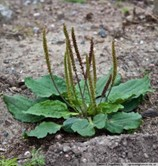
\includegraphics[keepaspectratio]{organisms-that-dont-move/data-image/plantago-1.jpg}}

}

\caption{\label{fig-plantago}An individual Plantago plant growing on a
patch of muddy ground.}

\end{figure}%

\chapter{The Poisson Distribution}\label{sec-poisson}

The Poisson distribution, which is named after a nineteenth century
French mathematician, is the starting point for many ecological
questions.~

\begin{itemize}
\item
  When you count the number of individuals in a set area, for example,
  in a square metre, you might find none, one, two individuals etc.
  These are your observations.
\item
  The Poisson distribution will give you the expected proportion of the
  observations that will have none, one, two, etc (number of individuals
  in the set area) when all the individuals are distributed randomly
  across the wider landscape. These are your expected values.
\item
  We can compare a set of observations with the expected values from the
  Poisson distribution to see if our observed distribution deviates from
  a random (Poisson) one.~
\end{itemize}

\section{Patterns of dispersion}\label{patterns-of-dispersion}

There are two ways that distributions might deviate from the random
distribution shown in Figure~\ref{fig-dispersal} (centre). They might
occur together in clumps (Figure~\ref{fig-dispersal}, right). Here, the
distance between one individual and its closest neighbour(s) is less
than expected in a random distribution.

The alternative is that individuals might be more spread out than
random, or even uniformly distributed across space
(Figure~\ref{fig-dispersal}, left). Here, the distance between one
individual and a close neighbour is more than expected compared to a
random distribution.

\begin{figure}

\centering{

\pandocbounded{\includegraphics[keepaspectratio]{organisms-that-dont-move/data-image/dispersal.png}}

}

\caption{\label{fig-dispersal}Three examples of spatial patterns of
individuals: from left to right, these are overdispersed or regular,
random, and aggregated or clustered.}

\end{figure}%

Let's briefly think about the reasons why you might get these deviations
from random.

\subsection{Clusters}\label{clusters}

If there is very limited dispersal of offspring from the parents,
e.g.~seeds fall right next to the parent, then clumps will naturally
form.

Clusters could also arise from environmental heterogeneity, such as damp
and dry areas. If the species of interest is suited to one environment,
clumps may form in their preferred conditions.

\subsection{Regular patterns}\label{regular-patterns}

If individuals suppress the presence of others, then they will tend to
form a more uniform distribution in space. We call this `overdispersed'
because the individuals are more spread out than you would expect if
they were distributed at random.

\subsection{Overdispersion}\label{overdispersion}

Overdispersed patterns of immobile organisms reflect competition among
individuals for resources.

In the desert, there is a very limited water supply. Individual creosote
bushes (\emph{Larrea tridentata}; Figure~\ref{fig-creosote}) will
deplete the water around themselves once they are established. That
means that no individual can start to grow if it's too near to another
individual because it won't get enough water. The result is that the
bushes are overdispersed; we do not see two individuals close together
as often as we would if the pattern was random or clustered.

\begin{figure}

\centering{

\pandocbounded{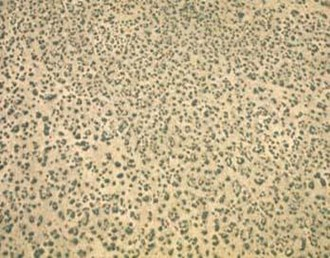
\includegraphics[keepaspectratio]{organisms-that-dont-move/data-image/creosote.jpg}}

}

\caption{\label{fig-creosote}An overhead view of creosote bushes
(\emph{Larrea tridentata}) in a semi-desert area.}

\end{figure}%

This is a pattern that's much more commonly seen in animals, as they
will hold and defend territories. In this case it is the population unit
(such as a family group) that does not move, while individual animals
move across the landscape, within and around the territory.

\subsection{Aggregated}\label{aggregated}

The yellow-wort, \emph{Blackstonia perfoliate},
(Figure~\ref{fig-yellow-wort}) grows best in calcareous soil (high pH,
occurring chiefly on chalk and limestone), so although it is very
widespread in the southern half of the British Isles, it is restricted
to those areas where the soil is suitable
(Figure~\ref{fig-yellow-wort-distribution}). This means that on a very
big scale such as the UK the distribution is very clumped, or
aggregated. Other calcicoles follow a similar pattern.

\begin{figure}

\centering{

\pandocbounded{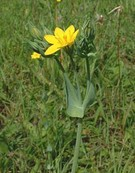
\includegraphics[keepaspectratio]{organisms-that-dont-move/data-image/yellow-wort.jpg}}

}

\caption{\label{fig-yellow-wort}\emph{Blackstonia perfoliata} plant in
flower}

\end{figure}%

\begin{figure}

\begin{minipage}{0.50\linewidth}

\pandocbounded{
\includegraphics[keepaspectratio]{organisms-that-dont-move/data-image/yellow-wort-across-uk.jpg}}

\subcaption{\label{}Yellow-wort distribution}
\end{minipage}%
%
\begin{minipage}{0.50\linewidth}

\pandocbounded{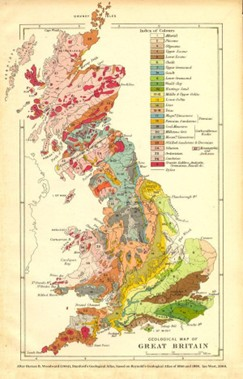
\includegraphics[keepaspectratio]{organisms-that-dont-move/data-image/UK-geological-map.jpg}}

\subcaption{\label{}UK Geological map}
\end{minipage}%

\caption{\label{fig-yellow-wort-distribution}\emph{Blackstonia
perfoliata} distribution across the UK (left) and geological map (right)
showing chalk (6; pale green) and limestone (17, 21-22; turquoise
shades)}

\end{figure}%

Figure~\ref{fig-yellow-wort-distribution} shows the distribution of the
chalk and limestone geology across the UK that is required for the
higher pH soils that the yellow-wort prefers. If you compare the
geological distribution with that of B. perfoliata you will see there's
a very strong overlap, with the plant distribution fitting within the
geology. However, you can also see that the plant's distribution is much
more southern than the geology. This might indicate that there are other
restrictions on where it grows, such as the number or severity of frost
days. If you consider the European range of the species, you would see
that it's mainly a Mediterranean species, so perhaps a northern limit
set by cold is quite likely.

There are other ways that aggregated distributions might occur. One is
by clonal dispersal where plants might reproduce through vegetative
propagation of genetically identical, but independent individuals. These
`parents' are usually called `genets' and the `offspring' are called
`ramets'. We'll come back to an example later in the chapter.

Animals may form groups for a range of reasons. One is the `selfish
herd' where individuals are safer from predators within groups than they
are out on their own because it reduces the `apparency' of each
individual to predators. Another is aggregation of resources, such as
animals near a water source, or in a patch of woodland.

\subsection{Random Distribution}\label{random-distribution}

Populations will be randomly dispersed if there is an equal probability
of an individual successfully occupying any space within the habitat.
This requires species with high dispersal ability and low competition
(inter- or intra-), and a homogenous habitat.

A truly random distribution is actually quite rare in nature. It is only
going to occur in a plant if individuals are equally likely to get
anywhere, so it requires a species with a very high dispersal ability.
Once the seed arrives it can't be picky about the soil, and it can't be
affected by competition, either intra-specific or inter-species. There
are a few species that fit that description but the dandelion,
\emph{Taraxacum officinale}, is one that comes close.

\section{Analysing patterns of
distribution}\label{analysing-patterns-of-distribution}

This week, you will have an opportunity to sample ribwort plantain
(Figure~\ref{fig-individual-ribwort-plantain}) on campus, in a
practical. In the workshop, you will use the data you have collected as
a class to assess whether they are randomly distributed or not, using
the Poisson distribution.

\begin{figure}

\centering{

\pandocbounded{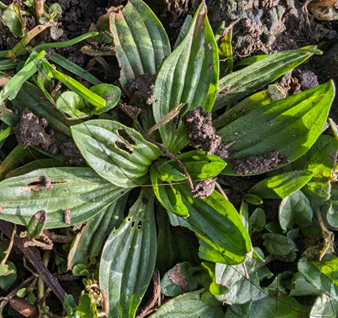
\includegraphics[keepaspectratio]{organisms-that-dont-move/data-image/individual-ribwort-plantain.png}}

}

\caption{\label{fig-individual-ribwort-plantain}An individual ribwort
plantain}

\end{figure}%

As an example, let's use snake's head fritillary, \emph{Fritillaria
meleagris}, and assume we want to analyze the distribution of this
species in a hay meadow. We can imagine that the hay meadow is depicted
as a grid (Figure~\ref{fig-snakes-head-example}).

\begin{figure}

\begin{minipage}{0.50\linewidth}
\pandocbounded{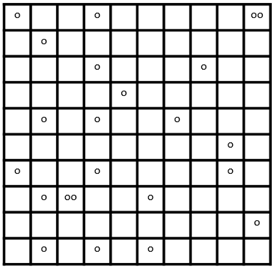
\includegraphics[keepaspectratio]{organisms-that-dont-move/data-image/hay-meadow-grid.png}}\end{minipage}%
%
\begin{minipage}{0.50\linewidth}
\pandocbounded{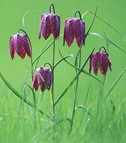
\includegraphics[keepaspectratio]{organisms-that-dont-move/data-image/snakes-head-fritillary.jpg}}\end{minipage}%

\caption{\label{fig-snakes-head-example}Snake's head fritillary
(illustrated on the right): Individual plants (dots) are distributed
across a hay meadow that has been divided into a grid (left).}

\end{figure}%

By dividing the area into the grid of quadrats (square areas of a set
size), and counting the number of organisms per quadrat, we can assess
the mean and variance of the number of plants per quadrat. In this
example, there are 100 quadrats, and 23 individual plants.

The mean number of plants per quadrat is therefore:

\[
\mu =  ({23 \over 100}) = 0.23 
\] Variance indicates the spread of our data, or how variable it is. The
equation for variance is:

\[
\displaystyle \sum_{i = 1}^{N} {(\chi_i - \mu)^2 \over N}
\] In technical terms, this is the average of the squared differences
from the mean. In the equation N is the number of samples (quadrats),
the Greek letter mu (\(\mu\)) is the mean number of individuals per
quadrat, and (\(\chi_i\)) is the individual value. The big Greek sigma
(\(\sum\)) indicates that we're adding up all the values.

One of the really useful characteristics of the Poisson distribution is
that the mean and the variance are the same. We can use this
characteristic as a quantitative basis for deciding on what type of
distribution we are observing.

\section{The Poisson Distribution}\label{the-poisson-distribution}

Before we can do our calculations for the snake's head fritillary, we
need to introduce the Poisson distribution a bit more formally.

It is a discrete distribution describing the number of times an event
occurs in a unit of time or space. This means that you can only get
whole numbers of sightings, and whole units of time or space. This is
useful for count data. When you place a quadrat and count something
(e.g.~the number of individual plants in an area) you're going to get a
whole number and you're going to have a whole number of observations.
For example, you could have recorded 16 quadrats and found 2
individuals, but you can't record 15.8 quadrats with 1.18 individuals.

There are some assumptions that apply if we really have a
\textbf{random} distribution: 1. The mean number of occurrences is small
relative to the maximum possible (i.e.~it's \textbf{rare}). 2.
Occurrences must be \textbf{independent}. 3. Occurrences are
\textbf{random}.

For a Poisson distribution to apply, the number of individuals you can
get into a quadrat must not be limiting. That means you can't use a
quadrat that's so small that it can only possibly have one or two
individuals in it at the most. The other assumptions are that `events'
or `occurrences' (i.e.~each time you see a plant) have to be independent
of each other and random.

In our snake's head fritillary survey of 100 quadrats, we have lots of
quadrats with no plants, some with one, and some with two. In your
survey of \emph{P. lanceolata}, you may have quadrats with up to ten or
fifteen individuals in them. Some years we have found as many as 31
individuals together.

We want to ask the question, what's the probability distribution of the
number of individuals per quadrat? Any problem like this can be fitted
to the discrete Poisson distribution. The Poisson distribution tells us
that the \textbf{expected} number of ``hits'' per trial, if the ``hits''
are randomly distributed, is the mean. In our case, \(\mu\) = 0.23 is
the expected number of plants per quadrat. That is, for every four
quadrats you inspect, you will usually find one plant in one of those
four quadrats.

The Poisson distribution has the property that its \textbf{mean equals
its variance}. Given the mean number of ``hits'' we can generate the
\textbf{probability density function (PDF)} of the distribution. For our
case, the mean number of plants per quadrat is \(\mu\) = 0.23 (23 plants
in 100 quadrats). We therefore already have a prediction: the variance
of number of plants per quadrat should also be 0.23, if the plants are
distributed at random.

\section{The Equation}\label{the-equation}

You will rarely use this equation directly because you can easily get R
to calculate the values, but it is useful to understand how it works,
and to be able to do the calculations `on the back of an envelope' in
those situations where you don't have a computer to hand.

The equation describes the probability \(P(y)\) of a rare event y
occurring in a unit of time or space. This is a function of a single
parameter, \(\mu\), the mean number of occurrences of the event in the
unit time or space.

\[
P(y) = {e^{-\mu} \mu{^y} \over y!}
\]

Here, e (sometimes written exp) is the base of the natural logarithm,
which is 2.718.

The exclamation mark indicates a factorial. That means you have to
multiply all the numbers up to the value. Factorial five would be
written 5! and is calculated as 5x4x3x2x1 = 120.

The factorial of 1 is 1, i.e.~1! = 1. It is convention that 0! is also
1, which is convenient as it prevents `divide by zero' problems in this
equation.

If we look at this equation for zero occurrences (that is when \(y\) =
0, a quadrat has no individuals in it), we would have

\[
P(y = 0) = {e^{-\mu} \mu{^0} \over 0!} = {e^{-\mu} 1 \over 1} = e^{-\mu}
\]

In our example of snake's head fritillary, we had \(\mu\) = 0.23. This
means we can calculate \(P(y = 0) = e^{-\mu} = 2.718 ^{-0.23}\) , to get
the portion of quadrats where we would expect there to be zero
individuals. In this case \(P(y = 0) = 0.7945\), which means that we
would expect around 79\% of the quadrats to have no plants observed in
them if the plants are distributed at random.

\section{Poisson distributions and
biology}\label{poisson-distributions-and-biology}

When you compare the mean and the variance of a distribution, there are
three outcomes:

\begin{enumerate}
\def\labelenumi{\arabic{enumi}.}
\item
  If rare events are random and independent they follow a Poisson
  distribution, and the mean and variance are equal.\\
  \strut \\
  If the mean and variance are similar, we would have no evidence to
  indicate that the distribution isn't random.\\
\item
  If events enhance the chance of other events, the distribution will be
  aggregated, and the variance will be greater than the mean.\\
  \strut \\
  If the variance is greater than the mean we have a situation where
  there are more zero values than we would expect and more big values
  (far above the mean) where there are many individuals together in a
  single quadrat. This increases the variance. This occurs where
  individuals are in clumps or aggregated.
\item
  If events reduce the chance of other events, the distribution will be
  uniform, or overdispersed, and the variance will be less than the
  mean.\\
  \strut \\
  If the variance is less than the mean, we are seeing fewer
  observations higher and lower than the mean and more that are close to
  or at the mean. This reduces the variance and we interpret this as an
  over-dispersed population: the individuals are more spread out than we
  would expect by chance (we find no/few clusters), but also do not fall
  in such a way that any are particularly far from any other individuals
  (we find no/few isolated individuals).
\end{enumerate}

\section{Poisson as a null
hypothesis}\label{poisson-as-a-null-hypothesis}

If the variable is random, the probability distribution will follow a
Poisson distribution. A \(\chi^2\) (chi-squared) goodness-of-fit test
can be carried out to compare observed and expected data and use
statistics to decide whether there is evidence to suggest the observed
distribution differs from the expected one.

If the plants are distributed randomly, the probability of getting 0 or
1 or 2 or 3 etc plants in a quadrat will not be significantly different
from the numbers expected by applying the Poisson probability. That
means we can estimate the values by using the population mean and number
of samples, and use a chi-square goodness of fit test to compare
observations with the Poisson expected values
(Table~\ref{tbl-snakes-head}) To do this by hand, you will need a
chi-square table, which you can look up using R, Sheets or Excel. This
week's R script gives you the code to do these calculations by hand, and
using the \texttt{chisq.test} function.

\begin{longtable}[t]{lllll}

\caption{\label{tbl-snakes-head}Calculations to test whether the snake's
head fritillary is distributed randomly in space. O = Observed, E =
Expected. Here, df = 4, chi squared = 6, and P = 0.1991; there is no
evidence to suggest that the plants are not distributed randomly.}

\tabularnewline

\\
\toprule
 & Number of Plants & Observed Frequency & Expected Frequency & (O-E)\textasciicircum{}2/E\\
\midrule
 & 0 & 79 & 79.45 & 0.0026\\
 & 1 & 19 & 18.27 & 0.0288\\
 & 2 or more & 2 & 2.27 & 0.0326\\
 & Sum & 100 & 100 & 0.064\\
\bottomrule

\end{longtable}

You will have an opportunity to practice the calculations for your
\emph{Plantago} practical data in the workshop (@sec-workshop).

\section{The R code version}\label{the-r-code-version}

First we need to create a vector of the observed counts of Snake's Head
Fritillary. In our field (Figure~\ref{fig-snakes-head-example}) we had
79 quadrats with no plants, 19 quadrats with one plant, and 2 quadrats
with more than one plant, giving us a mean (\(\mu\)) of 0.23

\begin{Shaded}
\begin{Highlighting}[]
\NormalTok{observed }\OtherTok{\textless{}{-}} \FunctionTok{c}\NormalTok{(}\DecValTok{79}\NormalTok{, }\DecValTok{19}\NormalTok{,}\DecValTok{2}\NormalTok{)}
\NormalTok{mu }\OtherTok{\textless{}{-}} \FloatTok{0.23}
\end{Highlighting}
\end{Shaded}

We can also determine the relative probabilites of any quadrat
containing zero, one, or two plants, using the poisson distribution.

The probability of a quadrat containing zero plants is the exponential
of \(\mu\): \(e^{-\mu}\)

\begin{Shaded}
\begin{Highlighting}[]
\NormalTok{Prob\_zero }\OtherTok{\textless{}{-}} \FunctionTok{exp}\NormalTok{(}\SpecialCharTok{{-}}\NormalTok{mu)}
\end{Highlighting}
\end{Shaded}

The probability of a quadrat containing exactly one plant is determined
using the poisson distribution

\begin{Shaded}
\begin{Highlighting}[]
\NormalTok{Prob\_one }\OtherTok{\textless{}{-}} \FunctionTok{dpois}\NormalTok{(}\DecValTok{1}\NormalTok{, mu)}
\end{Highlighting}
\end{Shaded}

And the probability of a quadrat containing two or more plants is 1,
minus the probability of finding one plant, minus the probability of
finding zero plants.

\begin{Shaded}
\begin{Highlighting}[]
\NormalTok{Prob\_two\_or\_more }\OtherTok{\textless{}{-}} \DecValTok{1} \SpecialCharTok{{-}}\NormalTok{ Prob\_one }\SpecialCharTok{{-}}\NormalTok{ Prob\_zero}
\end{Highlighting}
\end{Shaded}

Using these generated values, we can then determine the expected values:
how many quadrats would we \emph{expect} to contain zero plants? Or one?
Or two or more?

\begin{Shaded}
\begin{Highlighting}[]
\NormalTok{Exp0 }\OtherTok{\textless{}{-}}\NormalTok{ Prob\_zero }\SpecialCharTok{*} \DecValTok{100} \CommentTok{\# probability of finding zero, multiplied by number of quadrats}
\NormalTok{Exp1 }\OtherTok{\textless{}{-}}\NormalTok{ Prob\_one }\SpecialCharTok{*} \DecValTok{100} \CommentTok{\# probability of finding 1, multiplied by number of quadrats}
\NormalTok{Exp2plus }\OtherTok{\textless{}{-}}\NormalTok{ Prob\_two\_or\_more }\SpecialCharTok{*} \DecValTok{100} \CommentTok{\# probability of finding 2+, multiplied by number of quadrats}
\end{Highlighting}
\end{Shaded}

We can then combine all of our expected values into a single vector,
which we can compare to our observed values in the \(\chi^2\) test.

\begin{Shaded}
\begin{Highlighting}[]
\NormalTok{expected }\OtherTok{\textless{}{-}} \FunctionTok{c}\NormalTok{(Exp0, Exp1, Exp2plus)}
\end{Highlighting}
\end{Shaded}

We can either do the \(\chi^2\) test the long hand way, using the
equation, or we can do it using the R \texttt{chisq.test}function.

The \(\chi^2\) equation is:

\[
\chi^2 = \sum{(O - E)^2 \over E}
\]

Which we can express in R as:

\begin{Shaded}
\begin{Highlighting}[]
\NormalTok{(observed }\SpecialCharTok{{-}}\NormalTok{ expected)}\SpecialCharTok{\^{}}\DecValTok{2} \SpecialCharTok{/}\NormalTok{ expected}
\end{Highlighting}
\end{Shaded}

\begin{verbatim}
[1] 0.00258687 0.02882084 0.03264602
\end{verbatim}

\begin{Shaded}
\begin{Highlighting}[]
\FunctionTok{sum}\NormalTok{((observed }\SpecialCharTok{{-}}\NormalTok{ expected)}\SpecialCharTok{\^{}}\DecValTok{2} \SpecialCharTok{/}\NormalTok{ expected)}
\end{Highlighting}
\end{Shaded}

\begin{verbatim}
[1] 0.06405372
\end{verbatim}

Or we can use the built in \texttt{chisq.test}function in R:

\begin{Shaded}
\begin{Highlighting}[]
\FunctionTok{chisq.test}\NormalTok{(observed, expected)}
\end{Highlighting}
\end{Shaded}

\begin{verbatim}

    Pearson's Chi-squared test

data:  observed and expected
X-squared = 6, df = 4, p-value = 0.1991
\end{verbatim}

What do you conclude about the outcome of the test?

\chapter{Qualitative and quantitative approaches to
sampling}\label{sec-qual-and-quant}

Now we're moving on to consider our approach to sampling in the field.
We have to adapt our sampling strategies to suit the circumstances, and
any previous studies that you want to compare results with.

Sampling takes time, effort and equipment. There is going to be a
trade-off between the quantity of data you can collect and the quality:
you will usually only have capacity to collect few very high quality
data points, or many lower quality data points. The decision will vary
with the study and may take some pilot testing first.

Sampling takes time, effort and equipment. There is going to be a
trade-off between the quantity of data you can collect and the quality:
you will usually only have capacity to collect few very high quality
data points, or many lower quality data points. The decision will vary
with the study and may take some pilot testing first.

\section{Qualitative approaches to
sampling}\label{qualitative-approaches-to-sampling}

Some approaches you might take to sampling qualitatively are:

\begin{itemize}
\tightlist
\item
  ~``Fast and dirty''
\item
  ~Qualitative grouping of abundance

  \begin{itemize}
  \tightlist
  \item
    ~Using an arbitrary scale
  \item
    ~Using \% cover
  \end{itemize}
\item
  ~Subjective, often unsuitable for statistical analysis.
\item
  ~Frequently used for monitoring temporal change.
\end{itemize}

Qualitative data has a huge advantage - it is fast. It's quick because
we don't have to take big samples and closely ID things, and don't need
to count things in a time-consuming quantitative way. However, the data
quality might be poor and the data you get might not be suitable for
statistical analysis.

We can get a qualitative estimate of what's there by grouping abundance,
either using an arbitrary scale (such as abundance scales) or using
percentage cover. So rather than counting the exact number of
individuals, you can classify a species as rare on one site and abundant
on another, or can give an estimate of percentage cover of that species.

These counts are subjective and on an arbitrary scale so they're often
not suitable for statistical analysis. But if the same person makes
these qualitative estimates, and there is some consistency, they can be
effective means of monitoring temporal change or making a quick
comparison between sites or areas. For example, for fixed monitoring
sites, you can ask whether the abundance of a species is increasing or
decreasing and get fast and dirty estimates for those changes.

\section{Examples of qualitative
measures}\label{examples-of-qualitative-measures}

\begin{itemize}
\tightlist
\item
  ~Species lists
\item
  ~Abundance scales:

  \begin{itemize}
  \tightlist
  \item
    ~ACFORN: Abundance, Common, Frequent, Occassional, Rare, None.
  \end{itemize}
\item
  ``Cover-class'' scales

  \begin{itemize}
  \tightlist
  \item
    Conversion of \% cover into a 1-n scale
  \item
    Weights lower abundance species
  \end{itemize}
\end{itemize}

Species lists are a crude estimate for species diversity (because
abundance might change but the species list might not) and therefore
only give a partial picture of the community.

Abundance scales give categorical values to the abundance of a species
in an area. The ACFORN scale using the descriptors `abundant', `common'
and so on is a very widely used method.

Cover-class scales are a little more quantitative than the abundance
scale. They take percentage cover values to convert into some sort of
scale that tells you something about the structure of the community. If
these are related to specific \% cover (e.g.~how much of a rock is
covered by barnacles; Figure~\ref{fig-barnacles}) they can be relatively
comparable among studies and observers. They are often used for rare
species where percentage cover values would be very low and so changes
between temporal points are difficult to determine.

\begin{figure}

\centering{

\pandocbounded{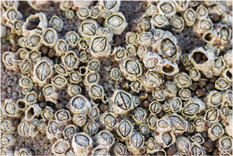
\includegraphics[keepaspectratio]{organisms-that-dont-move/data-image/barnacles.png}}

}

\caption{\label{fig-barnacles}A large number of barnacles fixed to a
rock}

\end{figure}%

\section{Cover-class scales}\label{cover-class-scales}

Three of the most common cover-class scales that you'll come across in
the literature are Braun-Blanquet, Domin and Daubenmire. The simple
approach is to take estimated percentage cover e.g.~within a quadrat,
and map that percentage onto one of these numbered classes. This is good
for long-term monitoring of sites.

\begin{longtable}[t]{lllll}

\caption{\label{tbl-cover-class}Three common cover-class scales seen in
the literature.}

\tabularnewline

\\
\toprule
 & Class & Braun-Blanquet & Domin & Daubenmire\\
\midrule
 & + & <1 \% & Insignif; 1 - 2 inds & \\
 & 1 & 1-5\% & <4\%  - rare & 1 - 5\%\\
 & 2 & 6 - 25\% & < 4\% - occasional & 1 - 5\%\\
 & 3 & 26 - 50\% & <4\% - frequent & 26 - 50\%\\
 & 4 & 51 - 75\% & 4 - 10\% & 51 - 75\%\\
\addlinespace
 & 5 & <75\% & 11 - 25\% & 76 - 95\%\\
 & 6 &  & 26 - 33\% & >96\%\\
 & 7 &  & 34 - 50\% & \\
 & 8 &  & 51 - 75\% & \\
 & 9 &  & 76 - 90\% & \\
\addlinespace
 & 10 &  & >90\% & \\
\bottomrule

\end{longtable}

\section{Quantitative approaches to
sampling}\label{quantitative-approaches-to-sampling}

When you come up with hypotheses you need to test them using statistics.
The qualitative approach will only get you so far and you will need to
use quantitative approaches to get data more suited to statistical
analysis.

What do you measure?

\begin{itemize}
\tightlist
\item
  Individuals:

  \begin{itemize}
  \tightlist
  \item
    Counts of individuals in the experiment area
  \end{itemize}
\item
  Other variables:

  \begin{itemize}
  \item
    Productivity/yield measures, e.g.~total biomass, or harvestable
    yield (seed production, timber volume etc.)
  \item
    Leaf area estimates
  \end{itemize}
\end{itemize}

What you choose depends on the question or hypothesis as well as what
organisms you are interested in.

The most obvious thing to count is the number of individuals at a
particular location, or within a set area. You can then test differences
between areas or within an area through time.

There may be other variables that might be more appropriate and it will,
again, depend on the question. If you're interested in productivity or
`net ecosystem carbon exchange' you might need a biomass measure or a
growth rate, or if it's a measure of fitness then seed production might
be appropriate. If you're creating a life table then the ages, stages or
size of individuals might be appropriate.

Once you've articulated the question you need to think about what data
is appropriate to collect to address it.

Always think about the stats you're going to use before you actually
collect the data. That way you can be sure that you're going to record
appropriate data.

\section{How do you make quantitative
measurements?}\label{how-do-you-make-quantitative-measurements}

We've covered some of what you could measure -- but what about how?

\begin{itemize}
\tightlist
\item
  Density; no. of individuals per unit area

  \begin{itemize}
  \tightlist
  \item
    Comparison among species/treatments
  \end{itemize}
\item
  Frequency; how many occurrences of target in a sample

  \begin{itemize}
  \tightlist
  \item
    Distribution in space
  \end{itemize}
\end{itemize}

The number of individuals counted doesn't give a sense of the area that
you're sampling from. By expressing abundance as density (i.e.~number of
individuals or biomass per, say, square metre) then you have a much more
standardised measure which is therefore appropriate for comparisons
across species, sites or treatments (depending on your question).

Often it's not practical to count all individuals in an area. Instead,
we use sampling. That means counting individuals in small representative
areas and extrapolating. For plants that usually means using quadrats.
For animals it's often by setting traps (physical or camera) which will
generate data from which we determine a frequency of our target species
and get an understanding of their distribution in space.

How many samples to take is an important consideration and you may need
to use some statistical analyses such as power analysis, to work out an
appropriate sampling regime.

Power analysis is best deployed once you've got some pilot data and it
will give you an idea of what sample size would be needed to achieve a
significant result.

There are usually many ways of measuring different properties. Therefore
you should be mindful of the biology of your species when deciding which
one to pick. For example, think about a snail and a slug: they are both
molluscs and quite closely related, but you might not choose the same
size measure for both of them.

\section{Quadrats - The ecologist's
friend}\label{quadrats---the-ecologists-friend}

Quadrats are the `go to' method for sampling plants. They are something
you probably are already familiar with.

Quadrats are squares of known area made of wire or something similar.
There are two types of quadrats (Figure~\ref{fig-quadrats})

\begin{figure}

\begin{minipage}{0.50\linewidth}
\pandocbounded{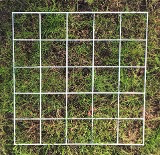
\includegraphics[keepaspectratio]{organisms-that-dont-move/data-image/frame-quadrat.png}}\end{minipage}%
%
\begin{minipage}{0.50\linewidth}
\pandocbounded{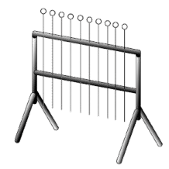
\includegraphics[keepaspectratio]{organisms-that-dont-move/data-image/point-quadrat.png}}\end{minipage}%

\caption{\label{fig-quadrats}A frame quadrat (left) and a point quadrat
(right).}

\end{figure}%

The size and placing of quadrats is determined by the organism \&
hypothesis being tested, and you have to consider the scale of the
organism in relation to the environmental `grain' or `pixel size' you
should be looking at. The most important part of your decision here is
practicality - how many quadrats could you measure? Almost as important
is the size and spread of your organism. You don't want a quadrat that
can only capture one individual. It is a bit like deciding on what sieve
to use -- what mesh size will get you the info you want without getting
a load of excess info that you don't want. That is sometimes hard to
enumerate.

Usually you will only use one quadrat size, but there is potentially
extra information to be gained by using different sizes of quadrats.

As an example, Figure~\ref{fig-daisies-and-dandelions} shows a small
area of a vibrant lawn with a large number of daisies and dandelions.
Here a 1 metre by 1 metre quadrat might be a good size to count
dandelions. However something more like 50 cm by 50 cm (or even smaller)
will be appropriate for counting the daisy flowers. A simple conversion
will allow you to express the density of both flowers to `per square
metre'.

\begin{figure}

\centering{

\pandocbounded{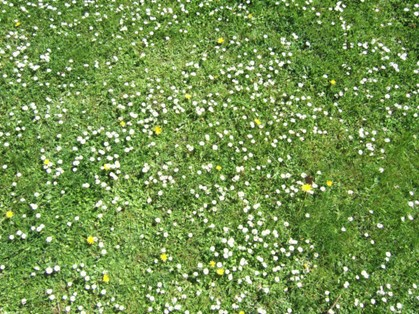
\includegraphics[keepaspectratio]{organisms-that-dont-move/data-image/daisies-and-dandelions.jpg}}

}

\caption{\label{fig-daisies-and-dandelions}}

\end{figure}%

In contrast, in a tropical rainforest
(Figure~\ref{fig-old-growth-rainforest}) a 50 cm quadrat would be
useless. It would be much more likely that you would choose 100m x 100m
(a hectare) to count dipterocarp trees in tropical rainforest, as even
one trunk wouldn't fit into 50cm by 50cm unit space. Trees per hectare
is likely to be much more use than trees per square metre.

\begin{figure}

\centering{

\pandocbounded{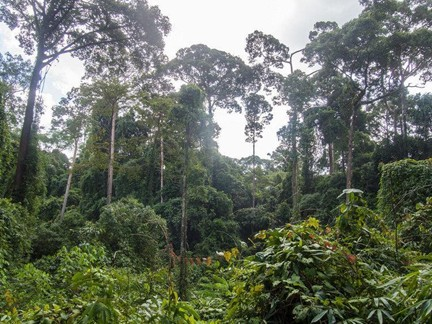
\includegraphics[keepaspectratio]{organisms-that-dont-move/data-image/old-growth-rainforest.jpg}}

}

\caption{\label{fig-old-growth-rainforest}}

\end{figure}%

\section{Placing quadrats}\label{placing-quadrats}

There are lots of ways of placing quadrats and it is not as simple as it
sounds. Throwing quadrats is not recommended as it will nearly always
have a bias of some sort. Instead, consider:

\begin{itemize}
\tightlist
\item
  Random placing:

  \begin{itemize}
  \tightlist
  \item
    Appropriate for most sites and scales
  \item
    Assumes all locations have equal probability of being sampled in
    space and time
  \end{itemize}
\item
  Systematic placing

  \begin{itemize}
  \tightlist
  \item
    Monitoring plots
  \item
    Transects along environmental gradients
  \end{itemize}
\item
  Stratified random sampling

  \begin{itemize}
  \tightlist
  \item
    e.g.~regular samples along randomly placed transects
  \end{itemize}
\end{itemize}

By far the most common approach is to try to achieve random placement
within a larger area. This assumes that all locations have equal
probability of being sampled in space and time so a random sample should
give representative results. Another advantage of random placement of
quadrats is that you can stop when time runs out and there's less bias
than something more systematic.

That being said, systematic sampling is useful too. This is when samples
are structured in time/space. Temporal sampling would be used for
monitoring plots: to be able to return to exactly the same point is
helpful rather than sampling from random locations. One way that is
achieved is to place metal pegs marking quadrat locations and then find
them again using a metal detector. These days, using a GPS on a phone
will get you back to pretty much the exact point.

Sometimes you want to place a sampling transect across an environmental
gradient. That would require systematic placement of quadrats across a
gradient of wet to dry, or open to closed canopy or any other
environmental gradient.

The two approaches could be combined with fixed transects but with
random samples along the transect.

Stratified random sampling is deployed when you know there is some
environmental or habitat change. For example in your wooded area you
know that 70\% has closed canopy and the rest open (clearings, rides,
verges etc.). So to ensure you're sampling from both habitats at the
same density you might place 70\% of the quadrats at random locations in
closed canopy etc.

\chapter{The concept of the individual}\label{sec-individual}

\section{What are we sampling?}\label{what-are-we-sampling}

So far the idea of counting individuals has come up several times.
However, it's not always easy to be sure exactly what an individual is,
or to know whether we've encountered it before. In this module we will
introduce various methods of ecological data collection. Whether we're
interested in distribution, or commonness, or diversity, or function or
fitness, it is important to consider what it is we are actually
sampling, in order to design the right experiment and get useful data.
In a simple world we would address our ecological question by collecting
many independent data points, each being from a genetically distinct
individual, then carry out the appropriate statistical analysis and
decide whether to accept or reject our null hypotheses. But as we are
about to find out, determining what an individual is isn't quite so
straightforward and so the independence of our data points may be called
into question. For example there might be genetic structure in our data.
This has implications for the analysis and interpretation of our data,
and we have to think about how to sample appropriately. In
Figure~\ref{fig-clonal-correlation} there are ten data points, but it
turned out that with clonal growth there are only three genetically
distinct individuals. How should we treat the data when we do an
analysis? Should we assume ten independent data points, or should it be
considered as three independent points?

\begin{figure}

\centering{

\pandocbounded{
\includegraphics[keepaspectratio]{organisms-that-dont-move/organisms-that-dont-move-the-concept-of-the-individual_files/figure-pdf/fig-clonal-correlation-1.pdf}}

}

\caption{\label{fig-clonal-correlation}Ten data points showing a
hypothetical gradient of an unknown variable on the y-axis.}

\end{figure}%

\section{What is an individual?}\label{what-is-an-individual}

When we consider humans, the question of what an individual is seems to
be obvious. We form obvious discrete and genetically distinct units due
to our determinate growth and sexual reproduction
(Figure~\ref{fig-human-life-forms}). Our size and our proportions may
vary over time but our fundamental body plan remains constant. (Let's
not consider identical twins too much here, although we should
acknowledge that they have been an invaluable source of research data
for psychologists.)

\begin{figure}

\centering{

\pandocbounded{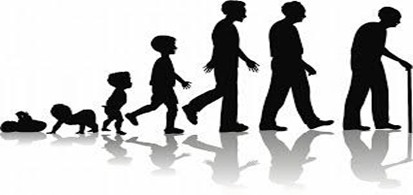
\includegraphics[keepaspectratio]{organisms-that-dont-move/data-image/human-life-forms.jpg}}

}

\caption{\label{fig-human-life-forms}Life forms of a human, from baby
through childhood to adult and older adult.}

\end{figure}%

\section{Individual animals}\label{individual-animals}

Most animals have determinate growth like humans, which means that they
reach a size and stop growing. That is not true for all animals: many
animals, including many fish species, have indeterminate growth, and so
continue to get bigger, the longer they live
(Figure~\ref{fig-big-fish}).

\begin{figure}

\centering{

\pandocbounded{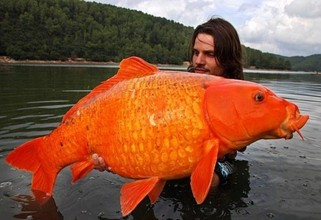
\includegraphics[keepaspectratio]{organisms-that-dont-move/data-image/big-ol-fish.jpg}}

}

\caption{\label{fig-big-fish}A monster koi carp that has continued to
grow as it gets older.}

\end{figure}%

When we are sampling such species, it may make more sense to have some
other measure of abundance rather than just the number of individuals.
The amount of biomass present might be more appropriate, and you will
often see this used for e.g.~marine ecosystems.

The concept of an individual also gets muddy when we consider clonal,
colonial \& social animals where there is strong genetic structure and
differences in ploidy levels. When considering eusocial insects (insects
where some individuals have completely given up with reproduction and
just help raise the offspring of another individual), would it be
appropriate to count organisms or colonies or biomass or number of
reproductive individuals? It really depends upon the question you are
asking. If you are interested in foraging, perhaps data from the
individual ant level would be useful, if you are talking about
colonisation, you probably want data at the nest level.

\section{What is an individual
plant?}\label{what-is-an-individual-plant}

Most plants have indeterminate growth. They keep growing throughout
their lives and will grow in a modular fashion adding stems, leaves and
flowers (Figure~\ref{fig-plant-illustration}).

\begin{itemize}
\tightlist
\item
  Plants are \emph{modular}, growing by increasing the number of units
\item
  Reproduction in plants is variable:

  \begin{itemize}
  \tightlist
  \item
    Sexual: dioecious, hermaphrodite
  \item
    Asexual: apomictic, vegetative
  \end{itemize}
\end{itemize}

\begin{figure}

\centering{

\pandocbounded{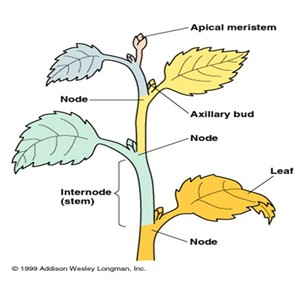
\includegraphics[keepaspectratio]{organisms-that-dont-move/data-image/plant-illustration.jpg}}

}

\caption{\label{fig-plant-illustration}Illustration of a plant showing
the names of various parts of the stem in relation to growth.}

\end{figure}%

Many flowers contain both male and female organs so the individual is a
hermaphrodite. Pollen is akin to sperm and is produced by the male parts
of the flower. However, there are also many species where there are two
separate sexes with individuals producing either only male or female
gametes. In sexual reproduction new individuals are produced by the
fusion of gametes. These gametes can come from different individuals, or
with self fertilization, from the same individual - that is called
`selfing', or `self fertilization'.

There are also plant reproduction strategies that have no fusion of
gametes. This can be vegetative growth where new individuals are
produced through budding or tillering, or it can be by the creation of
seeds without the fusion of gametes which is called apomixis. In some
cases the process requires the presence of pollen to produce the seed,
but no genetic material comes from the pollen.

\section{The Holly and the Ivy}\label{the-holly-and-the-ivy}

To explore the two contrasting methods of sexual reproduction we can use
the Holly (Figure~\ref{fig-holly}) and the Ivy (Figure~\ref{fig-ivy}).

\begin{figure}

\centering{

\pandocbounded{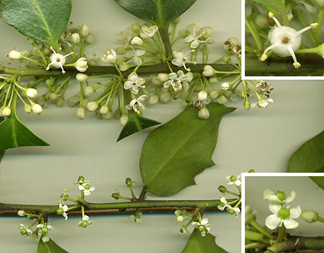
\includegraphics[keepaspectratio]{organisms-that-dont-move/data-image/holly-leaves-and-flowers.png}}

}

\caption{\label{fig-holly}}

\end{figure}%

Holly (\emph{Ilex aquifolium}) is dioecious: it has male and female
flowers on separate plants. Male plants have staminate (male,
pollen-producing) flowers with anthers and stamen
(Figure~\ref{fig-holly}). Female plants have carpellate (female,
ovule-producing) flowers. When you see holly with berries on, you know
it's a female plant. Holly has to undergo sexual reproduction -- it
cannot self fertilize because it only has male or female reproductive
parts on a single plant. Therefore each individual is a genetically
distinct individual.

\begin{figure}

\centering{

\pandocbounded{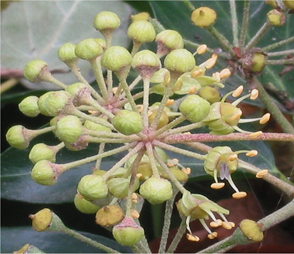
\includegraphics[keepaspectratio]{organisms-that-dont-move/data-image/ivy-flowers.png}}

}

\caption{\label{fig-ivy}}

\end{figure}%

Ivy (\emph{Hedera helix}) is not so simple. This species is
hermaphrodite with male and female parts on the same flower
(Figure~\ref{fig-ivy}; it is like the classic flower diagram with
sepals, petals, carpels and stamen all in one flower). Seeds are formed
after fusion of gametes, but self fertilization is possible. Ivy also
does a lot of vegetative growth -- if it grows along the ground and
where nodes touch the ground they form rootlets. Individuals could
therefore be clonal (if vegetative), genetically identical to the
parent, or be genetically mixed with both gametes coming from the same
parent (if selfing) or genetically distinct (if from out-crossing).

\section{Asexual reproduction:
vegetative}\label{asexual-reproduction-vegetative}

There are some extreme cases where vegetative reproduction completely
dominates. Enter Pando the trembling giant -- this single male clone of
quaking aspen (\emph{Populus tremuloides}) in Utah has been around for
many thousands of years and consists of roots and c.~47,000 stems
covering a huge area (43 hectares; Figure~\ref{fig-pando}). It is
difficult to count individuals where they are connected vegetative
clones. Is this one individual or 47,000? Go and read about
\href{https://en.wikipedia.org/wiki/Pando_(tree)}{Pando the trembling
giant} and the factors that gave rise to it! It is fascinating stuff.

\begin{figure}

\centering{

\pandocbounded{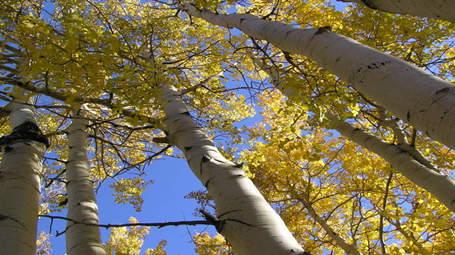
\includegraphics[keepaspectratio]{organisms-that-dont-move/data-image/pando-the-trembling-giant.png}}

}

\caption{\label{fig-pando}}

\end{figure}%

\section{Asexual reproduction:
apomixis}\label{asexual-reproduction-apomixis}

The other type of asexual reproduction we find in plants is exemplified
in the asteraceae family (e.g.~dandelion) and Rosaceae family
(e.g.~bramble). These reproduce asexually through apomixis, or
specifically agamospermy, in which seeds are produced without meiosis.
In some parts of the range there is normal sexual reproduction with
fusion of gametes. But at northern latitudes, such as the British Isles,
there is only apomixis, so the seeds on a dandelion clock
(Figure~\ref{fig-dandelion}) are genetically identical. But they are not
genetically identical to the seeds on another plant (unless the two
plants are clones). They don't interbreed, so there are a number of
genetic lines with no recombination between them. This goes against the
definition of a species (not all individuals are capable of
interbreeding) so we call these aggregated species. Again, we must
consider what an individual is. If we are just counting organisms and
investigating their distribution, treating each plant as an individual
is probably fine. If we are asking a question about fitness, genetic
relatedness may play a part so what do we consider the individual to be
then?

\begin{figure}

\centering{

\pandocbounded{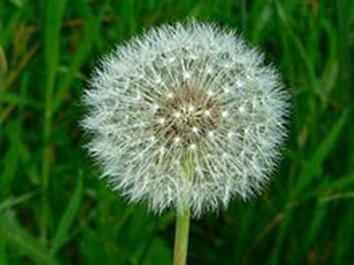
\includegraphics[keepaspectratio]{organisms-that-dont-move/data-image/common-dandelion.jpg}}

}

\caption{\label{fig-dandelion}}

\end{figure}%

\section{Fungal populations}\label{fungal-populations}

Sampling fungal populations suffers from many of the challenges
mentioned previously, including indeterminate growth and varied
reproductive strategies. An added complication is that for most of their
life cycle they are not visible to us. Only when sporocarp (or fruiting
body in the form of mushrooms, toadstools, puff-balls etc.) is produced
can we visibly see fungi (Figure~\ref{fig-fungus}).

\begin{figure}

\centering{

\pandocbounded{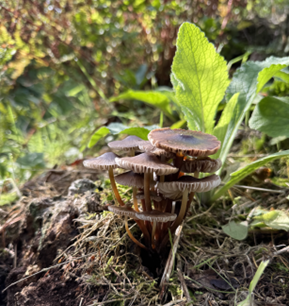
\includegraphics[keepaspectratio]{organisms-that-dont-move/data-image/fungal-fruiting-body.png}}

}

\caption{\label{fig-fungus}}

\end{figure}%

Just counting the fruiting bodies is not a great way to sample abundance
of fungi. It is very biased as they are around for different lengths of
time, highly variable within and between years. This might be true even
when there is little difference in the amount of mycelium; this is the
part of the organism that does everything except reproduction, and we're
not counting it! New indirect methods have much improved fungal sampling
such as testing for the presence of fungal DNA/RNA in the field from
samples of soil.

\chapter{The R code}\label{sec-poisson-r-code}

\section{Plantago data}\label{plantago-data}

\subsection{Introduction to the worked
example}\label{introduction-to-the-worked-example}

In the practical (Chapter~\ref{sec-plantago-practical}), you
investigated the distribution of populations of ribwort plantain
(\emph{Plantago lanceolata}) in a specific area of campus.

You used quadrats of two different sizes - 100cm x 100cm (large) and
40cm x 40cm (small) to determine the impacts that sampling efforts has
on your findings.

You then entered your data onto the shared Google sheet.

In this worked example, we will consider the 2025 data from the Plantago
datasheet.

First, you'll need to run the relevant packages and read in the data
from the practical. We're using Google sheets to store the data; you can
use the \texttt{googlesheets4} package to read in from a google sheets
document by extracting the unique code contained in the URL (see
Figure~\ref{fig-google-sheets-url}). For this example, we're going to
work with the 2025 data, so the results for your data \textbf{will} look
different.

\begin{figure}

\centering{

\pandocbounded{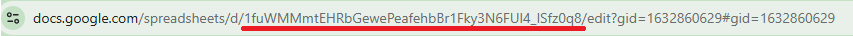
\includegraphics[keepaspectratio]{organisms-that-dont-move/data-image/url-screenshot.png}}

}

\caption{\label{fig-google-sheets-url}The underlined section is the
unique identifier for this google sheet. You can copy and paste that
into the code below, and update the `sheet' command to reflect the year
you want.}

\end{figure}%

\subsection{Data import}\label{data-import}

\begin{Shaded}
\begin{Highlighting}[]
\FunctionTok{library}\NormalTok{(tidyverse)}
\FunctionTok{library}\NormalTok{(googlesheets4)}

\CommentTok{\# Data Import}

\CommentTok{\# Disable authentication since the sheet is publicly viewable}
\FunctionTok{gs4\_deauth}\NormalTok{()}

\CommentTok{\# Read in the data from Google Sheets — update the sheet name to}
\CommentTok{\# match the survey year you want to analyse}
\CommentTok{\# If you\textquotesingle{}re using your own data from your own google sheet, update the }
\CommentTok{\# unique sheet identifier}
\NormalTok{plantago\_data }\OtherTok{\textless{}{-}} \FunctionTok{read\_sheet}\NormalTok{(}\StringTok{"1fuWMMmtEHRbGewePeafehbBr1Fky3N6FUI4\_ISfz0q8"}\NormalTok{,}
  \AttributeTok{sheet =} \StringTok{"2025"}\NormalTok{) }\SpecialCharTok{|\textgreater{}}
\NormalTok{  janitor}\SpecialCharTok{::}\FunctionTok{clean\_names}\NormalTok{()}

\CommentTok{\# Sanity check: inspect the first few rows to confirm import worked}
\FunctionTok{head}\NormalTok{(plantago\_data)}
\end{Highlighting}
\end{Shaded}

\begin{verbatim}
# A tibble: 6 x 5
  sampler_id     x     y quadrat_size num_of_individuals
  <chr>      <dbl> <dbl> <chr>                     <dbl>
1 Gadwall        1    14 S                             0
2 Gadwall        1    14 L                             5
3 Gadwall        3    13 S                             0
4 Gadwall        3    13 L                             0
5 Gadwall       12     6 S                             0
6 Gadwall       12     6 L                             3
\end{verbatim}

As this is a sheet that gets updated every year by each student cohort,
the terms used for the small and large quadrat in the column
``quadrat\_size'' may differ. For 2025, these are S and L.

\subsection{Data preparation}\label{data-preparation}

Now we need to prepare the data. For this analysis, we're going to use
the large quadrats.

\begin{Shaded}
\begin{Highlighting}[]
\CommentTok{\# Keep only large quadrats for this analysis}
\NormalTok{large\_quad }\OtherTok{\textless{}{-}}\NormalTok{ plantago\_data }\SpecialCharTok{|\textgreater{}}
  \FunctionTok{filter}\NormalTok{(quadrat\_size }\SpecialCharTok{==} \StringTok{"L"}\NormalTok{)}

\CommentTok{\# Count the number of quadrats with each observed individual count}
\NormalTok{large\_quad\_summary }\OtherTok{\textless{}{-}}\NormalTok{ large\_quad }\SpecialCharTok{|\textgreater{}}
  \FunctionTok{group\_by}\NormalTok{(num\_of\_individuals) }\SpecialCharTok{|\textgreater{}}
  \FunctionTok{summarise}\NormalTok{(}\AttributeTok{observed =} \FunctionTok{length}\NormalTok{(num\_of\_individuals))}

\CommentTok{\# Quick visual check of the distribution}
\FunctionTok{ggplot}\NormalTok{(}\AttributeTok{data =}\NormalTok{ large\_quad, }\FunctionTok{aes}\NormalTok{(}\AttributeTok{x =}\NormalTok{ num\_of\_individuals)) }\SpecialCharTok{+}
  \FunctionTok{geom\_bar}\NormalTok{()}
\end{Highlighting}
\end{Shaded}

\pandocbounded{
\includegraphics[keepaspectratio]{organisms-that-dont-move/organisms-that-dont-move-poisson-r-code_files/figure-pdf/unnamed-chunk-3-1.pdf}}

What can we see about the distribution of our data? There are a large
number of quadrats that contain 0 individuals or 1 individuals, followed
by a long tail of quadrats that contain higher numbers of individuals.

Does this match what we would expect?

Next, we need to use this data to generated our \emph{expected} number
of quadrats that contain that number of individuals based on the poisson
distribution. Based on the mean number of plants per quadrat, how many
quadrats out of our total number of samples do we expect to contain 0,
1, 2, 3\ldots, etc individuals.

\subsection{Poisson parameters}\label{poisson-parameters}

\begin{Shaded}
\begin{Highlighting}[]
\CommentTok{\# For a Poisson distribution, mean ≈ variance; compare these to}
\CommentTok{\# check fit}
\NormalTok{mean }\OtherTok{\textless{}{-}} \FunctionTok{mean}\NormalTok{(large\_quad}\SpecialCharTok{$}\NormalTok{num\_of\_individuals)}
\NormalTok{variance }\OtherTok{\textless{}{-}} \FunctionTok{var}\NormalTok{(large\_quad}\SpecialCharTok{$}\NormalTok{num\_of\_individuals)}

\NormalTok{total\_plants }\OtherTok{\textless{}{-}} \FunctionTok{sum}\NormalTok{(large\_quad}\SpecialCharTok{$}\NormalTok{num\_of\_individuals)}
\NormalTok{total\_quads }\OtherTok{\textless{}{-}} \FunctionTok{length}\NormalTok{(large\_quad}\SpecialCharTok{$}\NormalTok{num\_of\_individuals)}

\CommentTok{\# Calculate the expected number of quadrats for each count under}
\CommentTok{\# a Poisson distribution with lambda = sample mean}
\NormalTok{large\_quad\_summary }\OtherTok{\textless{}{-}}\NormalTok{ large\_quad\_summary }\SpecialCharTok{|\textgreater{}}
  \FunctionTok{mutate}\NormalTok{(}\AttributeTok{expected =} \FunctionTok{dpois}\NormalTok{(num\_of\_individuals, }\AttributeTok{lambda =}\NormalTok{ mean) }\SpecialCharTok{*}
\NormalTok{           total\_quads)}
\end{Highlighting}
\end{Shaded}

We have now generated a new column in our dataset that shows the
expected number of quadrats containing that number of individuals using
the poisson distribution.

However, the Chi-squared (\(\chi^2\)) test makes a few assumptions that
we now need to check before we proceed with the statistical testing.

\subsection{Chi-squared validity}\label{chi-squared-validity}

The Chi-squared test requires expected values of ≥ 1 in each cell. When
it comes to your data, you will need to now look at the generated table
and determine where you see expected values of \textless{} 1; is it at
the high end, the low end, or both ends of your data?

Where expected counts are too small, we collapse neighbouring
categories. For example, if the expected value of the number of quadrats
containing 11 individuals is below 1, we then collapse the data into
``10 or more'' individuals.

You may need to apply either or both of the following processes. For our
2025 data, you will need to do both.

\subsubsection{Low end}\label{low-end}

The following code generates a value for the `low cutoff' category. For
the 2025 data, you can see that the expected number of quadrats with 0
individuals is 3.20 x \(10\^{-1}\), while the expected number of
quadrats with 1 individual is 1.68.

\begin{Shaded}
\begin{Highlighting}[]
\CommentTok{\# Inspect large\_quad\_summary to find where expected counts drop}
\CommentTok{\# below 1 at the low end, then set low\_cutoff to the last}
\CommentTok{\# affected count. e.g. low\_cutoff = 1 collapses counts 0 and 1}
\CommentTok{\# into a single "≤ 1" category.}
\NormalTok{low\_cutoff }\OtherTok{\textless{}{-}} \DecValTok{1} \CommentTok{\# You might need to change this based on your data}

\NormalTok{large\_quad\_low }\OtherTok{\textless{}{-}}\NormalTok{ large\_quad\_summary }\SpecialCharTok{|\textgreater{}}
  \FunctionTok{filter}\NormalTok{(num\_of\_individuals }\SpecialCharTok{\textless{}=}\NormalTok{ low\_cutoff) }\SpecialCharTok{|\textgreater{}}
  \FunctionTok{summarise}\NormalTok{(}\AttributeTok{num\_of\_individuals =}\NormalTok{ low\_cutoff,}
            \AttributeTok{observed =} \FunctionTok{sum}\NormalTok{(observed),}
            \AttributeTok{expected =} \FunctionTok{sum}\NormalTok{(expected))}
\end{Highlighting}
\end{Shaded}

\subsubsection{High end}\label{high-end}

The following code generates a value for the `high cutoff' category. For
the 2025 data, you can see that the expected number of quadrats with 10
individuals is 1.54, while the expected number of quadrats with 11
individuals is 7.39 x \(10^{-1}\).

\begin{Shaded}
\begin{Highlighting}[]
\CommentTok{\# Similarly, collapse the sparse high{-}count tail into a single}
\CommentTok{\# "≥ high\_cutoff" category. The expected value uses the Poisson}
\CommentTok{\# survival function so it accounts for all counts from}
\CommentTok{\# high\_cutoff to infinity, not just those observed.}
\CommentTok{\# e.g. high\_cutoff = 10 collapses counts 10, 11, 12, … into one}
\CommentTok{\# category.}
\NormalTok{high\_cutoff }\OtherTok{\textless{}{-}} \DecValTok{10} \CommentTok{\# You might need to change this based on your data}

\NormalTok{large\_quad\_high }\OtherTok{\textless{}{-}}\NormalTok{ large\_quad\_summary }\SpecialCharTok{|\textgreater{}}
  \FunctionTok{filter}\NormalTok{(num\_of\_individuals }\SpecialCharTok{\textgreater{}=}\NormalTok{ high\_cutoff) }\SpecialCharTok{|\textgreater{}}
  \FunctionTok{summarise}\NormalTok{(}\AttributeTok{num\_of\_individuals =}\NormalTok{ high\_cutoff,}
            \AttributeTok{observed =} \FunctionTok{sum}\NormalTok{(observed),}
            \AttributeTok{expected =}\NormalTok{ (}\DecValTok{1} \SpecialCharTok{{-}} \FunctionTok{ppois}\NormalTok{(}\DecValTok{10}\NormalTok{, }\AttributeTok{lambda =}\NormalTok{ mean)) }\SpecialCharTok{*}\NormalTok{ total\_quads)}
\end{Highlighting}
\end{Shaded}

\subsubsection{Bind the categories with the rest of the
data}\label{bind-the-categories-with-the-rest-of-the-data}

We then need to combine the collapsed categories with the untouched
middle counts (\textgreater1 and \textless10). You will need to alter
this code depending on which cutoff points you had to create; if you did
not need to create a low cutoff point, you can exclude that command from
your data.

\begin{Shaded}
\begin{Highlighting}[]
\CommentTok{\# Bind the collapsed low and high categories with the untouched}
\CommentTok{\# middle counts}
\NormalTok{large\_quad\_summary\_comb }\OtherTok{\textless{}{-}}\NormalTok{ large\_quad\_summary }\SpecialCharTok{|\textgreater{}}
  \FunctionTok{filter}\NormalTok{(num\_of\_individuals }\SpecialCharTok{\textgreater{}}\NormalTok{ low\_cutoff,}
\NormalTok{         num\_of\_individuals }\SpecialCharTok{\textless{}}\NormalTok{ high\_cutoff) }\SpecialCharTok{|\textgreater{}}
  \FunctionTok{bind\_rows}\NormalTok{(large\_quad\_low, large\_quad\_high) }\SpecialCharTok{|\textgreater{}}
  \FunctionTok{arrange}\NormalTok{(num\_of\_individuals)}
\end{Highlighting}
\end{Shaded}

You can see from the table that the number of quadrats with the observed
number of individuals pools the 0 and 1 categories, and the categories
for 10 or more individuals.

\subsection{The Chi-squared test}\label{the-chi-squared-test}

Remember the chi-squared equation? (Hint: check
Chapter~\ref{sec-poisson} if you don't!)

\[
\chi^2 = \sum{(O - E)^2 \over E}
\] We can now use this format to calcuate the chi squared statistic, and
work out the \emph{P} value that that represents

\begin{Shaded}
\begin{Highlighting}[]
\CommentTok{\# Compute each category\textquotesingle{}s contribution to the chi{-}squared}
\CommentTok{\# statistic}
\NormalTok{large\_quad\_summary\_comb }\OtherTok{\textless{}{-}}\NormalTok{ large\_quad\_summary\_comb }\SpecialCharTok{|\textgreater{}}
  \FunctionTok{mutate}\NormalTok{(}\AttributeTok{chi\_sq =}\NormalTok{ ((observed }\SpecialCharTok{{-}}\NormalTok{ expected)}\SpecialCharTok{\^{}}\DecValTok{2}\NormalTok{) }\SpecialCharTok{/}\NormalTok{ expected)}

\NormalTok{chi\_sq\_statistic }\OtherTok{\textless{}{-}} \FunctionTok{sum}\NormalTok{(large\_quad\_summary\_comb}\SpecialCharTok{$}\NormalTok{chi\_sq)}

\CommentTok{\# Degrees of freedom = number of categories − 1 (for the test)}
\CommentTok{\# − 1 (for the estimated parameter: the mean/lambda)}
\NormalTok{degrees\_of\_freedom }\OtherTok{\textless{}{-}} \FunctionTok{nrow}\NormalTok{(large\_quad\_summary\_comb) }\SpecialCharTok{{-}} \DecValTok{1} \SpecialCharTok{{-}} \DecValTok{1}

\CommentTok{\# P{-}value: probability of observing a chi{-}squared statistic this}
\CommentTok{\# large or larger under the null hypothesis that counts follow a}
\CommentTok{\# Poisson distribution}
\FunctionTok{pchisq}\NormalTok{(chi\_sq\_statistic, }\AttributeTok{df =}\NormalTok{ degrees\_of\_freedom,}
       \AttributeTok{lower.tail =} \ConstantTok{FALSE}\NormalTok{)}
\end{Highlighting}
\end{Shaded}

\begin{verbatim}
[1] 3.492703e-54
\end{verbatim}

What can we conclude here? Is our data significantly different to the
poisson distribution (i.e.~randomly distributed)?

And by comparing the mean to the variance (hint: check
Chapter~\ref{sec-poisson} here as a reminder), do we think that the
distribution of this plant is clustered or overdispersed?

\subsection{Figure of observed and expected
values}\label{figure-of-observed-and-expected-values}

Finally, we can create a plot to visuliase our generated expected values
using the poisson distribution, and our observed dataset

\begin{Shaded}
\begin{Highlighting}[]
\FunctionTok{ggplot}\NormalTok{(large\_quad\_summary\_comb, }\FunctionTok{aes}\NormalTok{(}\AttributeTok{x =}\NormalTok{ num\_of\_individuals)) }\SpecialCharTok{+}
  \FunctionTok{geom\_col}\NormalTok{(}\FunctionTok{aes}\NormalTok{(}\AttributeTok{y =}\NormalTok{ observed)) }\SpecialCharTok{+}
  \FunctionTok{geom\_point}\NormalTok{(}\FunctionTok{aes}\NormalTok{(}\AttributeTok{y =}\NormalTok{ expected), }
             \AttributeTok{color =} \StringTok{"red"}\NormalTok{, }\AttributeTok{size =} \DecValTok{5}\NormalTok{, }\AttributeTok{pch =} \DecValTok{20}\NormalTok{) }\SpecialCharTok{+}
  \CommentTok{\# You might need to change breaks and labels based on your data}
  \FunctionTok{scale\_x\_continuous}\NormalTok{(}\AttributeTok{breaks =} \FunctionTok{seq}\NormalTok{(}\DecValTok{1}\NormalTok{, }\DecValTok{10}\NormalTok{, }\AttributeTok{by =} \DecValTok{1}\NormalTok{),}
                     \AttributeTok{name =} \StringTok{"Number of individuals per quadrat"}\NormalTok{,}
                     \AttributeTok{labels =} \FunctionTok{c}\NormalTok{(}\StringTok{"0 or 1"}\NormalTok{, }\DecValTok{2}\SpecialCharTok{:}\DecValTok{9}\NormalTok{, }\StringTok{"10 or above"}\NormalTok{)) }\SpecialCharTok{+}
  \FunctionTok{scale\_y\_continuous}\NormalTok{(}\AttributeTok{name =} \StringTok{"Number of quadrats}\SpecialCharTok{\textbackslash{}n}\StringTok{(bars = observed, dots = expected)"}\NormalTok{,}
                     \AttributeTok{expand =} \FunctionTok{c}\NormalTok{(}\DecValTok{0}\NormalTok{, }\DecValTok{0}\NormalTok{)) }\SpecialCharTok{+}
  \FunctionTok{theme\_classic}\NormalTok{() }
\end{Highlighting}
\end{Shaded}

\pandocbounded{
\includegraphics[keepaspectratio]{organisms-that-dont-move/organisms-that-dont-move-poisson-r-code_files/figure-pdf/unnamed-chunk-9-1.pdf}}

\subsection{Task: your turn!}\label{task-your-turn}

Try running the code again using the small size quadrats rather than the
large quadrats. What changes? What can we start to conclude about the
importance of sampling effort on the poisson distribute?

Try running the code again using a different year of study. At what
point do you need to collapse your categories? Again, what changes
between the large and small quadrats?

\chapter{\texorpdfstring{The workshop: \emph{Plantago} and
LEGO}{The workshop: Plantago and LEGO}}\label{sec-lego-workshop}

\section{\texorpdfstring{\emph{Plantago}}{Plantago}}\label{plantago}

If you haven't already, read through Chapter~\ref{sec-poisson-r-code}.
This walks you through some example data from 2025, including how to
upload the data and how to collapse categories when your expected values
for the number of individuals per quadrat are less than one.

Have a go now at working through that process with this year's plantago
data. Which categories do you need to collapse? Is there a difference
between \emph{P} value generated for the large and the small categories
of quadrat?

\section{LEGO}\label{lego}

Next, we'll sample your LEGO communities. Again, there will be a worked
example using model data. Then, you can sample your own communities
(using whatever category you have developed for a `species') and try it
yourself.

\subsection{Loading in the data}\label{loading-in-the-data}

For this example, we are using the data contained in the
\href{https://docs.google.com/spreadsheets/d/1zEzeLF_fLPYlXqvPcCZ0r0Jmb_i7pkLywQs--5LQuZw/edit?gid=0\#gid=0}{36i
model data}. Follow the process through, then try it yourself with your
own data.

In this scenario, we have a spreadsheet documenting 6 samples, where we
counted the number of red, blue, green, and yellow `plants'.

\begin{Shaded}
\begin{Highlighting}[]
\CommentTok{\# load the googlesheets function (if you haven\textquotesingle{}t already)}
\FunctionTok{library}\NormalTok{(googlesheets4)}
\CommentTok{\# load tidyverse (if you haven\textquotesingle{}t already)}
\FunctionTok{library}\NormalTok{(tidyverse)}

\CommentTok{\# turn off authentication (because the sheet is viewable by anyone)}
\FunctionTok{gs4\_deauth}\NormalTok{() }

\CommentTok{\# Read in the data from Google Sheets — update the sheet name to}
\CommentTok{\# match the survey year you want to analyse}
\CommentTok{\# If you\textquotesingle{}re using your own data from your own google sheet, update the }
\CommentTok{\# unique sheet identifier}
\CommentTok{\# Leave as it is to proceed with the example data}
\NormalTok{community\_data }\OtherTok{\textless{}{-}} \FunctionTok{read\_sheet}\NormalTok{(}\StringTok{"1zEzeLF\_fLPYlXqvPcCZ0r0Jmb\_i7pkLywQs{-}{-}5LQuZw"}\NormalTok{,}
                             \AttributeTok{sheet =} \StringTok{"PlantSamples"}\NormalTok{) }\SpecialCharTok{|\textgreater{}}
\NormalTok{  janitor}\SpecialCharTok{::}\FunctionTok{clean\_names}\NormalTok{()}

 \CommentTok{\# check the top of the spreadsheet to make sure it worked}
\FunctionTok{head}\NormalTok{(community\_data)}
\end{Highlighting}
\end{Shaded}

\begin{verbatim}
# A tibble: 6 x 5
  sample   red  blue green yellow
   <dbl> <dbl> <dbl> <dbl>  <dbl>
1      1     0     5     2      1
2      2     1     4     2      1
3      3     1     5     0      2
4      4     0     4     2      2
5      5     1     5     1      1
6      6     0     5     1      2
\end{verbatim}

\subsection{Calculating the fraction of the population occupied by the
dominant taxon from one
sample}\label{calculating-the-fraction-of-the-population-occupied-by-the-dominant-taxon-from-one-sample}

Lets say you've pulled 6 LEGO bricks out of your bag, and we're
interested in a taxon of Blue bricks. Maybe we already know this is
likely the dominant taxon based on other existing literature or
observations made in this area.

\begin{Shaded}
\begin{Highlighting}[]
\CommentTok{\# The number of bricks you pulled out of your back gives you the sample size}
\NormalTok{sample\_size }\OtherTok{\textless{}{-}} \DecValTok{6} 

\CommentTok{\#The number of those bricks that are from the dominant taxon}
\NormalTok{sample\_number\_dominant\_individuals }\OtherTok{\textless{}{-}} \DecValTok{1} 

\CommentTok{\# The fraction or proportion of the sample that is the dominant taxon}
\NormalTok{sample\_dominant\_fraction }\OtherTok{\textless{}{-}}\NormalTok{ sample\_number\_dominant\_individuals}\SpecialCharTok{/}\NormalTok{sample\_size}

\CommentTok{\#display the value }
\FunctionTok{print}\NormalTok{(sample\_dominant\_fraction)}
\end{Highlighting}
\end{Shaded}

\begin{verbatim}
[1] 0.1666667
\end{verbatim}

\subsection{Calculating the fraction of the population occupied by the
dominant taxon from multiple
samples}\label{calculating-the-fraction-of-the-population-occupied-by-the-dominant-taxon-from-multiple-samples}

We need to know how many samples we've taken later on, but we also need
to sum the total number of individuals per sample. The code below drops
the first row (`Sample'), but sums the number of individuals

\begin{Shaded}
\begin{Highlighting}[]
\CommentTok{\# Create a community data object selecting only the lego colours}
\CommentTok{\# Note that we are overwriting the original community\_data object with this new mutated version}
\NormalTok{community\_data }\OtherTok{\textless{}{-}}\NormalTok{ community\_data }\SpecialCharTok{|\textgreater{}}
  \FunctionTok{mutate}\NormalTok{(}\StringTok{"Total"} \OtherTok{=} \FunctionTok{rowSums}\NormalTok{(community\_data[,}\SpecialCharTok{{-}}\DecValTok{1}\NormalTok{]))}
\end{Highlighting}
\end{Shaded}

Assuming we are interested in the blue lego species, we can calculate
the cumulative sum of the sample size, and the number of blue
individuals from samples 1, 1+2, 1+2+3, \ldots{} etc. We can then find
the relative proportion of the number of blue individuals to the total
number of all individuals.

\begin{Shaded}
\begin{Highlighting}[]
\NormalTok{cumulative\_total }\OtherTok{\textless{}{-}} \FunctionTok{cumsum}\NormalTok{(community\_data}\SpecialCharTok{$}\NormalTok{Total)}
\NormalTok{cumulative\_blue }\OtherTok{\textless{}{-}} \FunctionTok{cumsum}\NormalTok{(community\_data}\SpecialCharTok{$}\NormalTok{blue)}
\NormalTok{proportion\_blue }\OtherTok{\textless{}{-}}\NormalTok{ cumulative\_blue}\SpecialCharTok{/}\NormalTok{cumulative\_total}
\end{Highlighting}
\end{Shaded}

Next, we need to plot the fraction of blue to total individuals against
sample size.

Notice that in this ggplot code, we're not specifying
\texttt{data\ =\ community\_data}; this is because we're using the
object \texttt{proportion\_blue} that we created above on our y axis,
which is not contained in the dataset.

We can still call the \texttt{sample} column from
\texttt{community\_data} using the \texttt{\$} notation.

\begin{Shaded}
\begin{Highlighting}[]
\FunctionTok{ggplot}\NormalTok{() }\SpecialCharTok{+}
  \FunctionTok{geom\_point}\NormalTok{(}\FunctionTok{aes}\NormalTok{(}\AttributeTok{x =}\NormalTok{ community\_data}\SpecialCharTok{$}\NormalTok{sample, }\AttributeTok{y =}\NormalTok{ proportion\_blue)) }\SpecialCharTok{+} 
  \FunctionTok{scale\_x\_discrete}\NormalTok{(}\AttributeTok{name =} \StringTok{"Cumulative number of samples"}\NormalTok{) }\SpecialCharTok{+} 
  \FunctionTok{scale\_y\_continuous}\NormalTok{(}\AttributeTok{name =} \StringTok{"Proportion blue"}\NormalTok{,}
                   \AttributeTok{expand =} \FunctionTok{c}\NormalTok{(}\DecValTok{0}\NormalTok{,}\DecValTok{0}\NormalTok{),}
                   \AttributeTok{limits =} \FunctionTok{c}\NormalTok{(}\FloatTok{0.5}\NormalTok{,}\FloatTok{0.7}\NormalTok{)) }\SpecialCharTok{+} 
  \FunctionTok{theme\_bw}\NormalTok{()}
\end{Highlighting}
\end{Shaded}

\pandocbounded{
\includegraphics[keepaspectratio]{organisms-that-dont-move/organisms-that-dont-move-workshop-ver-2_files/figure-pdf/unnamed-chunk-5-1.pdf}}

\subsection{Applying the Poisson distribution test to our lego
data}\label{applying-the-poisson-distribution-test-to-our-lego-data}

We're still interested in the distribution of our blue individuals. In
this section, we're going to see if the distribution of the blue
individuals differs from the Poisson distribution.

\begin{Shaded}
\begin{Highlighting}[]
\CommentTok{\# Keep only blue individuals for this analysis, and rename the column to }
\CommentTok{\# something more descriptive}
\NormalTok{blue\_lego }\OtherTok{\textless{}{-}}\NormalTok{ community\_data }\SpecialCharTok{|\textgreater{}}
  \FunctionTok{select}\NormalTok{(blue) }\SpecialCharTok{|\textgreater{}}
  \FunctionTok{rename}\NormalTok{(}\AttributeTok{number\_of\_individuals =}\NormalTok{ blue)}

\CommentTok{\# Count the number of samples with each observed individual count}
\NormalTok{blue\_lego\_summary }\OtherTok{\textless{}{-}}\NormalTok{ blue\_lego }\SpecialCharTok{|\textgreater{}}
  \FunctionTok{group\_by}\NormalTok{(number\_of\_individuals) }\SpecialCharTok{|\textgreater{}}
  \FunctionTok{summarise}\NormalTok{(}\AttributeTok{observed =} \FunctionTok{length}\NormalTok{(number\_of\_individuals))}

\CommentTok{\# Quick visual check of the distribution}
\FunctionTok{ggplot}\NormalTok{(}\AttributeTok{data =}\NormalTok{ blue\_lego, }\FunctionTok{aes}\NormalTok{(}\AttributeTok{x =}\NormalTok{ number\_of\_individuals)) }\SpecialCharTok{+}
  \FunctionTok{geom\_bar}\NormalTok{()}
\end{Highlighting}
\end{Shaded}

\pandocbounded{
\includegraphics[keepaspectratio]{organisms-that-dont-move/organisms-that-dont-move-workshop-ver-2_files/figure-pdf/unnamed-chunk-6-1.pdf}}

Looking at our model data, we have no quadrats with zero individuals,
two quadrats with 4 individuals, and four quadrats with 5 individuals.

Does this match what we would expect?

Next, we need to use this data to generated our \emph{expected} number
of quadrats that contain that number of individuals based on the poisson
distribution. Based on the mean number of blue lego pieces per sample,
how many samples do we expect to contain 4 or 5 individuals?

\subsection{Poisson parameters}\label{poisson-parameters-1}

\begin{Shaded}
\begin{Highlighting}[]
\CommentTok{\# For a Poisson distribution, mean ≈ variance; compare these to}
\CommentTok{\# check fit}
\NormalTok{mean }\OtherTok{\textless{}{-}} \FunctionTok{mean}\NormalTok{(blue\_lego}\SpecialCharTok{$}\NormalTok{number\_of\_individuals)}
\NormalTok{variance }\OtherTok{\textless{}{-}} \FunctionTok{var}\NormalTok{(blue\_lego}\SpecialCharTok{$}\NormalTok{number\_of\_individuals)}

\NormalTok{total\_blue }\OtherTok{\textless{}{-}} \FunctionTok{sum}\NormalTok{(blue\_lego}\SpecialCharTok{$}\NormalTok{number\_of\_individuals)}
\NormalTok{total\_samples }\OtherTok{\textless{}{-}} \FunctionTok{length}\NormalTok{(blue\_lego}\SpecialCharTok{$}\NormalTok{number\_of\_individuals)}

\CommentTok{\# Calculate the expected number of quadrats for each count under}
\CommentTok{\# a Poisson distribution with lambda = sample mean}
\NormalTok{blue\_lego\_summary }\OtherTok{\textless{}{-}}\NormalTok{ blue\_lego\_summary }\SpecialCharTok{|\textgreater{}}
  \FunctionTok{mutate}\NormalTok{(}\AttributeTok{expected =} \FunctionTok{dpois}\NormalTok{(number\_of\_individuals, }\AttributeTok{lambda =}\NormalTok{ mean) }\SpecialCharTok{*}
\NormalTok{           total\_samples)}
\end{Highlighting}
\end{Shaded}

We have now generated a new column in our dataset that shows the
expected number of quadrats containing that number of individuals using
the poisson distribution.

Unlike in our example \emph{plantago} data
(Chapter~\ref{sec-poisson-r-code}), we do not need to collapse any
categories, as our predicted values are both greater than 1 in each
category.

Lets calculate the Chi-squared value, and determine the \emph{P} value:

\begin{Shaded}
\begin{Highlighting}[]
\CommentTok{\# Compute each category\textquotesingle{}s contribution to the chi{-}squared}
\CommentTok{\# statistic}
\NormalTok{blue\_lego\_summary }\OtherTok{\textless{}{-}}\NormalTok{ blue\_lego\_summary }\SpecialCharTok{|\textgreater{}}
  \FunctionTok{mutate}\NormalTok{(}\AttributeTok{chi\_sq =}\NormalTok{ ((observed }\SpecialCharTok{{-}}\NormalTok{ expected)}\SpecialCharTok{\^{}}\DecValTok{2}\NormalTok{) }\SpecialCharTok{/}\NormalTok{ expected)}

\NormalTok{chi\_sq\_statistic }\OtherTok{\textless{}{-}} \FunctionTok{sum}\NormalTok{(blue\_lego\_summary}\SpecialCharTok{$}\NormalTok{chi\_sq)}

\CommentTok{\# Degrees of freedom = number of categories − 1 (for the test)}
\CommentTok{\# − 1 (for the estimated parameter: the mean/lambda)}
\NormalTok{degrees\_of\_freedom }\OtherTok{\textless{}{-}} \FunctionTok{nrow}\NormalTok{(blue\_lego\_summary) }\SpecialCharTok{{-}} \DecValTok{1} \SpecialCharTok{{-}} \DecValTok{1}

\CommentTok{\# P{-}value: probability of observing a chi{-}squared statistic this}
\CommentTok{\# large or larger under the null hypothesis that counts follow a}
\CommentTok{\# Poisson distribution}
\FunctionTok{pchisq}\NormalTok{(chi\_sq\_statistic, }\AttributeTok{df =}\NormalTok{ degrees\_of\_freedom,}
       \AttributeTok{lower.tail =} \ConstantTok{FALSE}\NormalTok{)}
\end{Highlighting}
\end{Shaded}

\begin{verbatim}
[1] 0
\end{verbatim}

What do you determine from this? Is the distribution of our blue samples
significantly different to the poisson distribution?

Can you see how this code was modified from
Chapter~\ref{sec-poisson-r-code}? Could you work out how to modify it
for another `species' of LEGO colour brick? Or how to modify it for your
own data?

\subsection{Your turn}\label{your-turn}

Sample your LEGO community. Grab a handful of LEGO and count how many
individuals of each species you find.

Then do it again.

How many samples do you think you'll need to take? As your LEGO is a
closed community, you could sample the entire bag.

Do your \emph{P} values change if you alter how you've defined a
`species'?

\part{Organisms that move}

The theme for this week's Practical Ecology is the sampling of mobile
organisms. We will build on the plant sampling work from last week to
discuss how we might sample animals in space and time, to estimate
population counts for more motile organisms.

In this chapter, we will start by considering why we might want to count
animal populations, and explore a simple capture-mark-recapture method
and index for estimating population size, the Lincoln-Petersen index
(Chapter~\ref{sec-lincoln-petersen}). We'll think about the limitations
of the Lincoln-Petersen index and explore some extensions of that model
to cope better with reality
(Chapter~\ref{sec-limitations-lincoln-petersen}). We'll finish with some
specific methods for collecting data, and case studies where these have
been used, to estimate population sizes using capture-remark-recapture
methods (Chapter~\ref{sec-methods-sampling-animal-populations}). In the
workshop you will use paper aeroplanes to explore how sampling effort
and model assumptions affect your estimates of population size.

\chapter{Sampling animal populations: the Lincoln-Petersen
index}\label{sec-lincoln-petersen}

\section{Why count animal
populations?}\label{why-count-animal-populations}

Before we consider the theory and practicalities of sampling animals,
we'll first look at why we want to count animal populations
(Figure~\ref{fig-animals-we-might-count})

\subsection{Conservation}\label{conservation}

\begin{itemize}
\tightlist
\item
  Size and location of breeding populations
\item
  Rates and routes of migration
\end{itemize}

\subsection{Pest control}\label{pest-control}

\begin{itemize}
\tightlist
\item
  Monitoring insect pest outbreaks
\item
  Culling programmes
\end{itemize}

\subsection{Prediction}\label{prediction}

\begin{itemize}
\tightlist
\item
  Response to climate change
\item
  Disease outbreaks
\end{itemize}

\begin{figure}

\begin{minipage}{0.33\linewidth}

\pandocbounded{
\includegraphics[keepaspectratio]{organisms-that-move/data-image/monarch-butterfly.png}}

\subcaption{\label{}monarch-butterfly}
\end{minipage}%
%
\begin{minipage}{0.33\linewidth}
\pandocbounded{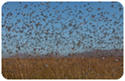
\includegraphics[keepaspectratio]{organisms-that-move/data-image/insect-outbreak.png}}
\pandocbounded{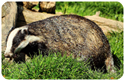
\includegraphics[keepaspectratio]{organisms-that-move/data-image/badger-badger-badger.png}}\end{minipage}%

\caption{\label{fig-animals-we-might-count}Three examples of animals
that might need to be counted, for conservation (e.g.~the Monarch
butterfly, left); for pest control (e.g.~an insect outbreak, centre);
and to predict outbreaks (e.g.~Tb in badgers, right).}

\end{figure}%

There are many areas of ecology and management that rely on estimates of
population size. This might be in a conservation context, wanting to
understand how large your breeding population is and the range that it
covers. It could also be to understand rates of and routes used for
migration, from monarch butterflies to humpback whales.

Understanding population size and spread is important for monitoring
pest control in agricultural and forestry contexts, for example to be
able to predict or minimise the impacts of locust swarms or armyworm
outbreaks in Africa. Insects are not the only pests we might want to
count: we might be looking to reduce numbers of feral cats and rats in
the antipodes in Australia or New Zealand, or wanting to control numbers
of escaped mink in East Anglia.

When looking at controlling populations, it is important that we
understand the population biology of the organism, for example its
reproductive strategies, so that we know how to target the organism and
control it effectively.

We might also want to look at change through time, for example how
populations respond to climate change, whether numbers decline or home
ranges shift. This might be looking at scenarios from the changing
elevation of dung beetles or butterflies, to the feeding range of polar
bears. Similarly, we might want to count animals to monitor disease
outbreaks and predict future spread, and we've seen this over recent
decades with bird flu and swine flu, as well as the perennial debate
about culling badger populations (in the UK) or brushtail possums (in
NZ) and its efficacy in controlling bovine tuberculosis in cattle.

\section{How do we go about estimating population
size?}\label{how-do-we-go-about-estimating-population-size}

We can use counts to monitor population density associated with specific
places in space and time.

When doing this we need to know which individual we are counting,
especially as we can't always see all of the animal population by virtue
of the fact that they are moving. If we can't see animals themselves, we
can use a proxy (Figure~\ref{fig-proxy}). This involves monitoring
calls, tracks, sightings or other evidence like faecal samples, usually
along transects or in fixed monitoring locations as with our plant
monitoring techniques.

We might go to these locations or walk the transects on multiple
occasions to record evidence. We might also use a continuous monitoring
strategy to get an idea of how many individuals are using that location,
for example using camera traps to photograph tigers and then identifying
them by their coat patterns.

\begin{figure}

\begin{minipage}{0.33\linewidth}

\pandocbounded{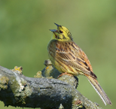
\includegraphics[keepaspectratio]{organisms-that-move/data-image/yellowhammer.png}}

\subcaption{\label{}yellowhammer}
\end{minipage}%
%
\begin{minipage}{0.33\linewidth}

\pandocbounded{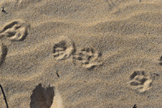
\includegraphics[keepaspectratio]{organisms-that-move/data-image/animal-footprint.png}}

\subcaption{\label{}insect-outbreak}
\end{minipage}%
%
\begin{minipage}{0.33\linewidth}

\pandocbounded{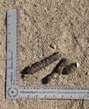
\includegraphics[keepaspectratio]{organisms-that-move/data-image/faecal-sample.png}}

\subcaption{\label{}badger}
\end{minipage}%

\caption{\label{fig-proxy}From left to right: A yellowhammer singing on
a branch; A close up of an animal foot print in the sand; A ruler
indicating the size of a faecal sample on the ground.}

\end{figure}%

The sampling efficiency of this type of methodology is difficult to
estimate. When designing our sampling regimes, we need to consider how
the biology of the species affects the scale of our sampling effort. As
we discussed last week, getting the spatial scale right with respect to
the organism we are measuring is key - just as we wouldn't use a metre
square quadrat to record rainforest trees, or a hectare to count
daisies, we need to consider the home range size and activity of the
animal so that we don't look for wolves for just two days in a small
patch of land when they might be roaming across the landscape and only
visit that part of their territory rarely.

When designing an experiment, think about what properties of the animal
population could impact on the probability of the animal being sampled,
to help you decide whether transects or plots are most appropriate for
recording presence or abundance of the animal, and how the timing of
your data collection should work. Factors to consider include:

\begin{itemize}
\tightlist
\item
  The extent to which the animal roams, on daily, seasonal and annual
  timescales.
\item
  When the animal is active, e.g.~in the day and night, or across the
  seasons
\item
  What behavioural changes might occur during the breeding season, for
  example if birds are incubating eggs, or if there is any kind of
  mating display.
\end{itemize}

If you go out into the field to sample an animal at fixed locations but
don't have any information about territoriality in the species that
you're sampling, then where you place your sampling plots may be
extremely biased and you may not be getting a good estimate of
population size. This would impact on the probability of the animal
being sampled. Similarly, if you're on a track that the animals use
frequently then you may be resampling the same individual all the time,
so there are two components to this challenge of sampling animals. First
of all, we need to determine whether the animal is there at all, and if
so, whether you are sampling different individual animals each time.
Both of these are much more difficult to account for than when we are
studying sessile plants and animals that don't move around.

\section{The Lincoln-Petersen Index}\label{the-lincoln-petersen-index}

There are multiple indices for estimating population size. In this
chapter, we are focusing on the Lincoln-Petersen index.

You may come across a number of names for this index, such as the
Petersen index, the Lincoln index, the Petersen-Lincoln index or the
Lincoln-Petersen index -- this is because this model was derived
independently by both authors in different contexts. Petersen studied
fish, specifically European plaice in the 1890's and Lincoln studied
banding returns in waterfowl in the 1930s. In these notes we may use L-P
index for short but in your own scientific writing (especially for
assessments) please write it out in full.

The L-P index is based on a simple and intuitive model
(Figure~\ref{fig-capture-release}):

\begin{enumerate}
\def\labelenumi{\arabic{enumi}.}
\tightlist
\item
  First we capture \emph{r} individuals.
\item
  We mark all of them and then let them go.
\item
  After an appropriate period of time we have a second capture round,
  collecting \emph{n} individuals.
\item
  We count all \emph{m} individuals in that capture that already have a
  mark.
\end{enumerate}

\begin{figure}

\centering{

\pandocbounded{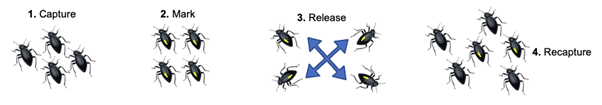
\includegraphics[keepaspectratio]{organisms-that-move/data-image/mark-capture-release.png}}

}

\caption{\label{fig-capture-release}On the first visit, \emph{r} = 4
individuals are captured and marked, from an unknown population size N.
On the second visit a further sample of size \emph{n} = 6 is captured,
of which \emph{m} = 2 individuals are already marked.}

\end{figure}%

The key assumption of the L-P index model is that the *proportion of
marked individuals remains constant** between the first and the second
capture, and so we can estimate population size from the number of
marked individuals that are recaptured as:

\[
{m \over n} = {r \over \hat{N}}
\] or \[
 \hat{N} = {rn \over m}
\]

Where \(\hat{N}\) means an estimate of true population size \emph{N}.

That is, the proportion of marks in the second capture is equal to the
proportion of the whole population that was marked in the first capture.

There is a modification to this equation for small sample sizes, called
the Bailey modification:

\[
\hat{N} = {r(n+1) \over (m+1)}
\]

This can be used in cases where the recapture size is very low,
e.g.~less than 10. You might not use the Bailey modification, but it is
shown here to make you aware that there are adjustments that you can use
to make your estimates of population size more accurate.

\section{Assumptions of the Lincoln-Petersen
index}\label{assumptions-of-the-lincoln-petersen-index}

The Lincoln Petersen model, whilst being a relatively simple model in
form, has a lot of assumptions.

\subsection{Marks are permanent and recorded
correctly}\label{marks-are-permanent-and-recorded-correctly}

The first is that the marks are permanent and correctly recorded:
collars remain on necks and rings on birds don't fall off. For correct
recording this might mean you know that the yellow coloured rings you
fitted on your bird population at the start of a study haven't faded to
white in the last 5 years that you've been monitoring the bird.

\subsection{Marking has no effect on likelihood of
recapture}\label{marking-has-no-effect-on-likelihood-of-recapture}

The index assumes that marking has no effect on the likelihood of
recapture. This is a very interesting and important assumption as there
are certain behaviours that can go along with being marked in animal
populations. Unlike cutting a leaf off a plant which won't necessarily
change its behaviour, and won't change its population size, certain
types of marks are known to have an effect on the behaviour of an
animal.

You can have behaviours that are loosely called trap-happy and trap-shy
behaviour. For example, if you put food traps out in a field for
rodents, say, if you load those up with a good food source then the
animals will learn that it's there and you're more likely to capture an
animal that has been captured before because it knows the trap is there.

Similarly, the experience of being trapped may be sufficiently traumatic
that an animal knows to avoid that area in future, so there are elements
to the act of trapping animals that may change the likelihood of them
being trapped again in the future which will then have an effect on your
sample size.

\subsection{Marking has no effect on death or
emigration}\label{marking-has-no-effect-on-death-or-emigration}

We also assume that marking has no effect on mortality rates or
emigration. If the collar that you put on an animal is so heavy that it
loses mobility and is more likely to be predated then these marked
individuals are disproportionately lost from the population. So, this
impacts on the numbers of marked individuals you find in the second
capture and so impacts the proportion of marks in the initial and final
sample.

There is good evidence that flipper banding in penguins has a
significant effect on fitness and mortality. This has been a commonly
used technique to tag penguins in Antarctica but we now know that it
impacts on banded individuals. Because of this we are now working on
phasing these bands out because it has a marked effect on the population
and using bands to get an estimate of population size is clearly not
viable in this case. Also, we need to be sure that the mark doesn't
impact on emigrating, so marked and unmarked individuals are equally
transient.

\subsection{All individuals have an inherently equal chance of being
caught, or of
dying}\label{all-individuals-have-an-inherently-equal-chance-of-being-caught-or-of-dying}

These assumptions all combine with the effect that all individuals have
an equal chance of being caught and all have an equal chance of survival
from one capture to the next, so the mark has no effect on this.

Anything that happens in the population that means that marked organisms
are more or less likely to be captured will affect your estimates of
population size.

\section{Populations are dynamic}\label{populations-are-dynamic}

Demographic properties of populations are another thing we have to
consider in taking population estimates.

One of the key factors with this model and its assumptions is that we're
looking at a closed population.

We said that an unequal chance of survival due to marking can influence
population estimates. The other thing that can affect the proportion of
marks in the model is that there is recruitment into the population,
either through immigration into it or through birth. Immigrants into the
population and new-borns are inherently unmarked and so this depresses
the proportion of marked individuals in the population so we can think
about what this would then do to our estimates of population size.

This is a significant limitation of the model because it restricts when
you can undertake these mark-recapture sampling efforts based on the
demographics of the species in question. So, you do again have to
understand the biology of the organism that you are sampling.

Most derivations of the L-P model have been developed to model
population change between mark and recapture events. With the simplest
model, Lincoln-Petersen index, there is no demographic change between
the first and the second event. Because of this we need to think about
what is an appropriate measure of time between the first and the second
sampling event for each population. This is akin to considering the
appropriateness of quadrat size when sampling plants and whether you're
looking at daisies or palm trees. In this case we want to get the
sampling time frame right whether we are sampling snails or deer.

\chapter{Building on limitations of the Lincoln-Petersen
index}\label{sec-limitations-lincoln-petersen}

In this section, we'll build on our understanding of the Lincoln
Petersen index, to:

\begin{enumerate}
\def\labelenumi{\arabic{enumi}.}
\tightlist
\item
  Understand the assumptions and therefore limitations of the
  Lincoln-Petersen index
\item
  Appreciate how derivations of the model look to overcome some of these
  limitations
\item
  Understand the importance of timing in models estimating population
  size
\end{enumerate}

\section{Closed populations}\label{closed-populations}

A key assumption we make when using the L-P index to estimate population
size is that the population is closed. A closed population is one in
which there is no immigration or emigration.

Do we ever see closed populations in the wild? We can see closed
populations due to geography, for example when a population becomes
isolated from others and there is no migration between populations.
Metapopulations with very low exchange between populations may be
effectively acting as closed.

The timescale of examination can also result in a (near) closed
population. We must think about the appropriateness of the length of
time between our sampling events. If we look at short intervals, this
may mask long term change for the purposes of analysis; if your research
question is not interested in long term change that might be alright.
Unless you repeat sampling efforts at another time, you won't see any
population change through time. However, if you repeat-sample too
quickly, you will record a snap shot of population size ``in this
location'' as there won't be time for any individuals to move in or out
from the wider area of interest.

\section{Open populations}\label{open-populations}

Open populations are subject to demographic change: immigration,
emigration, birth and death. Here we explore how to incorporate
demographic change in derivations of the L-P index to be more realistic
in estimates of population size. To do this, indices may consider the
loss rate of ``marks'' in subsequent captures or estimate rates of
movement in and out of populations.

\section{The Jolly Seber estimate}\label{the-jolly-seber-estimate}

The Jolly Seber estimate is a derivation of the L-P index that aims to
improve it using repeated sampling, with unique marks for each sampling
time point.

If the population is completely closed, in the way that we assume for
the L-P index, then all of the marked individuals are at risk of being
recaptured. But in a typical population there is a mortality risk and
there is an emigration rate. The repeated sampling in the Jolly Seber
index allows you to assign a probability to recapturing particular
marks. The total number of marked individuals at risk of being
recaptured is central to this method. We can estimate how this is
changing from the number of old marks from previous sampling efforts
that we then recapture.

Figure~\ref{fig-snails-capture-mark} illustrates how repeated sampling
with unique marks could work for a population of snails. After n
sampling sessions, individuals may have 0-n marks, depending on how many
times they have been captured. On each of the capture days, rather than
just recording mark or no mark, as with the L-P index, you would count
how many individuals have no marks, or any combination of the unique
marks that have been applied over the course of the experiment. The
counts of how many individuals you see at each of the time points and
how many marks these individuals have can be used to estimate the total
population size, and also estimate immigration rates and survival rates.

\begin{figure}

\centering{

\pandocbounded{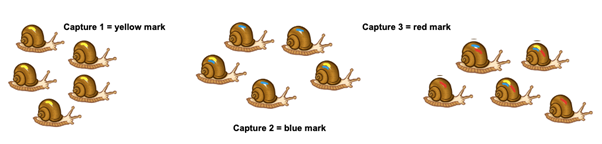
\includegraphics[keepaspectratio]{organisms-that-move/data-image/snails-capture-mark.png}}

}

\caption{\label{fig-snails-capture-mark}On the first capture (left), 5
individuals are captured and marked with a yellow mark, from an unknown
population size N. On the second capture (centre), a further 5
individuals are marked with a blue mark. Two of these also had a yellow
mark, and three are new to being marked. On the third capture (right), 5
individuals are marked with a red mark. Two of these already had a
yellow mark and a red mark, and one had a red mark but no yellow mark.
Two are new to being marked.}

\end{figure}%

You don't need to be able to calculate Jolly Seber estimates yourself in
this module, but you might be interested in reading about it if you are
considering repeat population sampling in the future.

The assumptions of the Jolly Seber index are the same as the L-P index
with regards to marks being permanent and readable and that the marks
won't impact mortality risk. However, as you are undertaking repeated
sampling you can estimate movement into and out of the population
(through mortality or physical movement), and this rate can vary at
different times, giving a very flexible approach to population size
estimation. This model is calculated based on probability distributions
and is just one of the different derivations of the Lincoln Petersen
index.

The original paper by Jolly was performed using black-kneed capsid bugs
over 13 sampling occasions (Figure~\ref{fig-jolly-mark-recapture}). At
each capture, it was recorded when each individual was last captured;
for example, on the seventh capture, 250 bugs were captured, of whom 56
were most recently seen at capture six, 34 at capture five, 10 at
capture four, 5 at capture three, 6 at capture two, and 1 at capture
one: 112 bugs have some combination of marks, and 138 are unmarked.

Reading down the columns provides the number of bugs that were marked on
a given day and subsequently captured again, for example, 101 bugs were
marked on day 6 and turned up in later sampling efforts.

\begin{figure}

\centering{

\pandocbounded{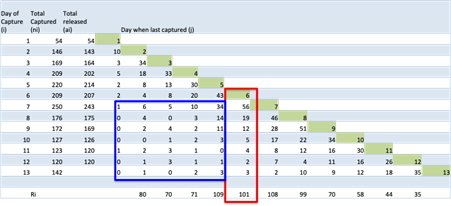
\includegraphics[keepaspectratio]{organisms-that-move/data-image/jolly-mark-recapture.png}}

}

\caption{\label{fig-jolly-mark-recapture}The original mark-recapture
data from Jolly (1965) where the most recent previous marks on each of
the individuals has been recorded over 13 catches. Note that the total
released is increasingly lower than the number captured as there is a
mortality risk associated with capture. For example, of the 146
individuals captured on day 2, only 143 were released.}

\end{figure}%

This method hinges on knowing how many marks there are in the population
at any time point. This isn't an estimate you need to know how to
calculate yourself but you can see the types of estimates you could
calculate from the data collected in this index:

\begin{itemize}
\tightlist
\item
  The number of marks ``at risk'' at day \emph{i} as a function the
  total individuals marked, with a correction for the rate of loss of
  previous marks.
\item
  The population size at day \emph{i}, using the L-P for the subset of
  data from that day and the previous one.
\item
  The survival rate from day \emph{i} to day \emph{i} +1 and the number
  of additions to the population from day \emph{i} to day \emph{i} +1,
  using declines in the proportion of marks over time.
\item
  The standard errors surrounding these estimates.
\end{itemize}

Begon (1983) published a critique of these types of models in Oikos
40:1555 (practice your literature searching skills if you would like to
read the original). It was an interesting reflection on experimental
design and data analysis. His key conclusion was that most studies did
not test whether the assumptions of the models they used were met.
Ultimately not enough studies tested or knew enough about the biology of
a population to see if the immigration, emigration and mortality
assumptions were actually followed.

If you were looking into using these indices in a project setting you
would want to think about being explicit about the assumptions of the
model. You would want to think about being able to justify the
assumptions either in reference to the biology of the organisms you are
testing and consider if you could also test any of these assumptions and
how.

\section{The issue of timing}\label{the-issue-of-timing}

With both the L-P, Jolly Seber and other models that estimate population
size, timing is very important. As we said in sampling plants that the
size of the quadrat needs to be appropriate for the biology of the plant
you are studying. Similarly the timing of sampling efforts is important
for estimating population sizes of animals.

Most sampling methods treat the sampling period when the marks are made
as a single point in time. Mathematically they are instantaneous but in
reality, they are not. Repeated captures are used to some extent to
overcome this, but the time period for the mark-recapture needs to be
short relative to the time interval between the next mark-recapture
effort. For example you may leave some pitfall traps out for 7 days
(this is your sampling period - a week long, rather than a single point
in time) but you probably wouldn't come back and repeat the trapping
within the next week because it would effectively be extending your
sampling period rather than being a `new' time period. Instead you might
wait a month before putting your traps out again.

\section{References}\label{references}

Begon, M. (1983). Abuses of Mathematical Techniques in Ecology:
Applications of Jolly's Capture-Recapture Method. Oikos, 40(1),
155--158. https://doi.org/10.2307/3544213

\chapter{Methods for sampling animal
populations}\label{sec-methods-sampling-animal-populations}

Here we will explore some of the methods we can use to sample animal
populations, in order to gather data with which to estimate population
sizes and learn about individuals and populations in a location. We will
focus on sampling invertebrates and larger vertebrates. You should: -
Appreciate the varied methods used to accurately sample animal
populations - Understand how the methods used should be appropriate to
the life history of the animal and be able to consider the strengths and
limitations of sampling methods.

\section{Day flying invertebrates}\label{day-flying-invertebrates}

It's one thing to count individuals and model population sizes, but
first we have to collect the data with which to do the analyses. When
you choose a sampling technique, once again you need to use a method
appropriate to the biology of the organism that you're studying. For
example, you wouldn't use a fishing net to catch snails!

Day flying insects can be caught using a variety of methods: - sticky
traps - malaise traps - water traps - nets

Malaise traps (Figure~\ref{fig-malaise-traps}) are adapted to the
biology of the organism they're looking to catch. Flying insects will
look to go up and over any barriers they encounter, as they are not
burrowing organisms. So, if you see an insect trapped in a house it will
fly upwards at the window. This behaviour is what the malaise trap
exploits.

It is a type of tent with open sides and a net barrier down the middle.
The insects fly into the barrier in the middle and to try and get away
from this barrier they go up. They continue moving up the sloped roof of
the tent and at the highest point of the roof there is a gap that the
insect crawls through. This gap leads to a bottle with ethanol or
another preservative in it. Given that this trap exploits a typical
behaviour of day flying insects it is a very effective way to take an
estimate of what is flying around in an area at a particular time.

\begin{figure}

\centering{

\pandocbounded{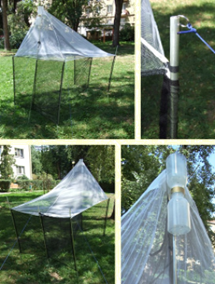
\includegraphics[keepaspectratio]{organisms-that-move/data-image/malaise-traps.png}}

}

\caption{\label{fig-malaise-traps}Malaise traps, showing the tent like
structure and preservative bottles at the apex.}

\end{figure}%

Water traps (Figure~\ref{fig-water-and-sticky-traps}) have a flat sheet
of some sort that the insects can't grip onto. This sheet is in a colour
that the insect is attracted to, for example pollen beetles are
attracted to the colour yellow, so you have a yellow Perspex plate, the
insects fly towards it, try to land on it but they can't grip and so
they slide down. The Perspex sheet sits in a tub of water that the
insect lands in after sliding down, which it can't then escape from.

You will see examples of Sticky traps in the glasshouses around the
department (Figure~\ref{fig-water-and-sticky-traps}) and these can be
baited with insect pheromones or other baits appropriate to your target
organism. The insect flies towards it and can't escape.

\begin{figure}

\begin{minipage}{0.50\linewidth}
\pandocbounded{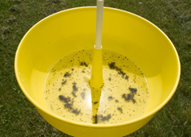
\includegraphics[keepaspectratio]{organisms-that-move/data-image/water-trap.png}}\end{minipage}%
%
\begin{minipage}{0.50\linewidth}
\pandocbounded{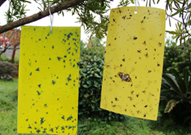
\includegraphics[keepaspectratio]{organisms-that-move/data-image/stick-trap.png}}\end{minipage}%

\caption{\label{fig-water-and-sticky-traps}Water traps (left) and sticky
traps (right).}

\end{figure}%

You have probably seen a butterfly net before; these are useful for day
flying insects.

\section{Night flying invertebrates}\label{night-flying-invertebrates}

For night flying insects you can use light to attract individuals.
Figure~\ref{fig-robinson-trap} shows a Robinson trap, which uses a
mercury vapour bulb to attract moths. Skinner traps work similarly but
are more of a box shape. Moths are attracted to the light, but when they
collide with the Perspex cross barrier in the middle, they fall down
into the box. This is full of cardboard and places for the moths to rest
until daytime. You can then count them whilst they are at rest and then
let them go so it is a non-destructive sampling technique.

\begin{figure}

\begin{minipage}{0.50\linewidth}
\pandocbounded{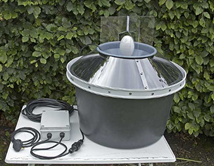
\includegraphics[keepaspectratio]{organisms-that-move/data-image/external-robinson-trap.png}}\end{minipage}%
%
\begin{minipage}{0.50\linewidth}
\pandocbounded{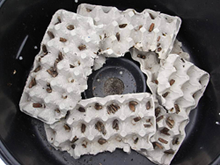
\includegraphics[keepaspectratio]{organisms-that-move/data-image/internal-robinson-trap.png}}\end{minipage}%

\caption{\label{fig-robinson-trap}A Robinson trap showing the external
set up (left) and the hiding places inside (right).}

\end{figure}%

\section{Non-flying insects}\label{non-flying-insects}

Not all insects fly so we also need to think about how to capture
non-flying insects and other invertebrates. Methods include: - Pitfall
traps, in which insects fall into a trap dug into the ground (you will
have an opportunity to do this later in the semester); - Sweep nets,
which are used to sweep across vegetation and catch vegetation; - D-vacs
are similar to a hoover, and you can hoover up a whole community of
insects sitting on a plant's leaves; - Tree beating, in which you
collect insects on a sheet after devising a sampling method that
involves hitting the tree at a certain height for a specific number of
repetitions.

The key thing you can take from all of these different methods is that
if you went to a site and said I want to enumerate the entire
invertebrate or insect community from this site, it would be very
difficult to do that by relying on just one method. You will need
different sampling methodologies to capture different functional groups
of insects.

\section{Pitfall traps and beetles}\label{pitfall-traps-and-beetles}

For pitfall traps, you take a core out of the soil and use a cup
containing different liquids to capture different functional groups.
Some may be water; some may be washing up liquid or antifreeze. We need
to consider the content as some groups may be attracted to different
types of compounds.

Pitfall traps are particularly good for animals that move quickly over
the soil surface. If you're using them to look at multiple species in a
community, the abundance of each of the different types of organism and
the density that you calculate is a function of how quickly that
organism moves.

If an organism is slow and it has a small range, you'll see fewer of
them across your pitfall traps than an organism that moves around very
quickly and this impacts on the probability of them being captured. The
faster they move, the more likely they are to walk into one of your
pitfall traps, the slower they move, the less likely they are to
encounter a pitfall trap.

\section{Pitfall case study}\label{pitfall-case-study}

Garcia \emph{et al.} (2000) looked at a ground dwelling beetle,
\emph{Nebria brevicollis}, which is an aphid-eating woodland species.
They studied it in a field margin, using repeated sampling to calculate
the activity density (as a proxy for population density) of the beetles
at different distances from the hedge
(Figure~\ref{fig-brevicollis-hedge}). They acknowledge that the number
of individuals they catch is a function of how busy they are, as well as
how densely they occur.

\begin{figure}

\centering{

\pandocbounded{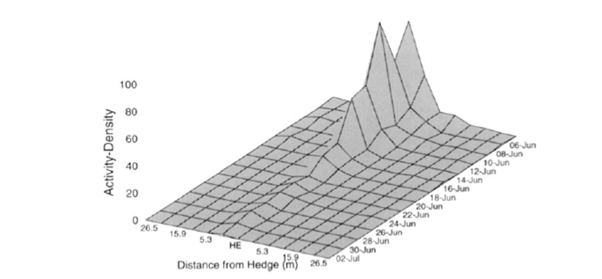
\includegraphics[keepaspectratio]{organisms-that-move/data-image/brevicollis-hedge-distance.png}}

}

\caption{\label{fig-brevicollis-hedge}Time series of total activity
density (vertical up the page) of \emph{N. brevicolllis} against date
(y-axis, with time running from the 'back; of the page towards the
front) during aestivation in the field boundary. Activity-density summed
down columns of traps parallel to hedgerow (HE) in cross-section across
the experimental site (x-axis, left to right on the page), through the
hedgerow. Reproduced from Fig. 1 of Garcia \emph{et al.} (2000).}

\end{figure}%

\section{Sampling larger animals}\label{sampling-larger-animals}

When sampling larger animals we can use a wide variety of methods
depending on the biology of the animal of interest: - By trapping and
marking: Longworth traps, mist netting, collaring etc. - By observing:
Camera traps can ID animals with unique markings, e.g.~tigers and other
big cats - By hearing: Bird and other calls have been used, but harder
to identify recaptures. Used to estimate population density

Mist nets are used for birds and bats; they can be banded or marked and
then released. You can also trap and mark animals, for example using
Longworth traps (Figure~\ref{fig-trapping-methods}). These are humane
traps for rodents up to the size of a squirrel. You bait the box at the
end and the animal triggers a trap door as it goes in. You go back in
the morning, count and mark the individuals and then release them.

We can also sample larger animals by observing them. This might include
using camera traps to ID animals that have unique markings such as
tigers and other big cats. We can also identify zebras and giraffes
using this methodology.

In dense habitats it can be useful to use bird calls and other noises to
track animals. You can estimate population density and behaviour with
these methods as animals may be making calls in a territorial or mating
context for example. With these methods it can be difficult to identify
recaptures though as you can't necessarily tag a call to a certain
individual.

\begin{figure}

\begin{minipage}{0.50\linewidth}
\pandocbounded{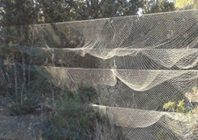
\includegraphics[keepaspectratio]{organisms-that-move/data-image/mist-nets.png}}\end{minipage}%
%
\begin{minipage}{0.50\linewidth}
\pandocbounded{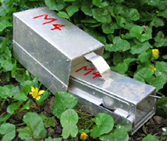
\includegraphics[keepaspectratio]{organisms-that-move/data-image/longworth-traps.png}}\end{minipage}%
\newline
\begin{minipage}{0.50\linewidth}
\pandocbounded{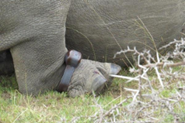
\includegraphics[keepaspectratio]{organisms-that-move/data-image/id-gps-tags.png}}\end{minipage}%
%
\begin{minipage}{0.50\linewidth}
\pandocbounded{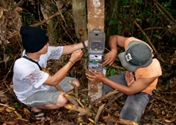
\includegraphics[keepaspectratio]{organisms-that-move/data-image/motion-sensor-cameras.png}}\end{minipage}%

\caption{\label{fig-trapping-methods}Methods for sampling larger animals
(clockwise from top left): Mist nets, Longworth traps, motion sensor
cameras and ID tags with GPS.}

\end{figure}%

\section{Case study: frog calls and
recapture}\label{case-study-frog-calls-and-recapture}

Nelson and Graves (2004) used amateur recorders to log the calls of
\emph{Rana clamitans}, and correlated the call records with a mark
recapture experiment as a way to measure abundance. They were able to
show that there was a relationship between the number of calls and frog
density, but that it was a non-linear relationship
(Figure~\ref{fig-frog-calls}).

\begin{figure}

\begin{minipage}{0.50\linewidth}
\pandocbounded{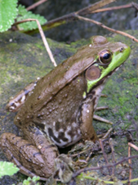
\includegraphics[keepaspectratio]{organisms-that-move/data-image/frog.png}}\end{minipage}%
%
\begin{minipage}{0.50\linewidth}
\pandocbounded{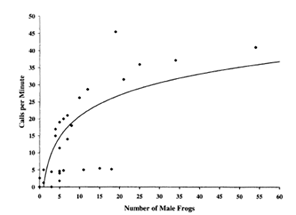
\includegraphics[keepaspectratio]{organisms-that-move/data-image/male-frog-calls.png}}\end{minipage}%

\caption{\label{fig-frog-calls}Male frog (\emph{Rana clamitans}, left
panel) calls per minute (y axis, right panel) increase with number of
male frogs (x axis). Individual data points are shown for each frog,
clustering under 15 frogs and 30 calls per minute. The trend follows an
upwards curve that plateaus at approximately 60 frogs and 35 calls per
minute.}

\end{figure}%

As the number of male frogs increases, the number of calls plateaus: the
male frogs call more when the population is not as dense and we can see
that there is a behavioural element to the amount of calling the males
do. There is another bias to these population estimates as only the
males make these calls: it is a territorial call that the males make
prior to mating. The females were unsurprisingly underestimated in this
study and so this is another clear example of the biology of an organism
impacting on the data that you get, in relation to the sampling methods
you use.

\section{Examples of marks}\label{examples-of-marks}

Other examples of some of the marks you might use to identify
individuals and count abundance include a number of types of clipping
and marking.

To produce unique identifying marks in birds we can clip nails. In the
past, toe clips have been used in frogs. These create unique identifying
combinations. However, we do need to be sure that these methods meet
with current ethical standards and approvals.

Wing clipping in butterflies has previously been common but as with the
assumptions of the mark recapture models you would have to be sure that
it wouldn't affect their ability to fly.

Pen and paint marking on beetle wings or ants and unique shapes of hair
clipping in small mammals are other methods used. These fur clips in
fixed locations on the body can be a way of marking small mammals
without needing tags or collars.

\section{Camera trapping}\label{camera-trapping}

Camera trapping is a non-invasive methodology used to identify unique
individuals, and was first formalised as a methodology by Karanth and
Nicholls (1998). They set out to estimate the population size of tigers
in India (Figure~\ref{fig-tiger}). Camera trapping was used as an
alternative to estimating using footprints, as previously the density of
the individuals had been estimated using the number and the freshness of
the footprints on the trails that tigers regularly use trails to mark
out their territories.

Camera trapping could exploit these trails to identify which individuals
were using them and estimate population size. Using cameras is now an
established technique with methodologies that take into account things
like the density of the cameras.

\begin{figure}

\centering{

\pandocbounded{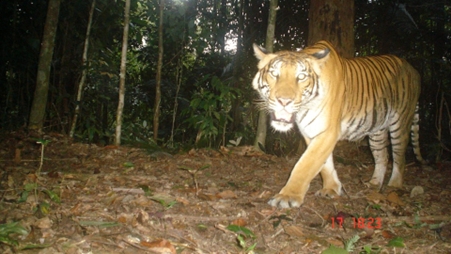
\includegraphics[keepaspectratio]{organisms-that-move/data-image/tiger.png}}

}

\caption{\label{fig-tiger}A tiger walking in the woods, caught on
camera.}

\end{figure}%

\section{Tracking tunnels}\label{tracking-tunnels}

Another non-invasive method for estimating indices of population density
is tracking tunnels. Figure~\ref{fig-tracking-tunnels} shows a simple
mock-up of a tunnel with bait in the middle. Pieces of paper are clipped
to the tunnel on either side of the bait. There is tape on either side
of the bait which has a non-toxic neutral coloured paint mixed with
vegetable oil painted over it, so to get at the bait the animal has to
walk through the paint and they then leave footprints behind after
traversing the paper having reached the bait (Figure~\ref{fig-prints}).

\begin{figure}

\begin{minipage}{0.50\linewidth}
\pandocbounded{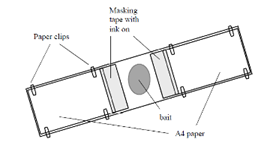
\includegraphics[keepaspectratio]{organisms-that-move/data-image/tracking-tunnels-diagram.png}}\end{minipage}%
%
\begin{minipage}{0.50\linewidth}
\pandocbounded{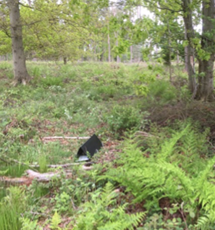
\includegraphics[keepaspectratio]{organisms-that-move/data-image/tracking-tunnel-live.png}}\end{minipage}%

\caption{\label{fig-tracking-tunnels}Tracking tunnels (left) usually
have bait in the centre, and animals have to walk over an ink pad to
reach it. On their way out, they leave footprints on the paper, and can
be identified to species level. We will use tracking tunnels later in
the semester to see what is active on campus, and the photo on the right
shows a tracking tunnel in action on the North York Moors, during a
field trip to Ellerburn in 2015.}

\end{figure}%

\begin{figure}

\begin{minipage}{0.33\linewidth}
\pandocbounded{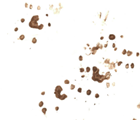
\includegraphics[keepaspectratio]{organisms-that-move/data-image/hedgehog-prints.png}}\end{minipage}%
%
\begin{minipage}{0.33\linewidth}
\pandocbounded{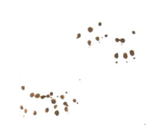
\includegraphics[keepaspectratio]{organisms-that-move/data-image/rat-prints.png}}\end{minipage}%

\caption{\label{fig-prints}\pandocbounded{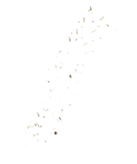
\includegraphics[keepaspectratio]{organisms-that-move/data-image/beetle-prints.png}}
Footprints left in tracking tunnels by a hedgehog (left), rat (centre)
and burying beetle (right).}

\end{figure}%

You can influence what goes through the tunnels depending on the type of
bait that you put out -- this might be rats, beetles or hedgehogs.

\section{Case study: tracking
tunnels}\label{case-study-tracking-tunnels}

Tracking tunnels have been used to monitor animals like brushtail
possums (\emph{Trichosurus vulpecula}) to detect their prevalence in
different habitats and also to detect threatened insects like giant wētā
in New Zealand (Figure~\ref{fig-giant-weta}). In these cases, the number
of footprints is an estimate of density.

\begin{figure}

\begin{minipage}{0.50\linewidth}
\pandocbounded{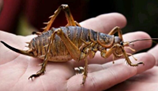
\includegraphics[keepaspectratio]{organisms-that-move/data-image/giant-weta-image.png}}\end{minipage}%
%
\begin{minipage}{0.50\linewidth}
\pandocbounded{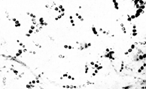
\includegraphics[keepaspectratio]{organisms-that-move/data-image/giant-weta-footprints.png}}\end{minipage}%

\caption{\label{fig-giant-weta}Giant wētā (left) and their footprints
(right) caught in tracking tunnels in New Zealand (Watts et al.~2008).}

\end{figure}%

\section{Animal sampling ethics and
welfare}\label{animal-sampling-ethics-and-welfare}

When sampling any animal population, we have to think about the sampling
technique and if it is destructive or not. This has conservation
implications for example. If you are live trapping and releasing animals
you must consider their welfare and to do that you need to understand
the biology of the organism and the logistics of the sampling process.

For example, Longworth trapping needs a license for mammal trapping in
the UK and there are only certain times of the year when you're allowed
to set up traps like this so that you're not trapping animals during the
breeding season. If a mother is caught in a trap during the breeding
season when foraging for young and is caught overnight then the
offspring could die. These regulations are in place to consider this.

For moth traps we still need to think about welfare, for example
monitoring how many moths die of those that you catch. One of the most
problematic things here is keeping moths in a trap for too long. Traps
need clearing daily but we don't want to then release them such that
after release the moths are resting all day and local birds can easily
predate them, so there are considerations for an appropriate release
consideration here.

\section{References}\label{references-1}

Garcia et al.~Ann Appl Bid 2000 137: 89-97

Nelson, G. L., \& Graves, B. M. (2004). Anuran Population Monitoring:
Comparison of the North American Amphibian Monitoring Program's Calling
Index with Mark-Recapture Estimates for Rana clamitans. Journal of
Herpetology, 38(3), 355--359.

Karanth, K. U., \& Nichols, J. D. (1998). Estimation of Tiger Densities
in India Using Photographic Captures and Recaptures. Ecology, 79(8),
2852--2862. https://doi.org/10.2307/176521

Watts, C. H., Thornburrow, D., Green, C. J., \& Agnew, W. R. (2008).
Tracking tunnels: a novel method for detecting a threatened New Zealand
giant weta (Orthoptera: Anostostomatidae). New Zealand Journal of
Ecology, 32(1), 92-97. https://www.jstor.org/stable/24058104

\part{Species Richness}

\{\#sec-species-richness-overview\}

In the last two chapters, we have explored how to sample populations of
things that move (e.g.~animals) and things that don't move (including
plants).

In this chapter, we will start to consider how we can understand
communities, or collections of populations, that are all present in the
same place at the same time. We'll start by exploring how we estimate
how many species (populations) are present, using observational data
(Chapter~\ref{sec-characterising-communities}). This will take us
towards ideas about how some species in a community are more common and
others are rarer, i.e.~the number of individuals, or the size of the
population, of each species differs
(Chapter~\ref{sec-commonness-and-rarity}). We'll then consider how these
community compositions might affect estimates of species richness, and
how to compare between communities with different sampling effort
(Chapter~\ref{sec-measuring-species-richness}). Finally, we'll go over
concepts of randomisation and rarefaction in a case study from a paper
examining censuses of breeding bird populations
(@sec-bird-survey-case-study). And, because there's a lot of concepts in
this chapter, we'll end with a brief summary
(@sec-species-richness-summary) before you move on to the next bit of
content.

In the workshop this week you will apply some of these sampling
techniques to your LEGO community, and (weather dependent) estimate the
species richness of the waterfowl community on the Campus West lake.

\chapter{Characterising
communities}\label{sec-characterising-communities}

\section{Questions we can answer by looking at communities of
populations}\label{questions-we-can-answer-by-looking-at-communities-of-populations}

When we look at a community of organisms through a scientific lens, we
may have a number of different questions that we want to answer.
Generally speaking, these are the what, the where, the who, the how, and
the why. The kind of questions we may ask include: - How are groupings
of species distributed in nature? (the \textbf{what} - what is going
on?) - How are these groupings affected by their abiotic environment?
(the \textbf{where}, but also potentially the why) - How are these
groupings affected by interactions among species? (the \textbf{who} -
who is interacting?)

This all sounds simple: go somewhere, count the species present! But
there are a number of considerations we need to take into account when
designing an experiment to really understand what is present, and
whether a species is really absent or if we just haven't found it yet.

\section{Scales of communities and
environments}\label{scales-of-communities-and-environments}

The scale (in time and space) that we use to ask questions about
communities can vary across a wide range of scales
(Figure~\ref{fig-scales-communities}). If we are interested, for
example, in the limitations of where vegetation spreads, we might look
at a very large scale, considering whole biomes. This might lead us to
conclude that climate (an abiotic factor) is broadly limiting the spread
of various species of trees and plants. In equatorial regions, we'd see
tropical forests, while in the extreme north we might see boreal forest
or tundra, all of which are characterised by different vegetation types.

However, we can also consider communities at smaller scales. For
example, we might be interested in different mountainous regions, and
the environmental and ecological drivers behind different plant and
animal communities in these regions. We could go even smaller, and think
about the pond in your back garden, or all the way down to the gut
microbiome. All of these different scales of environment may have
different whats, wheres, whos, hows, or whys driving the community
composition.

\begin{figure}

\centering{

\pandocbounded{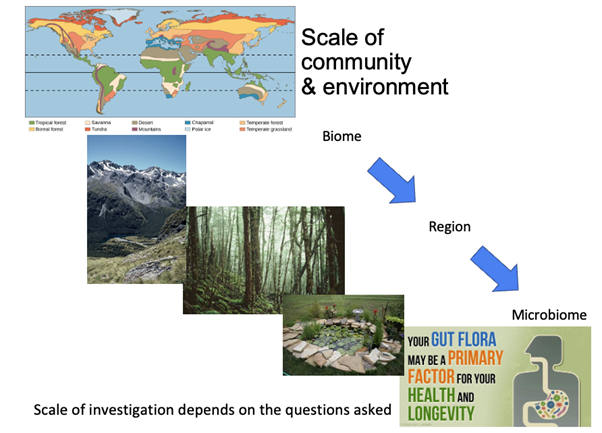
\includegraphics[keepaspectratio]{species-richness/data-image/scales-of-communities.png}}

}

\caption{\label{fig-scales-communities}Scales of different communities
and environments.}

\end{figure}%

\section{What is a species?}\label{what-is-a-species}

Species richness is considered to be the number of species in a given
taxon in the community. But how do you define a species? We generally
use the biological species concept, but any of these potential
approaches may be used: - Biological species - Phylogenetic species -
Cohesion concept - Species discrimination - Morphotypes/morphospecies

The phylogenetic species concept is where a species is the smallest
group of populations that can be distinguished by a unique set of
genetic traits (Figure~\ref{fig-phylogenetic-tree}, with five species
A-E).

The cohesion concept says that a species is a series of populations with
genetic or demographic cohesion, rather than a biological species
(Figure~\ref{fig-phylogenetic-tree}, two species, with small-eared and
big-eared groups).

We may also have the challenge of discriminating between species that
are very similar looking species, or 'cryptic species.'It is not always
easy to tell the difference between them without DNA testing
(Figure~\ref{fig-phylogenetic-tree}, differences between species C, D
and E).

\begin{figure}

\centering{

\pandocbounded{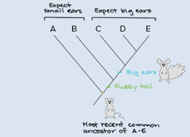
\includegraphics[keepaspectratio]{species-richness/data-image/phylogenetic-tree-example.png}}

}

\caption{\label{fig-phylogenetic-tree}A phylogenetic tree for fictional
small rodent-like creatures with different ears and tails.}

\end{figure}%

This means that, in your community, species richness can go up if you
split up previously lumped species or distinguished cryptic species, or
it can go down where a single species is identified as previously having
two scientific names attached to it. The approach that you choose to
take to identify the species in your community must be carefully
considered as part of your experimental approach when surveying species
richness.

\section{What does species richness tell us about a
community?}\label{what-does-species-richness-tell-us-about-a-community}

``What is present here?'' is one of the first questions an ecologist
might ask about a community. At its heart, this is a question about
species richness: if we sample this location, and we count or collect
individuals of our taxa of interest, what species will those individuals
belong to?

Of course, a community is made up of a variety of species, but it's
unlikely that each species is going to be represented by the same number
of individuals. Some species are more common, with a large number of
individuals, and some are rare, with fewer individuals. This might be
because common species have out-competed the rarer species, or perhaps
because the rarer species have found it harder to survive in this
environment, or have less appropriate habitat. Ultimately, we want to
describe the relationship between the number of species, and the number
of individuals in those species, with respect to the environment and the
biotic interactions that occur, and have occurred, in that location.

As researchers, the question then becomes - what do we measure, in order
to look at the number of species, and these patterns of rarity and
commonness across the set of species that makes up the community? We
could measure the number of individuals in a species, but we could also
measure the total biomass within a community that can be attributed to
each species. Which of these two approaches (or proxies for each one)
that you use will depend on what it is that you are investigating.

\section{What is true species
richness?}\label{what-is-true-species-richness}

When assemblages consist of relatively well-known flora and fauna, and
there are relatively few species, it's possible to record them all and
have a good idea that you've measured all of them. This might be the
case if surveying a temperate zone, and/or a habitat with clear
boundaries, such as a lake or a small island, allowing you to document
it well. There may also be historical records that you can use. Often
this documentation is of assemblages of invertebrates or higher order
plants: things that are easy to define
(Figure~\ref{fig-easily-defined-things}).

\begin{figure}

\centering{

\pandocbounded{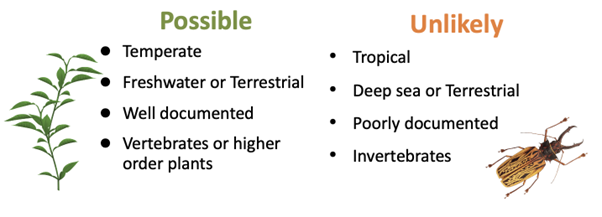
\includegraphics[keepaspectratio]{species-richness/data-image/easy-to-identify-things.png}}

}

\caption{\label{fig-easily-defined-things}Scenarios in which you may be
able to census the species present and record `true' species richness
(left) and scenarios in which it is unlikely that you can find all the
species present, in which case you will only be able to record
`observed' species richness.}

\end{figure}%

You are probably not observing true species richness if you're working
in a tropical zone, because it is incredibly diverse. Similarly, areas
allowing a lot of movement in and out of the habitat, such as a deep sea
area, mean that you may not know if you've recorded all species present.
These locations tend to be poorly documented, and that might be because
of limited funding to look into these habitats. Often they are highly
diverse, and in these areas true species diversity is never going to be
recorded. We have to make do with an estimate. It could also be that
your study species, such as invertebrates, is incredibly diverse with a
lot of cryptic species. This means that, for any measure of species
richness, we need to consider how likely it is that we're going to find
all of the species present, even with a good sampling effort.

\section{Case study: Yasuni rainforest, Ecuadorian
Amazon}\label{case-study-yasuni-rainforest-ecuadorian-amazon}

One approach to recording species richness is to measure the number of
species found in a given area. In the Ecuadorian rainforest of Yasuni in
the Amazon, an experiment was undertaken to assess species richness.
Initially, researchers used a one hectare (100m x 100m) search area,
counting the trees within this area with a measurement of the diameter
at breast height (DBH - i.e.~about 4 feet above the ground) of more than
10 cm. These are considered established trees, as opposed to saplings or
seedlings. The study found seven hundred individual trees, representing
253 species -- clearly a diverse area. The researchers then wanted to
examine whether increasing the search effort increased the number of
species observed.

When the search area was increased to 25 times the size, they found over
17 thousand individual trees, but only four times as many species
(Table~\ref{tbl-amazon-rainforest-species}). The species count did not
increase proportionally to the increased sampling effort, meaning that
we can't simply assume in this region that species richness is a
function of sampling area. This also makes it hard to compare different
regions, as we can't assume a linear relationship between the sampled
area and the species richness.

\begin{longtable}[t]{lllll}

\caption{\label{tbl-amazon-rainforest-species}Individual and species
counts from searching different areas and tree sizes in the Ecuadorian
Amazon rainforest}

\tabularnewline

\\
\toprule
 & Search area & Search critera & Number of trees & Number of species\\
\midrule
 & 1 ha & DBH > 10 cm & 702 & 253\\
 & 25 ha & DBH > 10 cm & 17 550 & 820\\
 & 25 ha & DBH > 1cm & 152 350 & 1140\\
\bottomrule

\end{longtable}

The researchers also asked what would happen if we increased the
available population to sample not just adult trees, but all the way
down to the smallest saplings? Excluding seedlings that have not reached
4 feet tall, but counting all plants that have reached greater than four
feet, regardless of their DBH, the number of trees present that reach
this criteria increased substantially, from over 17 thousand to over 152
thousand. There was also an increase in the number of species counted,
but again disproportionate to the increased sampling effort.

The demographics of the population, and the way that sampling is carried
out, will affect records of observed species richness. We need a way to
calculate `true' species richness if we want to be able to compare
studies that use different sampling regimes, or be resilient to changes
in sampling effort within a single study. This calculation of how many
species there really are in a given area should be independent of
effort, to be comparable between sites.

\chapter{Commonness and rarity matters}\label{sec-commonness-and-rarity}

\section{Patterns of commonness and
rarity}\label{patterns-of-commonness-and-rarity}

A community is made up of a collection of populations of different
species, but it is unlikely that each species is going to be represented
by the same number of individuals. Some species are more common, with a
large number of individuals, and some are rare, with fewer individuals.
This might be because common species have out-competed the rarer
species, or perhaps because the rarer species have found it harder to
survive in this environment, or have less appropriate habitat. To
understand the composition of a community in relation to its history and
its environment, we want to be able to describe the relationship between
the number of species, and the number of individuals in each of those
species.

Whittaker plots (also called rank-abundance plots) are a measure of how
abundance progressively decreases from the most common to the most rare
species in the community. On the y axis, we can plot the abundance or
the relative abundance of each species, and we can plot that against
their rank. We plot the most abundant species close to the origin, then
the next abundant, then the next, all the way to the least abundant
species.

\section{Case study: the grassy bank near the
library}\label{case-study-the-grassy-bank-near-the-library}

In previous years, students on this module have done fieldwork projects
using vegetation surveys on the grassy bank near the library. In this
dataset we have the abundance of various species, ranked them by their
commonness (Figure~\ref{fig-library-abundance}). In total, 49 species of
plant were counted across a number of quadrats. The top 5 species
account for 50\% of the total number of individuals. There is a
relatively large drop in the relative abundance between species 1 and 2
and species 4 and 5, but as the rarity of species increases, we start to
see less of a difference in the relative abundance of individuals.
Comparing the data graphed with a linear y axis
(Figure~\ref{fig-library-abundance}, left) with a log y axis
(Figure~\ref{fig-library-abundance}, right), we can see the relationship
is an exponential decay. With the linear y axis, we get a steep drop in
abundance through the first 5 most common species, followed by a
plateauing of the relative abundance of individuals in the less common
species. On the right, we see a straight line of decreasing relative
abundance. The log scale tells us that increasing in rank in the
community (i.e.~increasing rarity) is associated with a relative
decrease in abundance by an order of magnitude.

\begin{figure}

\centering{

\pandocbounded{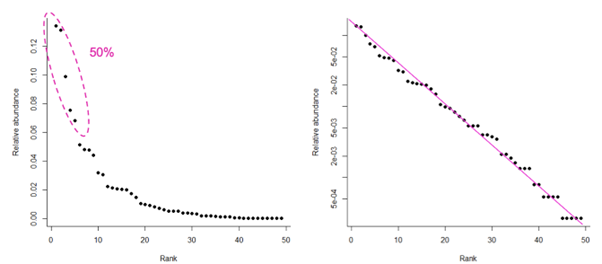
\includegraphics[keepaspectratio]{species-richness/data-image/library-rank-abundance.png}}

}

\caption{\label{fig-library-abundance}Two versions of the rank abundance
plot of 49 plant species found on the grassy bank near the University of
York library. Half of the individuals come from the five most common
species (left, pink dashed ellipse). Note the log scale on the right
panel, which changes the shape of the data to a straight line.}

\end{figure}%

\section{Evenness and dominance}\label{evenness-and-dominance}

In addition to determining which species are the most abundant, rank
abundance plots also help us to work out the \textbf{observed species
richness} of a community. We know how many species have been recorded in
the study in total - that is our highest ranking species, or our rarest
species, on the x axis (Figure~\ref{fig-rank-abundance-plot-guide}).

We can also see how rapidly the abundance decreases from the commonest
to the rarest species in the community. This means we can assess the
\textbf{evenness} of the community: how similar the species are in their
abundance, or how abundant are the very rare species compared to the
most common species (Figure~\ref{fig-rank-abundance-plot-guide}).

Finally, we can see the extent to which one or a few species dominate
the community. The steeper or more curved the line, the more the common
species have a greater degree of \textbf{dominance} in the community
compared to the rarer species
(Figure~\ref{fig-rank-abundance-plot-guide}). A straight line with a
negative slope, however, would imply that there's a fairly consistent
decrease in abundance of individuals as rarity increases, so while the
community is not even, there are fewer species with a high degree of
dominance over others.

\begin{figure}

\centering{

\pandocbounded{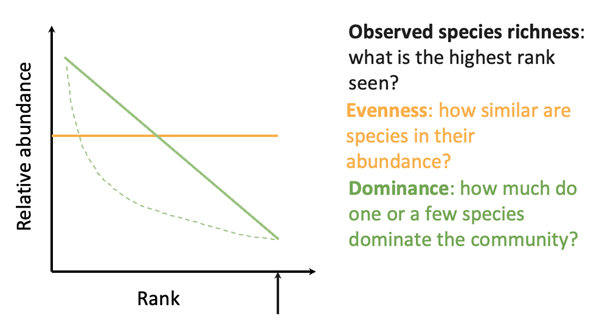
\includegraphics[keepaspectratio]{species-richness/data-image/rank-abundance-example.png}}

}

\caption{\label{fig-rank-abundance-plot-guide}How to read observed
species richness (black arrow), evenness (orange horizontal line) or
dominance (green solid and dashed lines) on a rank abundance plot.
Observed species richness is the highest rank plotted on the graph. A
totally even community has the same number of individuals in each
species. The steeper the slope on the graph, the less even is the
community, with a greater chance that the most common species are
dominant over the rarer species.}

\end{figure}%

\section{Case study: Rank abundance in
forests}\label{case-study-rank-abundance-in-forests}

Plotting the relative abundance of species found in different forests
can help us to understand how the communities differ
(Figure~\ref{fig-rank-abundance-forests}). The rank abundance plot of
the boreal forest shows a straight line: there are very few species in
total, and there is a high degree of dominance of only a few species. As
we move through temperate deciduous and tropical semideciduous forests,
towards the equator, we can see higher species richness appearing (the
lines on the plot are longer, reaching higher ranks). We also see more
evenness; the lines are less steep particularly in the middle ranks of
the community. Finally, in the tropical evergreen forest, there is both
a high degree of species richness (with a very high maximum rank), and a
higher degree of evenness, as the slope of the line is much shallower
than for the boreal forest even when we reach the rarer species.

\begin{figure}

\centering{

\pandocbounded{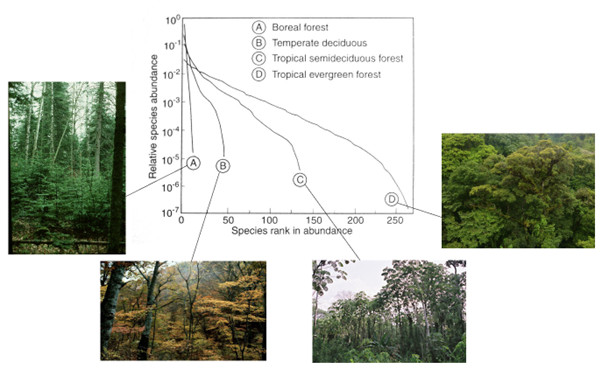
\includegraphics[keepaspectratio]{species-richness/data-image/rank-abundance-forests.png}}

}

\caption{\label{fig-rank-abundance-forests}Rank abundance of species
differs between (A) boreal forest, (B) temperate deciduous forest, (C)
tropical semideciduous forest, and (D) tropical evergreen forest. Note
the logarithmic y-axis scale.}

\end{figure}%

We'll come back to relative abundance of species in more detail next
week.

\chapter{Measuring species
richness}\label{sec-measuring-species-richness}

\section{Cumulative species richness and sampling
effort}\label{cumulative-species-richness-and-sampling-effort}

When we sample a community to estimate species richness, we need to
think about how our sampling effort changes what we can observe. If we
put no effort in, we know that we don't see any species. So how does the
number of species relate to the amount of effort that we put in?

Using your LEGO communities as an example, think about taking a handful
of bricks out of the bag. How many species do you find? Initially you
might discover a lot of new species: for example, a first handful of ten
bricks might give you 7 different shapes or colours of brick. If you
took another handful about the same size, are they all the same
`species' as the initial seven? And, if not, how many new ones have you
found? You are likely to find in your second sample that you find fewer
individuals from as yet unseen species. If you were to keep sampling,
would you find any more species?

The cumulative number of species found can be plotted against increasing
effort, to get the characteristic curve called a species accumulation
curve (Figure~\ref{fig-species-accumulation-curve}). The curve has an
initial steep slope, as the species found at the beginning must be new
to the record. As we take more samples, we start to see the same species
reappearing. New species may continue to turn up, but they're
increasingly less likely. Even though we're putting in more effort, our
cumulative tally slows down. Eventually you may eventually conclude that
you've got a good representation of the community, because the curve is
tending to the horizontal. We can never be certain that we have sampled
enough, and that we are not going to find a new species, but we can be
reasonably sure.

\begin{figure}

\centering{

\pandocbounded{
\includegraphics[keepaspectratio]{species-richness/species-richness-measuring-species-richness_files/figure-pdf/fig-species-accumulation-curve-1.pdf}}

}

\caption{\label{fig-species-accumulation-curve}Species accumulation
curve: initially the species tally increases quickly, but then slows
down with increased sampling effort. New species may continue to turn up
even after a lot of effort has been expended.}

\end{figure}%

\section{Species accumulation curves}\label{species-accumulation-curves}

In order to increase confidence in your estimates, we might sample a
number of different sites across the community and record the number of
species at each one. Combining the results can help us to analyse the
data and make them comparable with other locations and studies. In a
hypothetical field trip to the Island of Dragons, off the north-west
coast of Scotland, we will walk through this method of data collection
and analysis step by step to understand the benefits.

At site 1 (the rocky beach on which we have landed our rowing boat), we
record a total number of six dragon species. Many of these individuals
are from a more common species (species 6, a purple dragonfly, ten of
whom are buzzing around our heads). However there are three individuals
of species 1 (a yellow-bellied rock dragon) and species 5 (a pleasant
turquoise cliff dragon). We also spot one or two individuals of three
other species (Figure~\ref{fig-site-one-histogram}). This is our first
record on the project sheet, so all of the species are new to our study.

\begin{figure}

\centering{

\pandocbounded{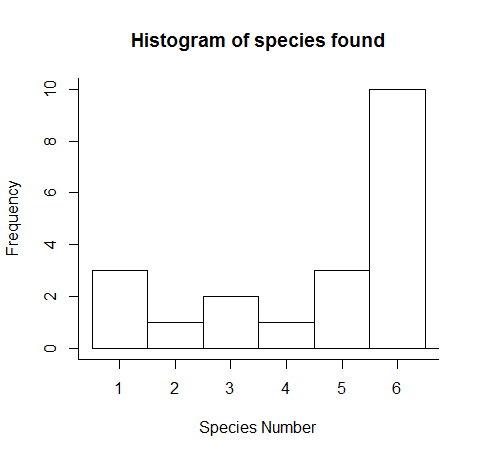
\includegraphics[keepaspectratio]{species-richness/data-image/site-1-histogram.png}}

}

\caption{\label{fig-site-one-histogram}Abundance of the first six
species of dragon recorded on the Island of Dragons, on the rocky beach
(site 1).}

\end{figure}%

We walk up the beach and up a steep valley that leads into the interior
of the island, and stop to take another sample. There's a lovely view
back to the sea, but we are far enough from the beach, and have
travelled rapidly enough, that we are confident that we will only see
different individuals here. At site 2 (the valley), we are still
surrounded by purple dragonflies, and indeed five of the six species we
saw on the beach are also visible here. However, in the undergrowth at
the side of the path we find a deep blue dragon snake, and in one of the
trees there is a violet humming dragon. We get very excited; they are
extremely rare. In the valley (site 2) we have found seven species in
total, two of which are new to the study. Our cumulative species count
goes up from six to eight.

We take another short hike and emerge at the top of the valley, at the
side of a scree slope. The purple dragonflies are menacing us, but
no-one has been bitten yet. We are surprised not to see more than one
yellow-bellied rock dragon, but there is a good show of turquoise cliff
dragons. After a few minutes we spot a pink slow-dragon basking on a
flat rock. That gives us four species for the site, one of which is new
to our set of observations, and brings our total species count up to
nine species.

We keep moving across the island, taking observations and counts in
multiple locations. Our number of new species keeps increasing: by the
fifth site (on the far side of Spiny Mountain, back in the scrub just
above the treeline), we have seen 12 different species, although each
site has an average of about six species within it. We take a lunch
break and start to plot the number of unique species recorded against
the number of samples that we've taken (Figure~\ref{fig-site-5}).

\begin{figure}

\begin{minipage}{0.50\linewidth}

\pandocbounded{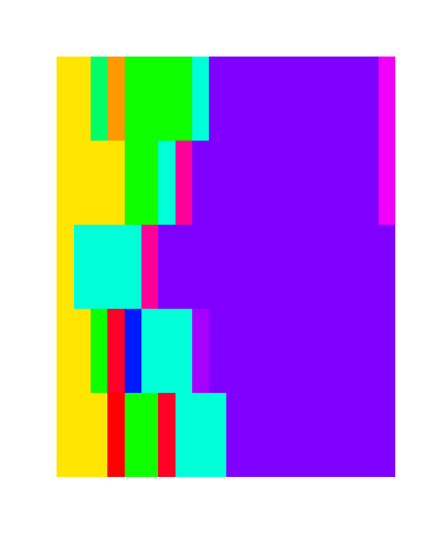
\includegraphics[keepaspectratio]{species-richness/data-image/site-5-heatmap.png}}

\end{minipage}%

\end{figure}%

Fired up by sandwiches and scroggin, and aided by a three day camping
trip, we launch ourselves into more sampling. We repeat our counts at
100 sites across the island, in the hope that we will see patterns
emerging in the dataset. There is likely a dominant species in this
community -- one species turning up in all of our samples.

By the 100th site, we have found 31 unique species even though each site
has an average of six to ten species each (Figure~\ref{fig-site-100}).
The rapid rise in the number of species at the start is followed by a
long period of plateauing at approximately 26 species. Eventually we
find a few rarer species; the discovery of an azure dragontoad hiding
under a waterfall and the lime green wyvern will definitely help us get
funding for the next field trip.

\begin{figure}

\begin{minipage}{0.50\linewidth}

\pandocbounded{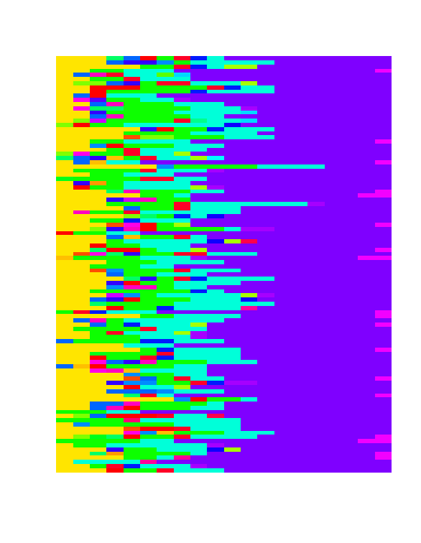
\includegraphics[keepaspectratio]{species-richness/data-image/site-100-heatmap.png}}

\end{minipage}%

\caption{\label{fig-site-100}\pandocbounded{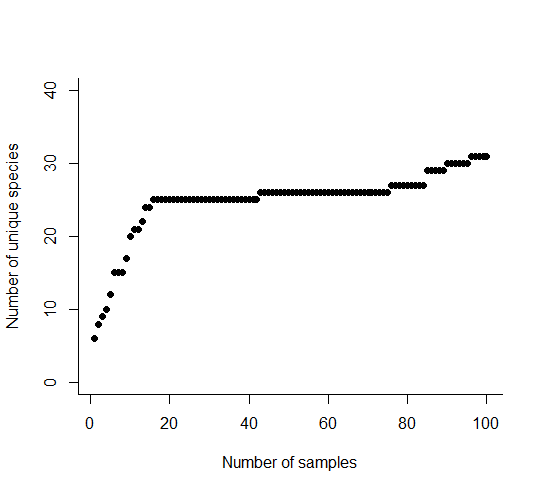
\includegraphics[keepaspectratio]{species-richness/data-image/site-100-curve.png}}
The species accumulation curve after 100 samples: purple dragonflies
continue to be the most common species, but there are a lot of rare
dragons and if we had given up after 60 samples we would have observed
only 26 of the 31 we eventually found.}

\end{figure}%

The problem with our records is that they produce a `noisy' curve. The
individual sites with particularly rare species or even just a lot of
species have the potential to affect the shape of the curve simply by
the order in which we sampled them. If, for example, the weather had
been different, or we had chosen a different path around the island, the
order of the sampling regime would have been different and our species
accumulation curve could have looked very different. This curve is known
as a `collector's curve' -- it is reflecting the one particular way in
which the data were collected

\section{Reordering, randomisation, and
rarefaction}\label{reordering-randomisation-and-rarefaction}

\subsection{Reordering}\label{reordering}

Reordering the data differently produces a similar, but not identical,
species accumulation curve. We see the same characteristic curve with a
rapid rise at the beginning, followed by a slowing down, but the
reordering doesn't necessarily get the long plateau that we saw in our
walk around the Island of Dragons (Figure~\ref{fig-reordered-curve}).
The end point is the same, but the curve is shaped differently. However,
we are not getting much of use from a single reordering; we're just
going on a walk across the island using a different route. What we
really want to know is, for a walk in any possible direction around the
island, how many dragon species should we expect to see on average after
1, 10, 25 sampling sites?

\begin{figure}

\centering{

\pandocbounded{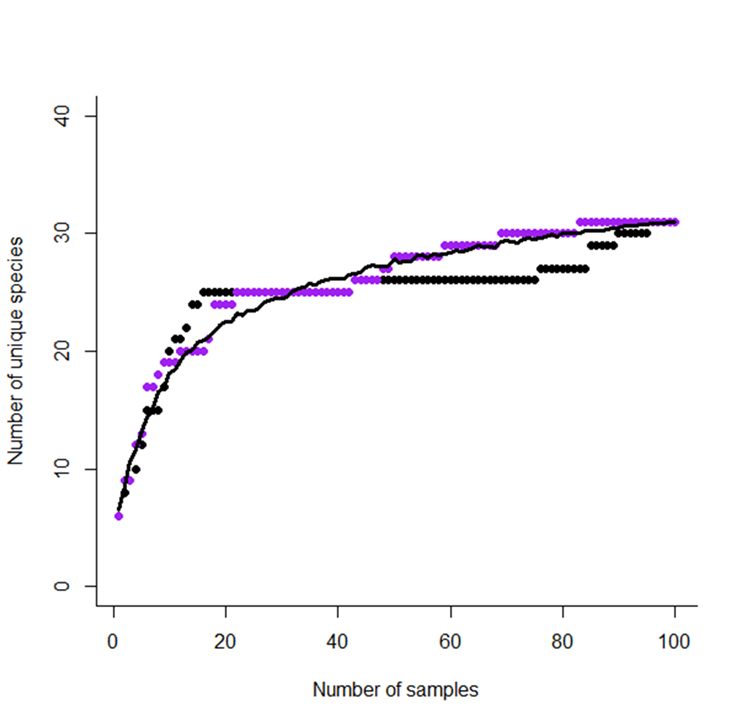
\includegraphics[keepaspectratio]{species-richness/data-image/reordered-species-accumulation-curve.png}}

}

\caption{\label{fig-reordered-curve}}

\end{figure}%

\subsection{Randomisation}\label{randomisation}

To try and reduce the bias that can come from the specific order in
which we collect our data, we can re-order the data multiple times
through a process called randomisation. We can then work out the mean
number of observed species for a given sampling effort from lots of
different sample orders, and we produce a smooth curve.

Randomisation is a tool that helps us to smooth out the data, and helps
us to compare between communities. It is affected by the relative
abundance of individuals of species in your community.

A short hop over the sea from the Island of Dragons lie Scaly Isle and
Spiny Isle. These are both extremely well documented lumps of land, and
the last population count indicated that both islets hold 50 individuals
of five species of small, cold-blooded dragons
(Figure~\ref{fig-scaly-spiny}). However, Scaly Isle is a very even
community, with all species present occurring at the same frequency.
Spiny Isle on the other hand is a very uneven community, with a lot of
individuals from one species and very few individuals from the other
species.

\begin{figure}

\begin{minipage}{0.50\linewidth}
\pandocbounded{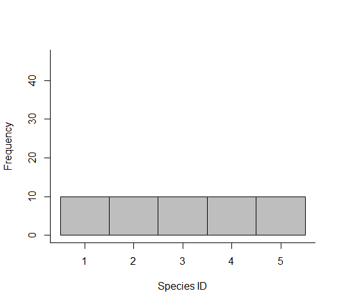
\includegraphics[keepaspectratio]{species-richness/data-image/scaly-isle-even.png}}\end{minipage}%
%
\begin{minipage}{0.50\linewidth}
\pandocbounded{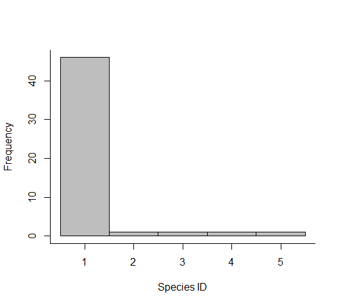
\includegraphics[keepaspectratio]{species-richness/data-image/spiny-isle-uneven.png}}\end{minipage}%

\caption{\label{fig-scaly-spiny}The distribution of 50 individuals among
five species on Scaly Isle (left) and Spiny Isle (right).}

\end{figure}%

When we visit, we record the individuals one at the time in the order
that we see them. On Scaly Isle, we meet all five species very quickly:
our collector curve gets us to five species by the time we've sampled
individual number 12, and we have reasonable confidence that there
aren't any more to find after sampling half of the population
(Figure~\ref{fig-scaly-spiny-collector-curves}). On Spiny Isle, we don't
find all species until we sample the 40th individual, and cannot expect
to do so with any reasonable confidence until we have sampled them all.
If we didn't know that there are only 50 individuals, we might even
conclude that there are more species still to discover.

\begin{figure}

\centering{

\pandocbounded{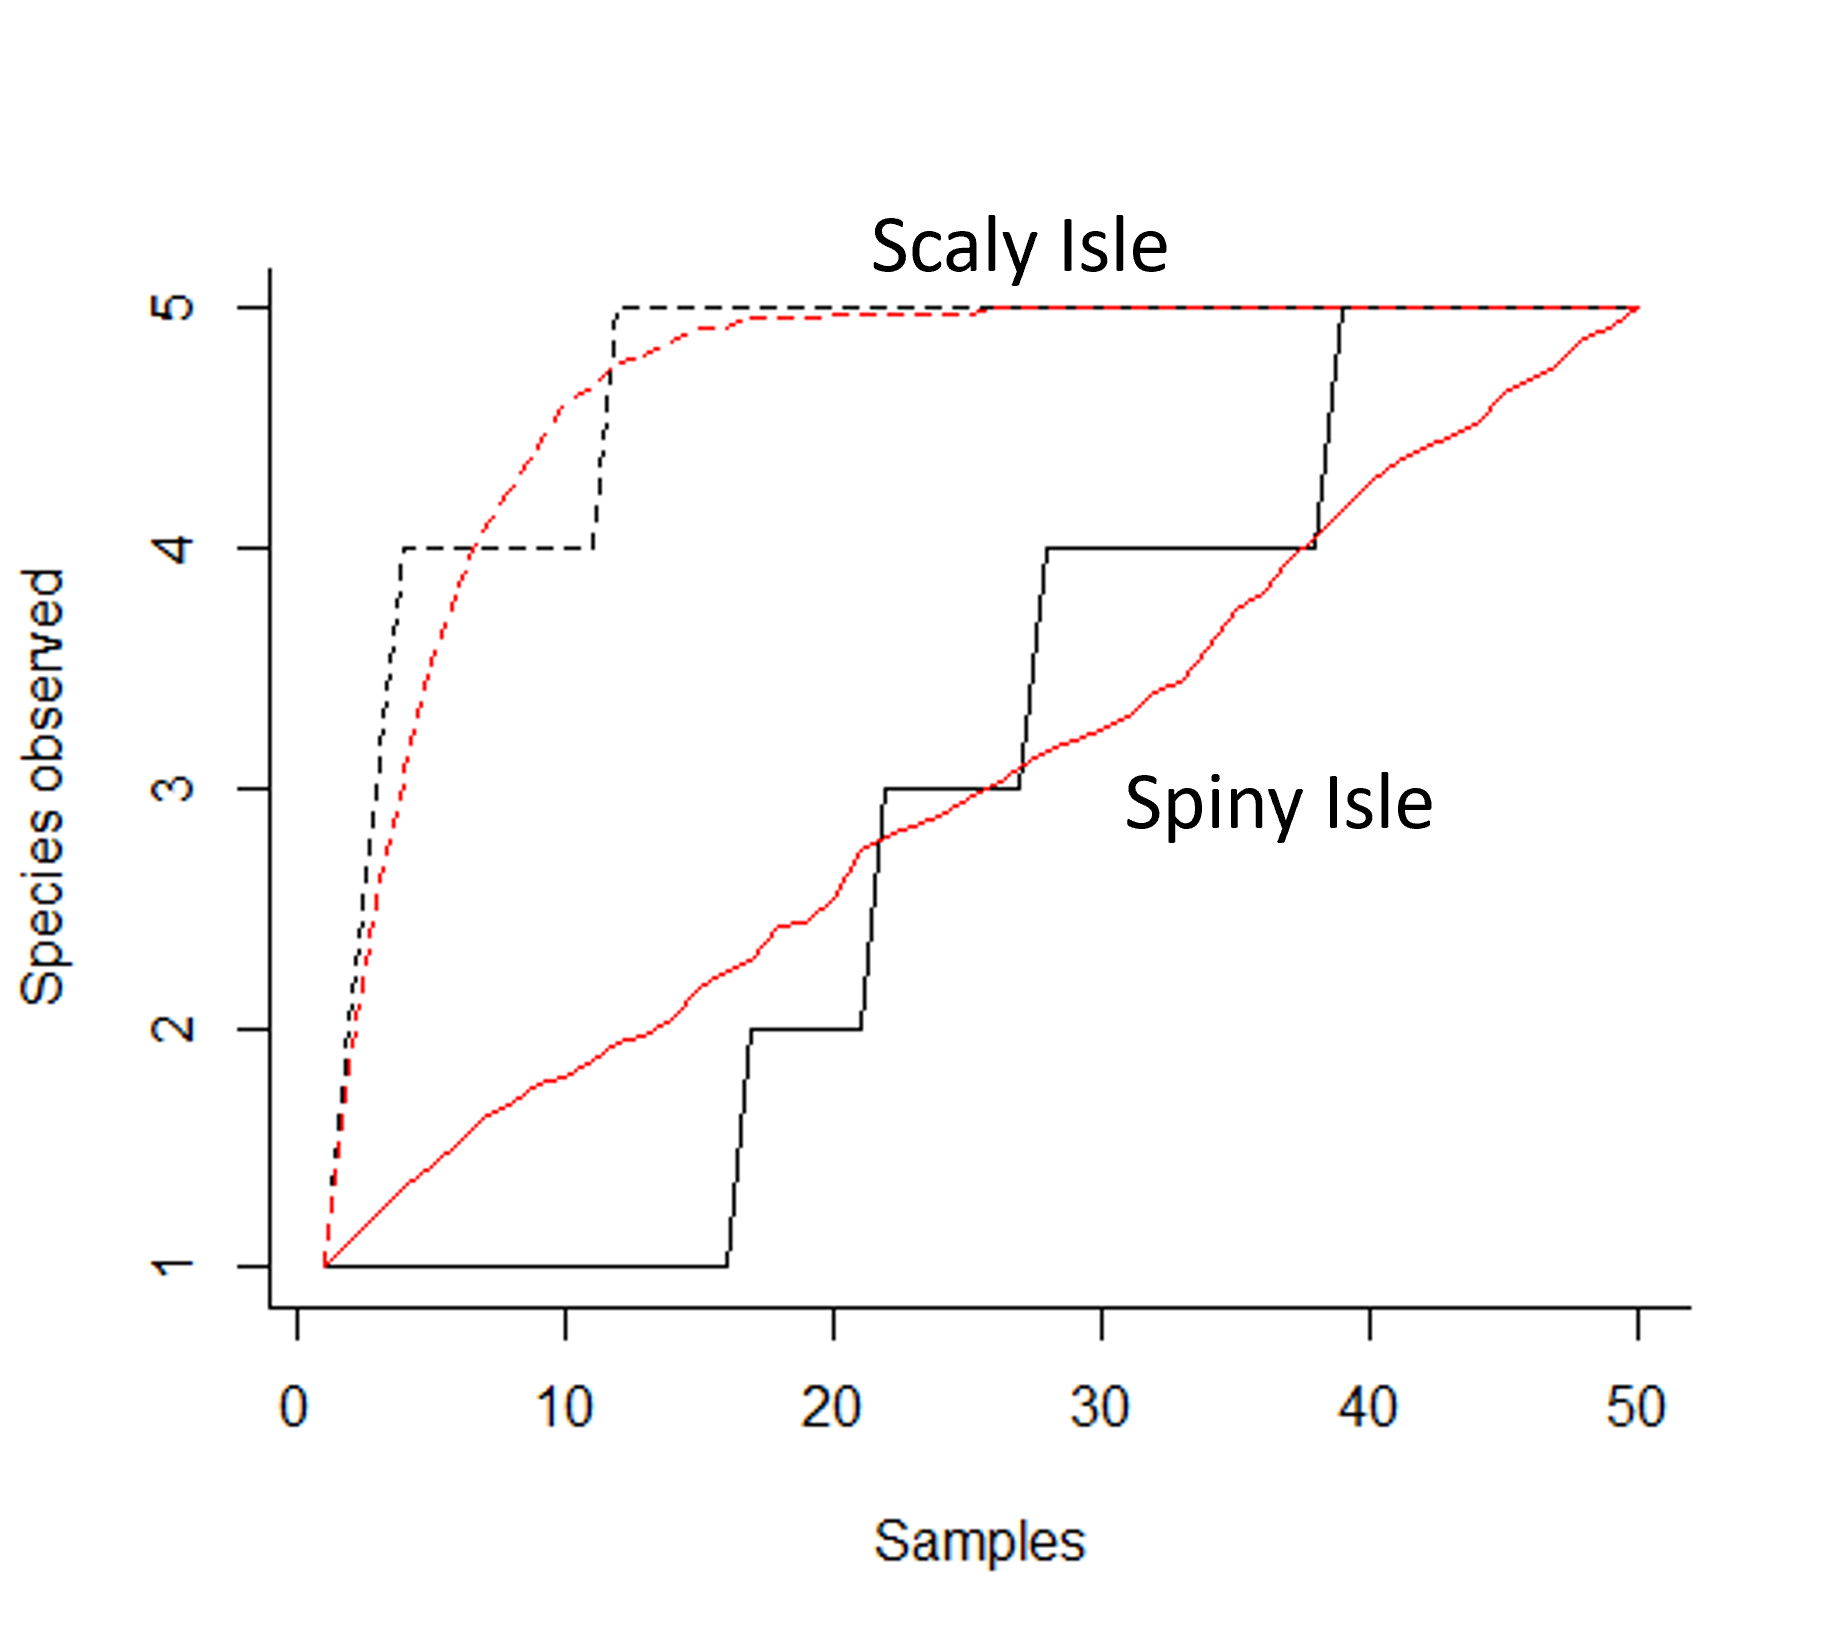
\includegraphics[keepaspectratio]{species-richness/data-image/scaly-spiny-collector-curves.png}}

}

\caption{\label{fig-scaly-spiny-collector-curves}Collector curves
(black) and randomised curves (red) for Scaly Isle (dashed lines) and
Spiny Isle (solid lines). Using the randomised curves, we expect to
encounter all five species by the 25th individual on Scaly Isle, where
the species are equally well represented in the community. However, we
cannot be confident that we have found all five species on Spiny Isle
until we have sampled all 50 individuals, because four of the species
are so (relatively) rare.}

\end{figure}%

Why randomise? When you have species data from different communities
with similar sampling effort, randomization gives you a smooth curve
that is easier to compare between communities, and less subject to
random biases. The shape of the species accumulation curve helps us to
distinguish between communities. Randomisation gives us more confidence
that the differences are real, and helps us draw conclusions about the
species richness of a more fully surveyed community
(Figure~\ref{fig-randomisation-rarefaction-info}): if the sampling
effort doubled, how would that affect the observed species richness?

Because randomisation keeps the collection of individuals and species
found in any one site or sample together (just reorders these), it
preserves the spatial differences and distribution of species among
sites. For example, if some sites are particularly different, e.g.~one
site only has very rare individuals, or where there's a large jump in
diversity in a single site, then it will appear in your randomized data,
acknowledged in the width of the confidence intervals around the mean.

\subsection{Rarefaction}\label{rarefaction}

Rarefaction is a process that allows us to use information about species
and samples to estimate the species richness of a smaller sample. It
uses information about the abundance of each of the species in an
observed sample to calculate the chance of observing some number of
species in a smaller sample
(Figure~\ref{fig-randomisation-rarefaction-info}). For example, on the
Island of Dragons, we collected data from one hundred sample sites. If
we want to compare that to a historical study that only sampled fifty
sites, or perhaps compare species richness on this island with another
further up the coast, we can use a process called rarefaction.

\begin{figure}

\centering{

\pandocbounded{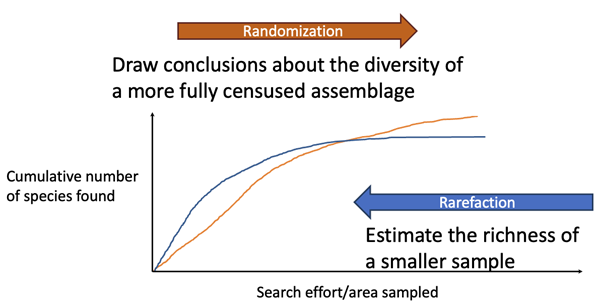
\includegraphics[keepaspectratio]{species-richness/data-image/randomisation-rarefaction-infographic.png}}

}

\caption{\label{fig-randomisation-rarefaction-info}Species accumulation
curves can be constructed for increasing sampling effort. Randomisation
helps to draw robust conclusions about the species richness of the
`complete' community, by inferring from left to right on the graph what
may happen if we keep sampling. Rarefaction works from right to left to
infer the likely species richness of a sample smaller than the whole.}

\end{figure}%

Rarefaction can be carried out using the following equation. You don't
have to memorise it, or even calculate it yourself, but it will help you
understand how it works if you can see how it is put together:

\$\$ E(S\_n) = K - (\{N \over n\})\^{}\{-1\} \Sigma\_\{i = 1\}\^{}\{k\}
(\{N - N\_i \over n\})

\$\$

Here, the number of unique species in any subsample of size \emph{n} is
\((S_n)\). The expected number (on average) of unique species in a
subsample of size \emph{n} is \(E(S_n)\). This is equal to the total
number of unique species in the whole sample (\emph{K}), minus the
chance that any or each species is not represented. This is calculated
taking into account:

\begin{itemize}
\tightlist
\item
  How many ways there are of choosing n individuals from your total N
  individuals (``N choose n''): \(({N \over n})\)
\item
  How many ways there might be of doing this for every one of the
  \emph{K} species (\(\sum_{i = 1}^{k}\))
\item
  And, if the individuals from species \emph{i} are removed
  (\(N - N_i\)), how many ways are there of picking \emph{n} individuals
  from the remainder: \(({N - N_i \over n})\)
\end{itemize}

Thus, the equation accounts for the problem that if you have lots of
rare species, it is fairly easy to pick a sub-sample and miss some of
your species. If your community is quite even, it's less easy to avoid
those. Our understanding of commonness and rarity of species from the
relative abundance of the larger sample allows us to `backtrack', and
say that if we only sampled 50\% of the community, how many species are
we likely to find?

\chapter{Case study: breeding bird
censuses}\label{sec-bird-survey-case-study}

James and Rathbun (1981) carried out 37 surveys of breeding birds in the
US and Canada, recording the number of breeding pairs of birds in each
area, what species the breeding pairs were, and information about the
local landscape. They were interested in how the 37 communities differed
in organisation and structure across the habitats: however, it's also
clear that the sampling effort across the sites varied. We will pick
three sites of interest to explore in more detail
(Table~\ref{tbl-bird-survey-data}).

\begin{longtable}[t]{llll}

\caption{\label{tbl-bird-survey-data}Details of three sites from James
and Rathbun (1981).}

\tabularnewline

\\
\toprule
 & Site 2 & Site 6 & Site 9\\
\midrule
Number of breeding pairs & 54 & 100 & 50\\
Number of species & 20 & 24 & 14\\
Size of site (ha) & 6 & 11.6 & 12.0\\
Habitat & Tulip tree-beech-hickory & Oak-beech & Mature jack pine-birch\\
\bottomrule

\end{longtable}

Our three sites have three different habitats, on different size plots,
and have recorded different species richnesses from different numbers of
breeding pairs. How could we use rarefaction to determine if these three
sites have the same species richness as a function of sampling effort
(measured by number of individuals)?

In the oak-beech forest at site 6, there were 24 bird species spread
across 100 breeding pairs (Table~\ref{tbl-bird-survey-data}). With our
rarefaction equation, we can ask -- if only 50 pairs were sampled, how
many species would we expect to have been found at this site? For this,
we need the rank abundance data from the site
(Figure~\ref{fig-bird-survey-abundance}), which shows that some species
are quite rare: we have seven species represented by only 1 breeding
pair. There are many common species (more than 5 breeding pairs) at the
site.

Applying the rarefaction equation to these numbers suggests that we'd
expect to see 18.5 species if we halved our sample effort and only
recorded 50 breeding pairs. This 18.5 isn't half of the original 24
species represented by 100 breeding pairs, but does represent
approximately 2/3rds of them. Rarefaction also lets us calculate a
standard deviation that helps us be 95\% sure that halving sample effort
would let us observe between 15 and 21 species at the site.

\begin{figure}

\centering{

\pandocbounded{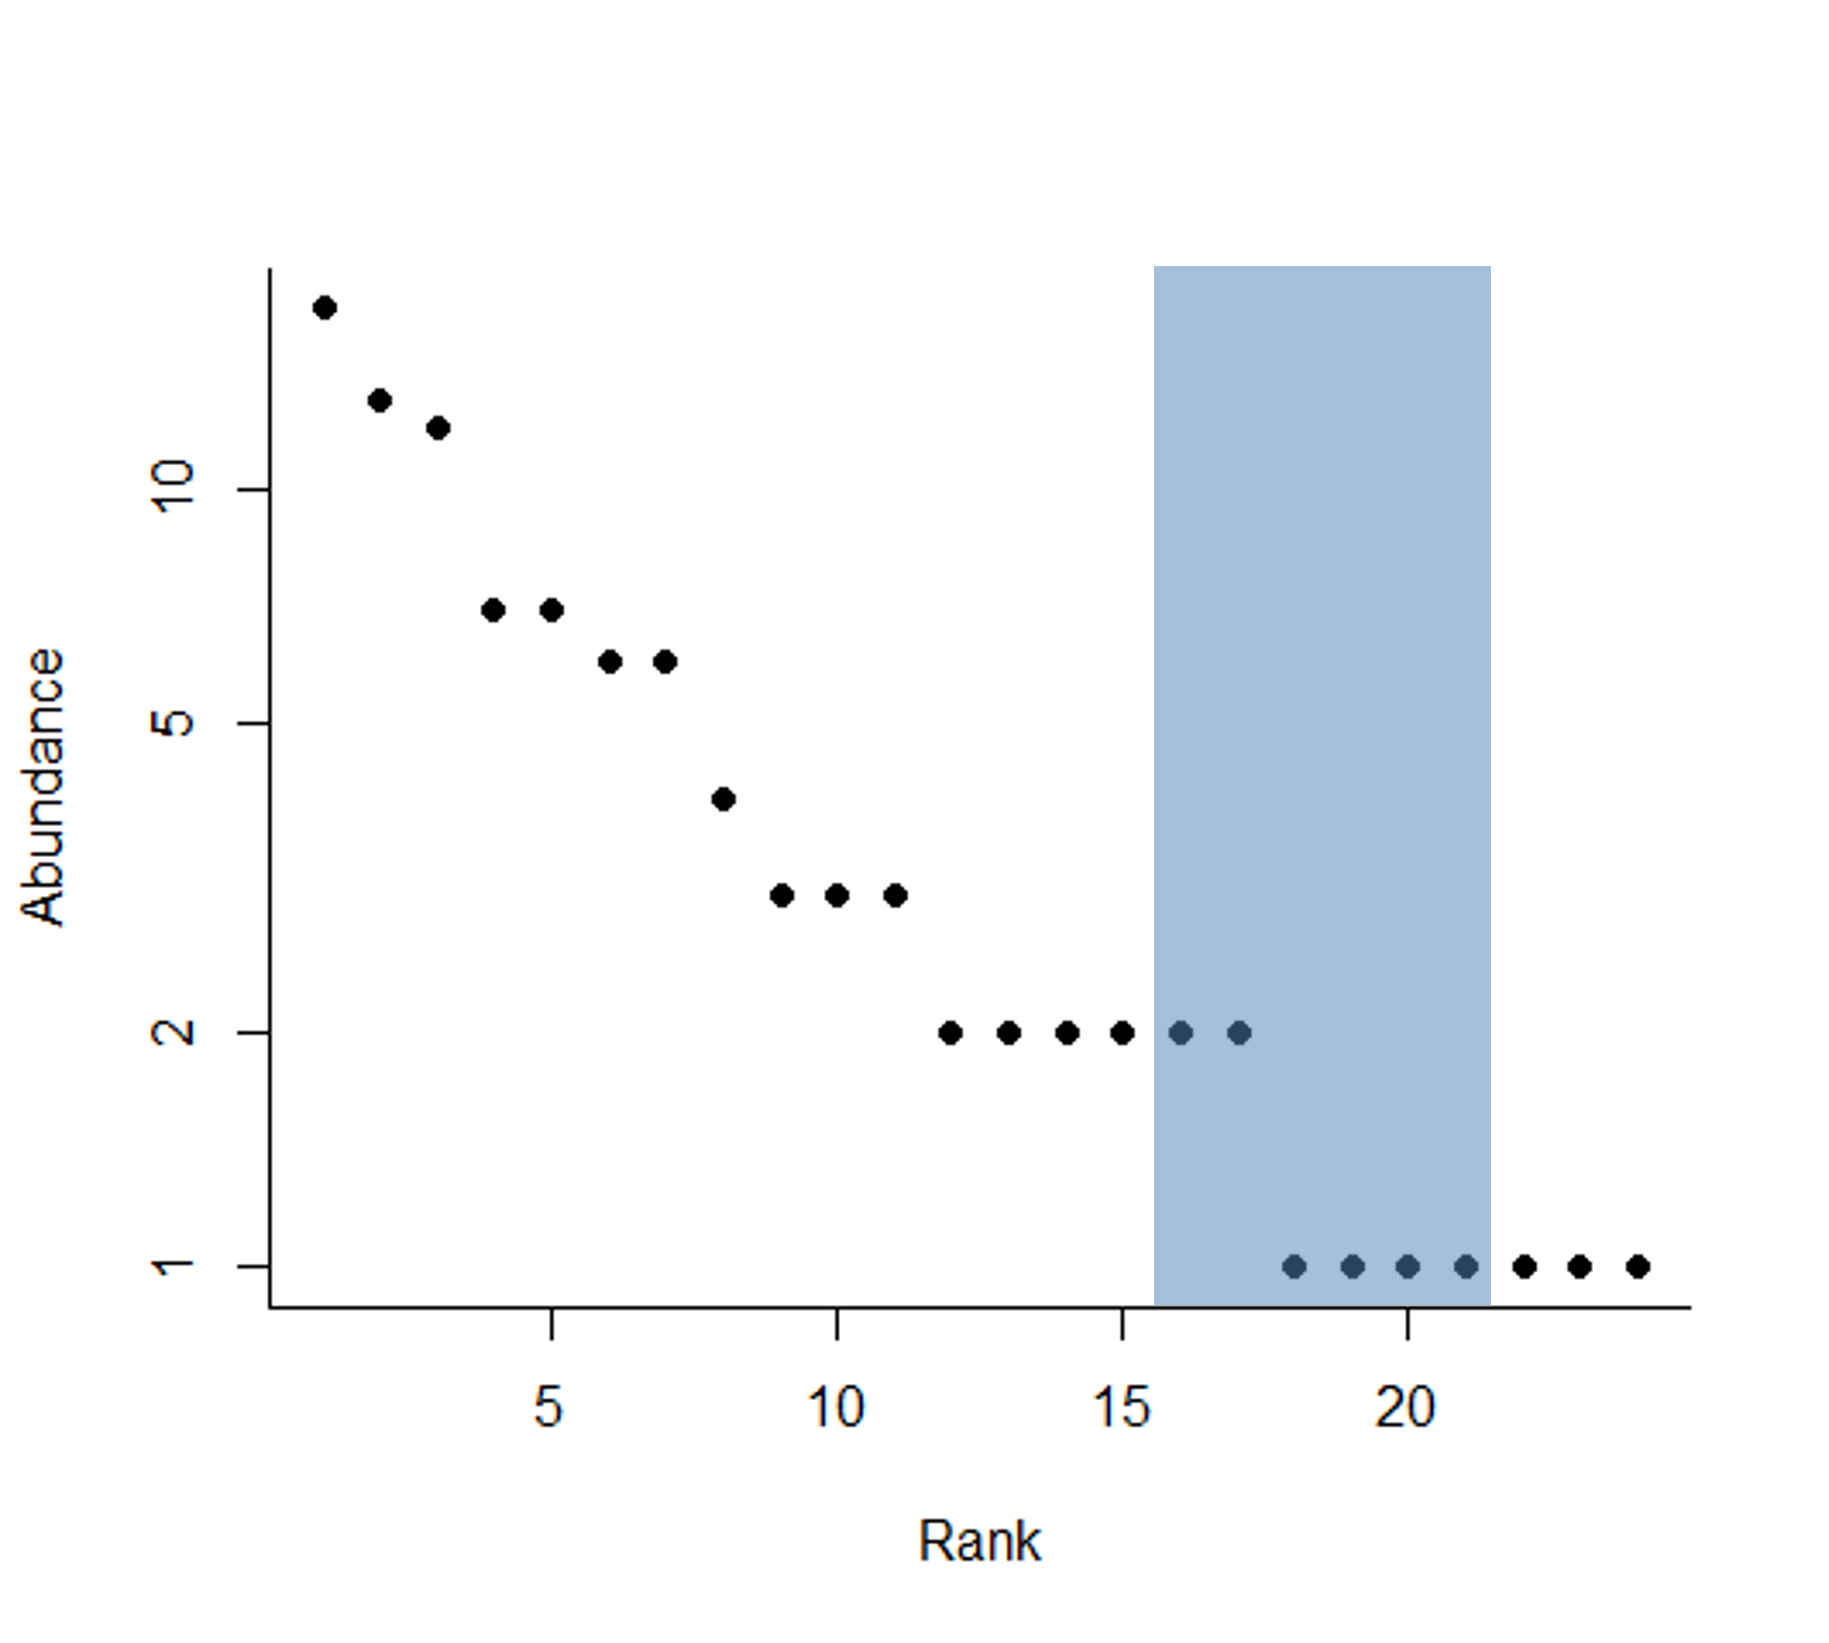
\includegraphics[keepaspectratio]{species-richness/data-image/bird-survey-abundance.png}}

}

\caption{\label{fig-bird-survey-abundance}}

\end{figure}%

Repeating this process for all 37 of the breeding bird censuses allows
comparison across all of the sites and sampling efforts
(Figure~\ref{fig-bird-survey-rarefied}). We can conclude that sites 2
and 6 are of similar species richness, after adjusting for sampling
effort. However, site 9 appears to be significantly less diverse.

\begin{figure}

\centering{

\pandocbounded{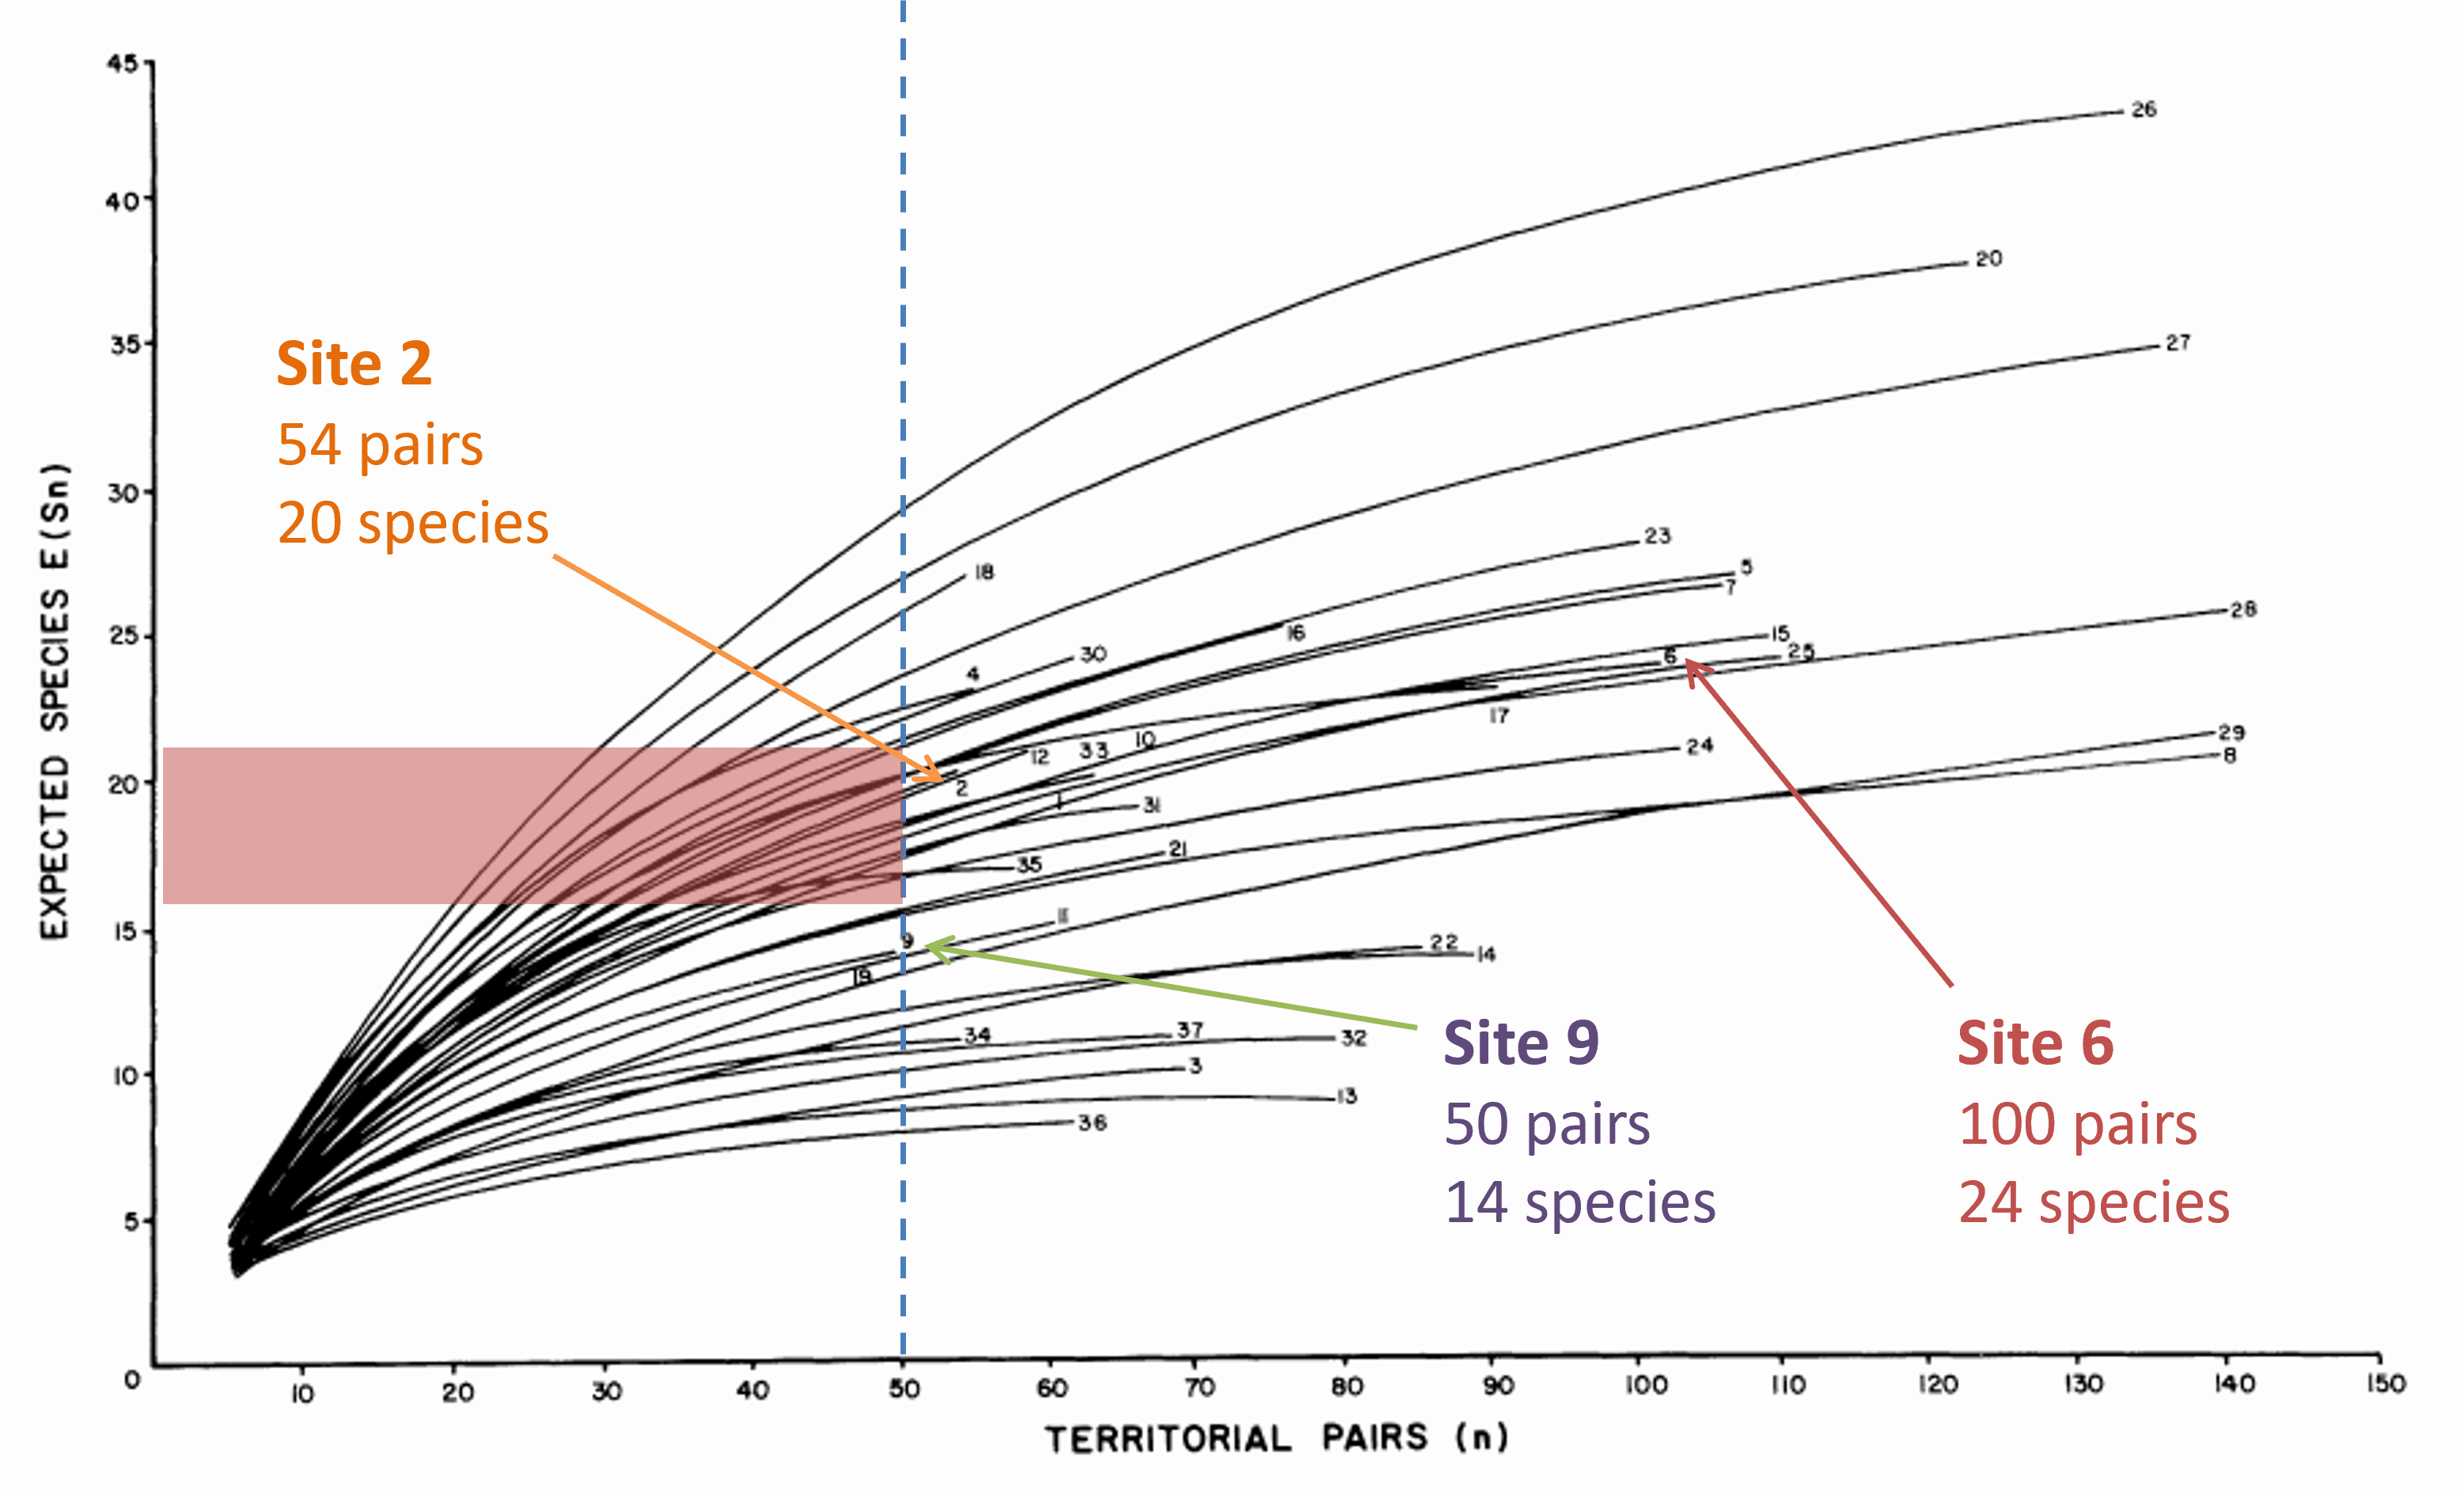
\includegraphics[keepaspectratio]{species-richness/data-image/bird-survey-rarefied-estimate.png}}

}

\caption{\label{fig-bird-survey-rarefied}Rarefied estimate for expected
number of species given the number of breeding pairs recorded, for all
sites. The total number of pairs and species observed at a site can be
read from the top right of each line; e.g.~site 26 has the highest
number of species but sites 8, 27, 28 and 29 had more breeding pairs.
Site 9 had the lowest number of breeding pairs (50, highlighted with the
blue dashed line) observed in one survey. The expected number of
breeding pairs at Site 6 if 50 breeding pairs were observed is
highlighted by the orange line (mean) and 95\% confidence interval
(orange rectangle). Site 2 crosses the 50-breeding-pairs line within the
confidence interval. Site 9 falls below it.}

\end{figure}%

So rarefaction has allowed us to compare species between samples with
different efforts and sampling sizes to \textbf{describe} comparable
differences between the communities. We now want to \textbf{explain} the
differences between sites.

Remember that each of the study areas was a different size, as well as
having a different number of breeding pairs of any species? This means
that each community was also at a different density. We can calculate
the area occupied by 50 breeding pairs (assuming that the pairs are
evenly distributed in space) so see what the effect of density might be
on expected species richness (Figure~\ref{fig-bird-species-expected}).
There is a relationship between territory density and species richness,
and this is broadly related to the habitat type. Sites 2 and 6 are both
deciduous habitats with a similar expected species richness and density:
their 50 pairs occupy a fairly small area with a high species richness.
Site 9, on the other hand, is lower in species richness and density. It
sits in a transition space on the graph between deciduous forest and
coniferous-deciduous habitats. We now see that second growth habitats
are expected to have higher species richness, and while tundra, desert
and coniferous habitats have lower species richness, coniferous areas
operate at lower density as well.

Rarefaction has allowed us to make this direct comparison, and draw out
more information about factors impacting the communities of bird
species.

\begin{figure}

\centering{

\pandocbounded{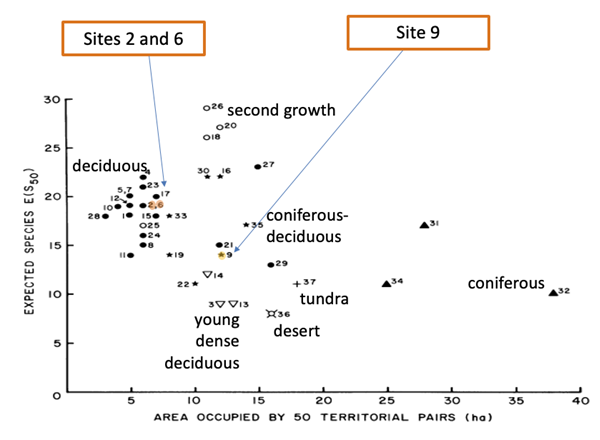
\includegraphics[keepaspectratio]{species-richness/data-image/bird-survey-expected-numbers.png}}

}

\caption{\label{fig-bird-species-expected}}

\end{figure}%

\section{References}\label{references-2}

James, F. C., \& Rathbun, S. (1981). Rarefaction, Relative Abundance,
and Diversity of Avian Communities. The Auk, 98(4), 785--800.
http://www.jstor.org/stable/4085899

\chapter{Species richness: A
summary}\label{sec-species-richness-summary}

The patterns of species accumulation over increasing sampling effort
encapsulate different processes and scales of observation. Three key
questions to bear in mind are: * How many species are found on average
in one sample? * How many species coexist in the community at large? *
How much does the relative abundance of species vary between any pair of
samples in your dataset, or between communities that you want to
compare?

In the next chapter we will build on these ideas to explore how we can
estimate `true' species richness from observed species using different
methods, and combine species relative abundance with species richness to
measure ecological diversity.

\part{Diversity}

In the last chapter, we moved on from counting individuals as members of
populations, to think about collections of populations that are all
present in the same place at the same time, as ecological communities.
We can estimate how many species are present by observing species
richness, and during that process, we notice that the number of
individuals of each species differs: some are more common, and others
are rarer. The composition, or make-up, of the community affects
estimates of species richness, and in turn these are affected by
sampling effort.

In this chapter, we will explore the concept of rank abundance in more
detail, using models to describe different patterns of species abundance
and evenness (Chapter~\ref{sec-abundance-and-evenness}) and true species
richness (Chapter~\ref{sec-patterns-species-richness}). We'll then
combine these ideas with ecological diversity indices
(@sec-ecological-diversity).~

This is a longer chapter than usual, but your focus this week should be
on understanding the higher level concepts highlighted in the summary at
the beginning of each subsection (TL;DR). There will be technical
support available if/when you want to start using these for your
fieldwork. In the workshop this week, you'll calculate some indices of
ecological diversity and start to use a variety of metrics for diversity
to compare sites and better understand why species are where they are.~

\chapter{Patterns of species abundance and
evenness}\label{sec-abundance-and-evenness}

\section{Too Long; Didn't Read (TL;DR)}\label{too-long-didnt-read-tldr}

What's the take home message for
Chapter~\ref{sec-abundance-and-evenness}? Rank abundance, or species
abundance, tells us how individuals are distributed across species in a
community. There are many mathematical models developed to describe the
different shapes seen in the curve made by a rank abundance plot, where
the number of individuals in each species are plotted from most common
to rarest (x axis) on a log scale (y axis). We can fit models to
observed data: here, we are asking whether the expected values produced
by the model are a good match to the observed values, like we did with
the Poisson distribution to assess whether \emph{Plantago lanceolata}
were randomly distributed in space in week 2. The best fitting species
abundance model tells us that, whatever the assumptions sitting behind
that model might be, this is a credible explanation for why the
community looks the way it does. When we have multiple communities, we
can compare the parameters of the best fitting models or different model
types to better understand why the communities are similar or different.

\section{Why use models?}\label{why-use-models}

Within any community of interest (whether at the large scale or the
microscopic), we want to describe the relationship between the number of
species and the number of individuals in those species. This is the
relative abundance of species that make up a community. Rank abundance
models help us to understand both species richness, and the evenness of
the distribution of those species.

As ecologists, we need models to use as tools to produce realistic
rank-abundance patterns. These models help us to describe and explain
the processes that help to form or change a community. At a simple
level, the shape of the line of the rank abundance plot is a descriptive
model. For example, Bazzaz (1975) created rank abundance plots for a
number of species growing in fields, where the number of years for which
the fields had been left fallow varied from one to 40 years
(Figure~\ref{fig-plant-succession}). The plants are identified as herbs,
shrubs and trees, and the index of abundance is relative cover, rather
than biomass or abundance. Take a look back at Chapter 2 to reacquaint
yourself with measures for plant abundance if you need to: counts,
masses, and areas, are all acceptable for this type of plot.

Bazzaz (1975) shows that in early succession, i.e.~the fields left
fallow for only a short period of time, rank-abundance can be described
by a relatively straight line. There are few species in total, and they
are mostly herbs; there is a high degree of dominance. As time
progresses and succession continues, trees and shrubs begin to appear,
and in the 25 to 40 year rank abundance plots you can see both a higher
species richness, and a more even community structure, although some
species are still considerably more abundant (or dominant) than others.

\begin{figure}

\centering{

\pandocbounded{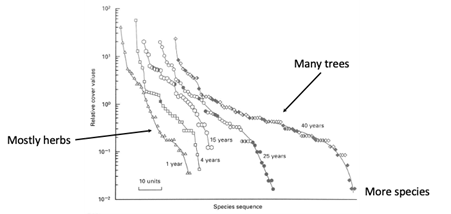
\includegraphics[keepaspectratio]{diversity/data-image/bazzaz.png}}

}

\caption{\label{fig-plant-succession}}

\end{figure}%

In the previous chapter, we saw a similar pattern of change in rank
abundance moving from the straight line of the species poor boreal
forest through temperate deciduous and tropical semideciduous forests
towards the species rich and relatively even tropical rainforest.

Rank abundance can help us describe patterns, and change in patterns,
over time and space. To help to explain these, we can develop models
that produce different rank abundance patterns as a result of underlying
processes. When we fit models to real world data, we can estimate
parameters and goodness of fit, to see which models are a reasonable
description of the community structure. We can then use these models as
evidence to suggest which process gave rise to the community that we
have observed.

\section{Species abundance models}\label{species-abundance-models}

There are two broad categories of species abundance models:
\textbf{statistical} and \textbf{biological}. * Statistical models such
as the log species \textbf{describe} the observed patterns of rank
abundance, and the parameters of these models can tell us useful
information such as the mean or variance of rank abundance within the
community. * Biological (or theoretical, or mechanistic) models, such as
the geometric series or niche apportionment, \textbf{explain} the
observed pattern of rank abundance as the result of a process. The
parameters of these models therefore tell us something about how the
community arose.

When we are referring to species abundance models, there is some common
terminology: * \emph{S} is (usually) the total number of species.
However, sometimes this refers to the number of sites. When you write
about models, always define your terms when you use them, to avoid
ambiguity. We will endeavour to do the same here. * \emph{N} is the
total number of individuals * \(P_i\) is the proportion of individuals
that species \emph{i} contributes to the total (relative abundance) *
\(S_n\) is the number of species with \emph{n} individuals (the
frequency of species in relation to abundance)

Within our statistical and biological models, we can also ask whether
the patterns of distribution are \textbf{stochastic} or
\textbf{deterministic} (Figure~\ref{fig-model-examples}).

\begin{figure}

\centering{

\pandocbounded{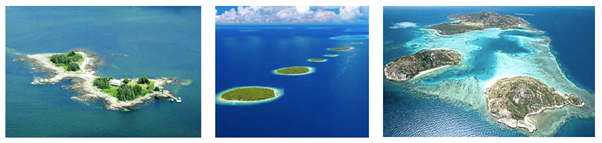
\includegraphics[keepaspectratio]{diversity/data-image/example-islands.png}}

}

\caption{\label{fig-model-examples}. In a deterministic model, there is
one rule to distribute individuals among islands, e.g.~as a function of
their number, size, habitat or distance from the mainland. In a
stochastic model, there is a random variable at play and the rules are
probability-based rather than perfectly repeatable. This is still a
function of the driving factors such as number, size, habitat or
distance, but two islands with equal properties are not guaranteed to
have the same community composition.}

\end{figure}%

Here follows a handful of common species abundance models, with case
studies for when they have been used to understand change or formation
of communities. You do not need to memorise equations or be able to
apply these from scratch. The main learning outcome is to appreciate
that there are many different models, and each one has different
underlying assumptions or implications for the community that it best
fits.

\section{Statistical models}\label{statistical-models}

\subsection{Log series}\label{log-series}

One of the first statistical species abundance models was developed by
Fisher \emph{et al.} (1943). The log series model gives the number of
species within a community that are predicted to have \emph{n}
individuals (\(S_n\)):

\[
S_n = {\alpha x^n \over n}
\] The number of species with an abundance of \emph{n} (\(S_n\)) is
equal to a positive constant derived from the sample data (\(\alpha\) :
alpha) multiplied by a positive constant also derived from sample data
(\emph{x}), divided by the number of individuals that you are interested
in (\emph{n}). What does this mean in practice? If we wanted to find the
number of species with 1, 2, 3, or more individuals, all the way up to n
individuals, we would need to calculate the sequence:

\[
\alpha x, {\alpha x^2 \over 2}, {\alpha x^3 \over 3}, {\alpha x^4 \over 4}, ... , {\alpha x^n \over n}
\] In practice, the value of \emph{x} tends to be close to one. This
means that at the beginning of the sequence (n=1), \(\alpha\) is roughly
the number of species with 1 individuals. This can be taken as a measure
of the number of rare species.

As we approach the other end of the sequence, the number of individuals
within a species increases (i.e.~as it becomes more common), and the
expected number of species with \emph{n} individuals decreases. This
means we may only get one or two species with a high number of
individuals, or only one or two common species.

\subsection{Case study: log series in Indonesian
butterflies}\label{case-study-log-series-in-indonesian-butterflies}

Hill et al.~(1995) compared the species abundance of butterflies in
Buru, Indonesia, comparing logged and unlogged forest to determine if
the community structures differed with different levels of disturbance
(Figure~\ref{fig-hill-species-abundance-plots}). Unlogged communities
had more individuals and more species compared to the logged forest
regions (\textbf{?@tbl-butterfly\_data}). When a log series model was
fitted to the data, the alpha value from the unlogged forest (7.94) was
higher than that from the logged forest (6.99). Remembering that alpha
is a rough representation of the number of species with 1 individuals,
this implies that the unlogged communities have more rare species than
the logged communities.

\begin{figure}

\centering{

\pandocbounded{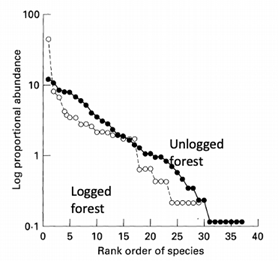
\includegraphics[keepaspectratio]{diversity/data-image/hill-species-abundance-plots.png}}

}

\caption{\label{fig-hill-species-abundance-plots}}

\end{figure}%

\begin{longtable}[t]{lll}

\caption{\label{tbl-butterfly-data}Observed number of species and
individuals, and best-fit parameters for the log series model, for
unlogged and logged forest (from Hill et al.~1995).}

\tabularnewline

\\
\toprule
 & Unlogged & Logged\\
\midrule
Number of species & 37 & 29\\
Number of individuals & 828 & 458\\
alpha & 7.94 & 6.99\\
x & 0.99 & 0.98\\
\bottomrule

\end{longtable}

\subsection{Log normal}\label{log-normal}

The log normal model for species abundance was devised by Preston in
1948. Rather than plotting the relative number of individuals by species
in rank order (as per a rank abundance plot), or calculating the exact
frequencies of species with abundance \emph{n} (as seen in the log
series), the log normal model looks at the distribution of individuals
amongst species using a histogram. In this histogram
(Figure~\ref{fig-species-abundance-histogram}), the y axis represents
the number of species. The x axis represents the number of individuals
in that species, and these are grouped together into classes called
octaves. The maximum number of individuals in each octave doubles as the
classes increase, so the lowest octave is the number of species with one
individual, then two individuals, then three or four individuals, then
five to eight individuals, and so on: the x axis is thus using a log
base 2 scale, and the species distribution should look approximately
normally distributed. The modal class (remembering that the `mode' is a
version of an average, like the mean or the median) is the class
containing the most common number of individuals per species
(Figure~\ref{fig-species-abundance-histogram}).

\begin{figure}

\centering{

\pandocbounded{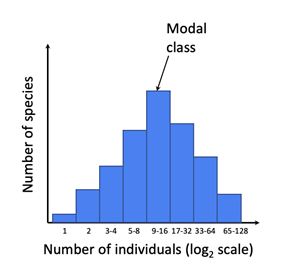
\includegraphics[keepaspectratio]{diversity/data-image/species-abundance-histogram.png}}

}

\caption{\label{fig-species-abundance-histogram}}

\end{figure}%

The log normal equation \(S(R) = {S_0}exp(-\alpha^2R^2)\) uses the
number of species within the modal class (\(S_0\)) and a function of the
variance of the distribution (\(\alpha =( 2\alpha^2 )^{-0.5})\)) to
calculate the number of species in any of the octaves to the left or
right of the modal class
(Figure~\ref{fig-log-normal-distribution-class}). The key takeaway is
that in a community that follows the log normal model, we expect to see
very few species with very few individuals, and very few species with a
large number of individuals.

\begin{figure}

\centering{

\pandocbounded{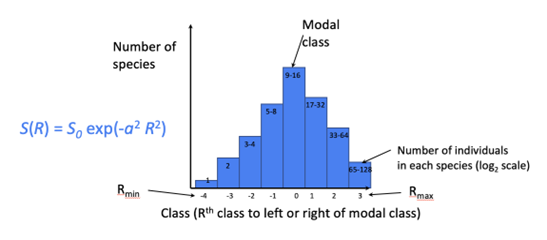
\includegraphics[keepaspectratio]{diversity/data-image/annotated-log-normal-distribution.png}}

}

\caption{\label{fig-log-normal-distribution-class}}

\end{figure}%

\section{Biological models}\label{biological-models}

Biological models for species abundance are based on the assumption that
an ecological community has a `multidimensional niche space' that is
divided up amongst the species who live there. The relative abundance of
species is used as a surrogate for niche size: for example, if half of
the individuals observed belong to one species, we assume that that
species occupies half of the available niche space. Biological models
describe a process of niche fragmentation or niche filling that results
in the observed species abundances. There are a number of different
models that describe different niche apportioning. We will consider a
handful briefly here.

\subsection{Geometric series}\label{geometric-series}

The geometric model is a very commonly seen biological model. It
describes a process by which species arrive at regular time intervals
into an unsaturated habitat (meaning there is still space left to
occupy). It is assumed that each species that arrives will occupy a
fixed fraction of the remaining niche space. The proportion of space
occupied by the \emph{i}th species to arrive is then:

\[
P_i = k(1 - k)^{i - 1}
\]

For example, if \emph{k} = 0.5, then the first species occupies \(P_1\)
= 0.5 or half of the niche. The second species to arrive gets \(P_2\) =
0.5(0.5) = 0.25 or quarter of the niche. The third species gets \(P_3\)
= 0.5(0.5)\(^2\) = 0.125 or an eight of the niche, and so on.

We see geometric mechanisms occurring in species-poor environments, or
in environments that are very early in succession processes. One species
is common and dominates the niche space, and the rare species very
rapidly become rare - and eventually are not present at all. Because the
ratio of each species to its predecessor is constant, when we plot the
log abundance-rank graph, we see a straight line.

\subsection{Case study: geometric series in the Park Grass
experiment}\label{case-study-geometric-series-in-the-park-grass-experiment}

The Park Grass experiment at Rothamsted is an experiment that was
initially designed to determine the effects of organic and inorganic
amendments and lime addition on grasslands used for hay. However, this
is a long term experiment that also includes information about how the
vegetation composition of the plots has changed over a number of years,
from 1856 to 1949 (Figure~\ref{fig-rothamsted-park-grass}). Since 1856,
we can see that the gradient of the rank-abundance lines has become
steeper, from which we can deduce that the value of k in the geometric
series model fitted to each set of data is increasing over time. That
indicates that the dominant (nominally `first arriving') species are
increasingly dominant in recent years compared to during the Victorian
origins of the experiment. As a result, species richness is lower, and
presumably competition (and competitive exclusion) is stronger.

\begin{figure}

\centering{

\pandocbounded{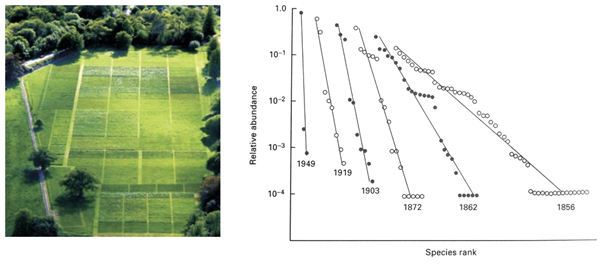
\includegraphics[keepaspectratio]{diversity/data-image/rothamsted-park-grass.png}}

}

\caption{\label{fig-rothamsted-park-grass}}

\end{figure}%

\subsection{Power fraction}\label{power-fraction}

Power fraction models are sequential breakage models in which niche
space is divided at random into pieces. An invading species (the
`colonists') will compete for the niche of a species already present,
and take a random proportion of that niche. The relative change of
choosing any one niche is a power function of the size of that niche:
that is, the relative chance of choosing a species with relative
abundance \(P_i\) is \(P_i^K\) where \(0 ≤ K ≤ 1\)
(Table~\ref{tbl-niche-colonisation}).

\begin{longtable}[t]{llllll}

\caption{\label{tbl-niche-colonisation}Diagram showing the chance of
choosing a niche for colonisation, if the original community has three
species occupying a quarter (0.25), a quarter (0.25) and a half (0.5) of
the niche space on arrival of the invader. The power fraction example
uses K = 0.5. The random fraction is the special case in which K = 0,
and each species has equal chance of being invaded regardless of space
occupied. The MacArthur fraction model is the special case in which K =
1, and the chance of being invaded is proportional to the niche space
occupied.}

\tabularnewline

\\
\toprule
 & Niche space occupied & Chance & 0.25 & 0.25 & 0.5\\
\midrule
 & Random fraction & \$P\{\_i\}\{\textasciicircum{}0\}\$ & 0.33 & 0.33 & 0.33\\
 & Power fraction & \$P\{\_i\}\{\textasciicircum{}K\}\$ & 0.293 & 0.293 & 0.414\\
 & MacArthur fraction & \$P\{\_i\}\{\textasciicircum{}1\}\$ & 0.25 & 0.25 & 0.5\\
\bottomrule

\end{longtable}

Power fraction models are pretty good at reflecting what's happening in
the real world: if you occupy a large niche, you're slightly more likely
to be invaded, but only slightly. This means that we see a long plateau
in the rank abundance plots, with a lot of species of approximately
similar relative abundance across the middle ranks
(Figure~\ref{fig-power-fraction-relative-abundance}). This plateau is
very flat where K=1, and becomes steeper as the K value gets closer to
0. Very species-rich assemblages tend to have a K value of less than or
equal to 0.2.

\begin{figure}

\centering{

\pandocbounded{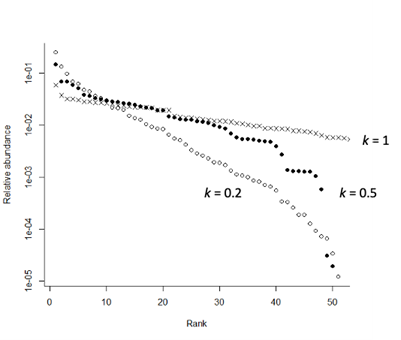
\includegraphics[keepaspectratio]{diversity/data-image/power-fraction-relative-abundance.png}}

}

\caption{\label{fig-power-fraction-relative-abundance}}

\end{figure}%

\section{Comparing models}\label{comparing-models}

All our models produce different distributions of species abundances
(Figure~\ref{fig-comparing-models}). Some have more in common than
others. For example, the log series yields a more even distribution of
individuals among species than the geometric series, but both tend to
have a low number of very abundant species and a large proportion of
rare species. In fact, the log species is predicted to occur as a result
of the same arrival model described by the geometric series, but here
the interval between the arrival of species into an unsaturated habitat
is random rather than regular. In the real world, it is most applicable
where only one or a few factors drive the community assemblage - for
example, on a forest floor, the main factor driving the community
assemblage might be the availability of light.

\begin{figure}

\centering{

\pandocbounded{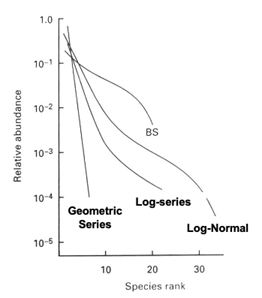
\includegraphics[keepaspectratio]{diversity/data-image/comparing-models.png}}

}

\caption{\label{fig-comparing-models}A comparison of rank abundance
curves generated by geometric series, log-series and log-normal models.
The geometric series is characterized by a straight line, species poor,
uneven community. The log series tends to be more species rich and more
even but retains a number of very common species that may dominate. The
log normal model is characterized by greater evenness, with some rare
species and few very common ones, and many intermediately-ranked species
with similar relative abundance.}

\end{figure}%

In contrast, log normal communities are diverse communities sampled with
a high level of effort. Compared to the geometric series and the log
series, log normal communities have a high species richness and a high
level of evenness: 99\% of species will occur within ±3 standard
deviation of the mean. This evenness occurs because many small factors
act on the abundance of each species, driving them all back towards the
mean (you may remember this as the central limit theorem from your
mathematics lessons at school). If there are lots of individuals within
a population, then those are likely to reduce due to competition. If
there are not many individuals, their numbers are likely to increase,
and thus the species is likely to become less rare.

Of course, ultimately we need to know if any of these models are useful
when trying to understand the patterns of rarity and evenness in our
communities of interest. It is important to remember that the
observation of a pattern that is predicted by a model doesn't
necessarily validate the mechanisms that the model assumes; just because
the pattern looks the same as the model, it doesn't necessarily mean
that the species arrived at the same end point in the same way as the
model implies.

In practice, usually more than one model will fit the real data quite
well. As researchers, we hope that one or two models will fit the data
particularly well: we are looking for statistical analyses to guide and
support our evaluation of biological meaningfulness, not to replace it.
We can then consider the underlying mechanisms in the sample location,
and choose the `best' model(s) that match both the patterns of rarity
and commonness that we see and the likely underlying mechanisms for that
environment and set of species.

\section{References}\label{references-3}

Bazzaz FA (1975). Plant species diversity in old-field successional
ecosystems in South Illinois. Ecology 56: 485-488.
https://doi.org/10.2307/1934981

Hill JK, Hamer KC, Lace LA, Banham WMT (1995). Effects of selective
logging on tropical forest butterflies on Buru, Indonesia. Journal of
Applied Ecology 32: 754-760.

\chapter{Patterns of species
richness}\label{sec-patterns-species-richness}

\section{TL;DR}\label{tldr}

The take home message from Chapter~\ref{sec-patterns-species-richness}
is that we don't have to eyeball species accumulation curves constructed
from observed species richness data to guess what true species richness
is. There are estimators to do this for you. These take into account the
number and relative abundance of species in the observed data, and may
be more or less affected by representation of rare species in the
dataset. Together with sampling locations at local and regional scales,
these can help better understand patterns of species richness across the
landscape.

\section{Observed versus true species
richness}\label{observed-versus-true-species-richness}

Species abundance models help us understand patterns of relative
abundance: how individuals are distributed among species. Species
richness estimates tell us how many species are present. In
\textbf{?@sec-species-richness-overview}, we established that species
accumulation curves change with commonness and rarity, and with sampling
effort. This is in part because as sampling effort increases, the curve
begins to encapsulate different processes and the scales that these
occur at. Patterns of species accumulation depend on a range of factors
such as the average species richness of a single sample and the
community at large, and the variability among samples, and among
communities.

Two communities can differ in many respects, which may affect how we
view their respective species richness, and the shape of the species
accumulation curve
(Figure~\ref{fig-representative-species-accumulation-curves}). In
practice, this means that it's important to consider how a sampling
protocol may affect the answer to the research question. For example,
expressing sampling effort as the number of quadrats used may present a
slightly different curve to expressing sampling effort as the number of
plant individuals sampled.

\begin{figure}

\centering{

\pandocbounded{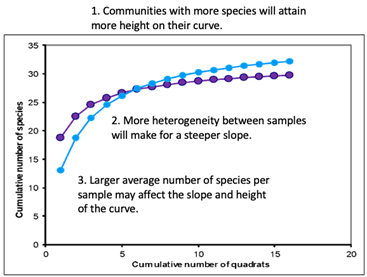
\includegraphics[keepaspectratio]{diversity/data-image/representative-species-accumulation-curves.png}}\{fig-alt
= ``Two representative species accumulation curve, with the number of
quadrats representing the sampling effort on the x axis, and the
cumulative number of species on the y axis.

Communities with more species will attain more height on the curve. More
heterogeneity between samples will make for a steeper slope. And a
larger average number of species per sample may affect the slope and
height of the curve.''\}

}

\caption{\label{fig-representative-species-accumulation-curves}Two
representative species accumulation curves, with the number of quadrats
representing the sampling effort on the x axis, and the cumulative
number of species on the y axis. Communities with more species will
ultimately attain more height on the curve. More heterogeneity between
samples will make for a steeper slope. A larger average number of
species per sample may affect the slope and height of the curve.
Sampling effort affects which one `looks' more species rich.}

\end{figure}%

One way to mitigate for this is to estimate `true' species richness from
our rank abundance data: what is the asymptotic value, or the point at
which the curve plateaus. There are a number of estimators for true
species richness: * \textbf{Parametric methods} fit a model to species
rank abundance data, and model the species accumulation curve from this
data. * \textbf{Non-parametric methods} use estimators known to converge
rapidly towards the asymptote, by applying different correction factors
depending on the rarity of species within the sample data.

The log series model that you encountered in
Chapter~\ref{sec-abundance-and-evenness} is an example of a parametric
method: the equation calculates the expected number of species with
\emph{n} individuals, which allows an estimate of how many species there
are in total.

Non-parametric methods use information about the species that have been
observed to infer how many species have not been observed. We are not
going to go into mathematical details about any of these now, but you
can read more about them in the workshop case studies. They follow the
same characteristic equation, where predicted species richness started
with the observed species richness, and is adjusted based on a function
of the relative abundance of species, often focusing on the number of
rare species (e.g.~those with only 1 or 2 individuals), and the number
of sites, because the more sampling you have done, the more likely it is
that you've seen everything.

The following three equations follow the same approximate formula:
Predicted species richness (\(S_p\)) is equal to the observed species
richness (\(S_0\)) plus a correction term.

\subsection{Jackknife}\label{jackknife}

\[
S_p = S_0 + a_1({{N - 1}\over N})
\] Where: \(a_1\) is the number of species that only occur once \emph{N}
is the number of sites in the dataset

\subsection{Chao}\label{chao}

\[
S_p = S_0 + {a_1~^2\over 2a_1}({{N - 1} \over N})
\] \#\#\# Bootstrap \[
S_p = S_0 + \sum^{S_0}_{i = 1} (1 - {Y_i \over N})^N
\] Where: \(Y_i\) is the number of individuals in species \emph{i}

\section{Case study Aquatic macrophytes and species
richness}\label{case-study-aquatic-macrophytes-and-species-richness}

Species richness estimators in action can be quite powerful. Bini et
al.~(2001) conducted a study of aquatic macrophytes in a South American
floodplain, sampling 20 lagoons in October and November of 1999 to
estimate the species richness of three regions. The researchers
intensively sampled these enclosed lagoons, and were fairly sure that
there were fifty species in total
(Figure~\ref{fig-bini-accumulation-curves}).

\begin{figure}

\centering{

\pandocbounded{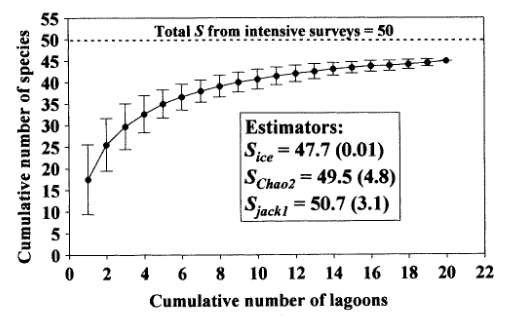
\includegraphics[keepaspectratio]{diversity/data-image/bini-accumulation-curves.png}}

}

\caption{\label{fig-bini-accumulation-curves}}

\end{figure}%

However, when the lagoons were considered individually, one area of
sampling appears to be much lower in species richness than the other two
(Figure~\ref{fig-bini-lagoons}). Indeed, when effort is measured by time
rather than sample, the Ivenheima region doesn't become any more species
rich with increased effort: it didn't matter how long the researchers
looked, they were never going to find more than ten species at this
particular site. In this instance, an increase in sampling effort
wouldn't have led to finding more species, as is assumed in the models
above.

\begin{figure}

\centering{

\pandocbounded{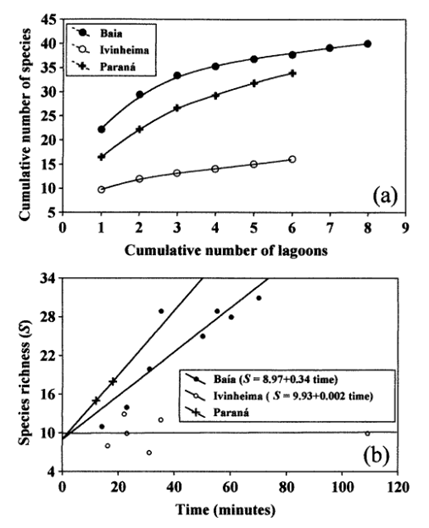
\includegraphics[keepaspectratio]{diversity/data-image/bini-lagoons-sampling.png}}

}

\caption{\label{fig-bini-lagoons}}

\end{figure}%

\section{Why do patterns of species richness
exist?}\label{why-do-patterns-of-species-richness-exist}

Why do some communities have more species than others? Are there
patterns or gradients of species richness? If so, why do these exist?
Broadly speaking, there are four factors that affect species richness: *
Geographical factors: latitude, altitude, depth (under water) * Factors
correlated with latitude: climate, energy, productivity, environment *
Factors not correlated with latitude: physical disturbance, isolation,
heterogeneity * Biotic factors: Predation/parasitism, competition,
succession

Geographic factors vary spatially, and slowly over time. Factors
correlated with latitude can vary both spatially and temporally due to
differences in e.g.~climate and weather. Factors may not be correlated
with latitude: for example, the physical levels of disturbance of a
site, or a site's isolation. Are you sampling an island a long way from
the mainland? Are resources evenly spread, or are they patchy and
heterogenous? Finally, biotic factors might also be influencing your
site, such as predation and parasitism; these vary with space, time and
the community that is present.

We may also need to consider how saturated a community is, by comparing
``local'' richness against ``regional'' richness. Here, a local area is
one in which the species within it can encounter and interact with each
other in ecological time, whereas a region is larger. Dispersal rates
within local sites within a region should be greater than the dispersal
rates between different regions, meaning that individuals should be
moving much more within the region than they are moving between regions.

An unsaturated population follows a straight line relationship, implying
that where local samples are more diverse, the regional richness is also
greater. With the saturated community, the local richness reaches a
plateau: it doesn't matter how much richer the regional richness gets,
the local richness cannot increase. This may occur in regions that are
limited in space, for example.

To illustrate this, we can look at the species richness of fish in
African rivers (Figure~\ref{fig-local-vs-regional-species-richness} a)
and ants in soil litter
(Figure~\ref{fig-local-vs-regional-species-richness} b) to see
unsaturated and saturated communities respectively. Hugueny and Paugy
(1995) sampled ten rivers (the regions) by looking for fish in a number
of small pools (the local areas). They calculated the local species
richness as the average number of species found in each pool in a river,
and calculated total river species richness using the whole set of
samples from that river. Where individual pool samples were more
diverse, the whole river was more diverse: this community had room for
more diversity at both the regional and local scales
(Figure~\ref{fig-local-vs-regional-species-richness} a). The river
species richness was well explained by the size of the catchment area:
the larger the catchment area, the more diverse the river.

In contrast, Soares et al.~(2001) sampled ten forest fragments (the
regions) by sampling from ten quadrats (the local areas) within each
fragment. Again, they calculated average local species richness from the
quadrats taken individually within each region, and regional species
richness by pooling the data from the ten quadrats. Although some
fragments had much higher species richness, individual quadrats had an
average of 18 or 20 ant species. The local species richness reached a
plateau, regardless of the regional species richness
(Figure~\ref{fig-local-vs-regional-species-richness} b). Factors such as
the space available, or social behaviour of the ants, are limiting local
species richness.

\begin{figure}

\centering{

\pandocbounded{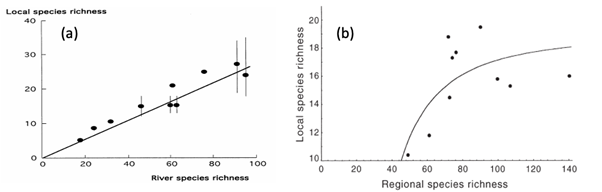
\includegraphics[keepaspectratio]{diversity/data-image/local-vs-regional-species-richness.png}}

}

\caption{\label{fig-local-vs-regional-species-richness}Local species
richness against regional species richness. (a) For fish in African
rivers, local species richness (pools) increase with river species
richness, implying that this is an unsaturated community (Hugueny and
Paugy 1995). (b) For ants in soil litter, quadrats (local sites) never
contain more than 18-20 species of ant, even when the wider forest
fragment (the region) has greater species richness (Soares et al.~2001).
This is a saturated community: it doesn't matter how species rich the
region becomes, there is a limit to how rich the local areas can
become.}

\end{figure}%

\section{References}\label{references-4}

Bini et al.~(2001) Species richness and ß-diversity of aquatic
macrophytes in the Upper Paraná River floodplain. Arch. Hydrobiol. 151:
511-525

Hugueny B, Paugy D (2001). Unsaturated fish communities in African
rivers. The American Naturalist 146(1): 162-169.

Soares SM, Schoereder JH, DeSouza O. (2001), Processes involved in
species saturation of ground-dwelling ant communities (Hymenoptera,
Formicidae). Austral Ecology, 26: 187-192.
https://doi.org/10.1046/j.1442-9993.2001.01101.x

\chapter{Ecological diversity}\label{sec-ecological-diversity}

\section{TL;DR}\label{tldr-1}

Diversity indices combine how many species there are (richness) and
species abundance (evenness) into a single metric, to more easily
compare large data sets across different temporal and spatial scales.
There are many different ways to calculate diversity indices, and each
one has its own underlying models, assumptions and nuances for
interpretation. Boiling your analysis down to a single metric is usually
not a good idea; consider using multiple diversity indices with
different assumptions, and explore the data at different scales, with an
exploration of variation (error/uncertainty/sampling bias) in your
analysis, to ensure a more robust set of conclusions.

\section{Species diversity: species richness and rank
abundance}\label{species-diversity-species-richness-and-rank-abundance}

Rank abundance plots and species richness estimators tell us quite a lot
about ecological diversity within a community, but as tools to compare
many communities, in the context of underlying factors driving those
patterns, they are relatively complex. Species rank abundance
distributions give us a measure of the community structure and the
relative abundance. Models can tell us what processes might be
generating that structure, and start to explain some of the dynamics and
processes driving those distributions. Species richness tells us how
many species are present in a community, but we may need to account for
the differences in observed vs true species richness depending on our
sampling effort. Diversity indices try to pull these concepts together
into a single representative value: quantitative measures that reflect
\textbf{how many species} there are (richness) and simultaneously take
into account \textbf{how evenly the individuals are distributed} among
the species (evenness). There are lots of tools available for us to do
this. These can be:

\begin{itemize}
\tightlist
\item
  Parametric, which make assumptions about the underlying processes or
  distribution of the data. You will be familiar with many of these from
  your statistics knowledge:

  \begin{itemize}
  \tightlist
  \item
    Samples should be independent;
  \item
    Data should be normally distributed;
  \item
    Samples should have been taken at random.
  \end{itemize}
\item
  Non-parametric, which make far fewer assumptions about the
  distribution of the data.
\end{itemize}

\subsection{Log series alpha}\label{log-series-alpha}

One of the most common of the parametric diversity indices is the log
series alpha. Recall that the log series
(Chapter~\ref{sec-abundance-and-evenness}) is a series of calculations
that estimates the number of species in our community that are
represented by one individual, two individuals, three
individuals\ldots{} all the way up to \emph{n} individuals. Alpha is
approximately the number of species with 1 individual, i.e.~the number
of rare species. In the example of butterflies on Buru, Indonesia (Hill
et al.~1995), the alpha value for the unlogged site was 7.94, slightly
higher than for the logged site, which was 6.99. There were also more
individuals for the same effort of sampling in the unlogged site than in
the logged site, and there are more total species in the unlogged than
the logged. Based on these calculations, logging has clearly had an
effect on the community, leading to fewer individuals and fewer species
present.

\subsection{Case study: Barro Colorado
Island}\label{case-study-barro-colorado-island}

Another real world dataset example comes from Barro Colorado Island.
Barro Colorado island is an artificial island that was created when a
dam was built to create the Panama canal
(Figure~\ref{fig-barro-colorado-island}). The raised water levels cut
off a previously connected area of land into an island, which was
declared a nature reserve. The Smithsonian institute have been
performing surveys on it since its creation in the 1980s, so we have
some continuous data about the environment and communities in that
region.

Early in the surveying, a number of 50 hectare plots were established,
and every tree above a certain stem diameter in each of those plots was
recorded. Plot 53, for example, has 600 individuals representing
approximately 83 individuals, while plot 23 has about 340 individual
trees and nearly 100 species (Figure~\ref{fig-barro-colorado-island}).
Many plots have more than 100 species of tree - much higher than
temperate woodland!

\begin{figure}

\centering{

\pandocbounded{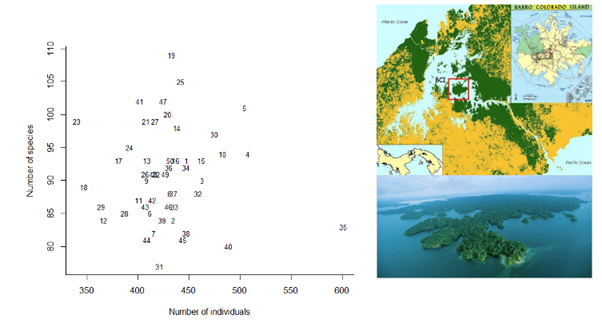
\includegraphics[keepaspectratio]{diversity/data-image/barro-colorado-island.pdf}}

}

\caption{\label{fig-barro-colorado-island}There is no clear relationship
between the number of individual trees in a Barro Colorado Island (BCI)
plot (tree density; x axis) and the number of species found there. BCI
is located in Panama, west of the Panama Canal.}

\end{figure}%

But which of these plots is the most diverse? We can't just assume it's
plot 19 with the most species (Figure~\ref{fig-barro-colorado-island}),
because the tree densities also vary. How do these plots compare if we
use the log series alpha to measure diversity through the lens of rare
species abundance? There is a strong, positive relationship between the
number of species and the log alpha estimate of a site
(Figure~\ref{fig-bci-log-alpha}). This suggests that sites with greater
species richness also have more rare species. However, there is a lot of
variation: sites with the same observed species richness may still
differ in our log series alpha estimate of diversity.

\begin{figure}

\centering{

\pandocbounded{\includegraphics[keepaspectratio]{diversity/data-image/bci-log-series.pdf}}

\part{Practicals}

This chapter contains the materials associated with the various
practicals carried out in the Practical Ecology module. You may find
this useful to refer back to when you're planning your sampling for the
Field Course portion of the module.

Chapter~\ref{sec-plantago-practical} Chapter~\ref{sec-pitfall-practical}

\chapter{\texorpdfstring{\emph{Plantago} distributions
practical}{Plantago distributions practical}}\label{sec-plantago-practical}

\href{files/BIO00036I\%20Plantago\%20Practical.docx}{Download the
practical files}

\section{Practical overview}\label{practical-overview}

In this practical, you will be investigating the spatial structure of a
population of the ribwort plantain (\emph{Plantago lanceolata}) on a
grass bank near the Department of Biology.

In this practical, you will:

\begin{itemize}
\tightlist
\item
  Use quadrats of two different sizes to count individual plants on the
  grass bank.
\item
  Submit your data to the class spreadsheet.
\end{itemize}

\section{Background to distributions}\label{background-to-distributions}

The spatial structure of a population can be characterised by whether it
is random, aggregated, or regular (Figure~\ref{fig-dispersal}).

\begin{enumerate}
\def\labelenumi{\arabic{enumi}.}
\item
  Random: the position of each individual is independent of the position
  of every other individual. You could think of this as the absence of
  any pattern. It might come about through the random scattering of
  seeds on the ground surface.
\item
  Aggregated (underdispersed): individuals tend to occur in clumps close
  together. Such a pattern can arise if there is localised dispersal
  (e.g.~seeds stay very close to their parent), or if there are only
  certain microsites in which individuals can live.
\item
  Regular (overdispersed): individuals tend to occur in a rather evenly
  spaced manner. This can happen if there is strong competition between
  neighbouring individuals leading to death of some of them.
\end{enumerate}

\centering{

\pandocbounded{\includegraphics[keepaspectratio]{practicals/data-image/dispersal.png}}

}

\subcaption{\label{fig-dispersal}Three examples of spatial patterns of
individuals: from left to right, these are overdispersed or regular,
random, and aggregated or clustered.}

The spatial structure is important because it may give clues as to the
dynamic processes which have taken place in the past giving rise to the
present distribution in space. It also sets the path for dynamics in the
future in circumstances where individuals interact primarily with their
immediate neighbours.

\section{Learning Outcomes}\label{learning-outcomes}

By the end of this practical, you should be able to:

\begin{itemize}
\tightlist
\item
  Design an experiment to decide whether the spatial pattern of plantain
  individuals is random, regular, or aggregated
\item
  Be familiar with the use of quadrats to standardise sampled areas.
\item
  Collect the data to test your hypothesis.
\item
  Be prepared to use statistical distributions to analyse and interpret
  your data.
\end{itemize}

\section{Instructions}\label{instructions}

\begin{itemize}
\tightlist
\item
  A briefing presentation will be given at the beginning of the
  practical, with details of what you will need to do explained. In the
  practical, you will meet in the Biology teaching lab to be briefed and
  collect equipment. You will carry out the sampling on campus and then
  return your equipment and submit your data.
\item
  After the briefing we will move to the grass outside Biology to carry
  out the sampling.
\item
  Wear sensible footwear, warm clothes and, if necessary, waterproofs.
\item
  You will be working in small groups to collect data on the location of
  quadrats and the number of plantains within the quadrat.
\end{itemize}

\subsection{Practical techniques you should be familiar with before this
practical}\label{practical-techniques-you-should-be-familiar-with-before-this-practical}

\begin{itemize}
\tightlist
\item
  Keeping a laboratory notebook
\end{itemize}

(If you are unfamiliar with these techniques or need a refresher before
the practical, please visit the practical skills section on the
\href{https://xerte.york.ac.uk/play.php?template_id=4175\#page1}{VLE
Skills Hub})

\section{New practical techniques learnt in this
practical}\label{new-practical-techniques-learnt-in-this-practical}

\begin{itemize}
\tightlist
\item
  This practical allows you to practise sampling fixed areas using
  quadrats and consolidate sampling techniques you will also have a
  chance to test using LEGO.
\end{itemize}

\section{Skills that can be signed off during this
practical}\label{skills-that-can-be-signed-off-during-this-practical}

\begin{itemize}
\tightlist
\item
  Keeping a laboratory notebook
\end{itemize}

\section{Safety}\label{safety}

\begin{itemize}
\tightlist
\item
  This practical will partly be held outside at a field site on campus.
  You should remain with the group and in contact with the academic
  staff and/or demonstrator at all times
\item
  Wear sensible footwear, warm clothes, and, if necessary, waterproofs.
  Be careful when carrying equipment to the field site
\item
  No smoking or vaping
\item
  The module organiser has a first aid kit (e.g.~for cuts).
\end{itemize}

\section{Experimental protocol}\label{experimental-protocol}

\subsection{Overview of practical}\label{overview-of-practical}

The basic idea is to count the number of plantain plants in randomly
positioned quadrats, and to look at the variation present when the data
from a large number of quadrats are put together. Imagine placing
quadrats onto the different spatial distributions described and
illustrated above, the size of the quadrat being either small or large

If the pattern is regular, all the quadrats will contain more or less
the same number of plants. At the other extreme, if the plants are
aggregated, some of the quadrats will contain many plants and others
will contain none. If the pattern is random, the frequency distribution
of number of plants per quadrat will have a Poisson distribution. What
would the data look like if the quadrat is approximately the same size
as a plant?

Work in small groups.

Make sure you're confident in your identification of \emph{Plantago
lanceolata.} Individuals may be quite small and could potentially be
confused with other species such as the common daisy \emph{Bellis
perennis}.

Each group should work with quadrats of two sizes: 40 x 40 cm (small)
and 1 x 1 m (large). Each of these can be generated using the large,
subdivided quadrats.

An `origin' and x and y `axes' for the grass bank will be marked out
with stakes and tape measures so that you are all working in the same
space.

Use random number tables or a random number generator on your phone, so
that you can choose a random x and y coordinate on which to place the
quadrat. Using the small quadrat first, count the number of individual
plants present. Repeat this using the larger quadrat, keeping the two
data sets separate. Aim to get counts for both quadrat sizes for around
15 coordinates. We need to have a large number of quadrats of each size
to be able to look at the frequency distribution, and we will end up by
pooling all the data collected for each quadrat size.

Record all your data using the table on the next page, and when you have
finished, enter it into the Google sheet that is on the VLE.

\subsection{Before you leave}\label{before-you-leave}

\begin{itemize}
\tightlist
\item
  Tell a member of staff that your group has finished sampling
\item
  Return all equipment to the location that you got it from
\end{itemize}

\chapter{Sampling Ground-Dwelling Insects and Small
Animals}\label{sec-pitfall-practical}

\href{files/BIO00036I\%20Animal\%20Sampling\%20Practical.docx}{Download
the practical files}

\section{Overview}\label{overview}

Communities of plants and animals are notoriously difficult to study.
Each species in the community will tend to occur at a different density
(e.g.~number of individuals per \(m^2\)) in the environment and may
follow different patterns of spatial distribution too (aggregated,
random or regular). Ecologists have approached this complex set of
information through a variety of means, trying to see the wood despite
the trees (i.e.~appreciate how the whole community was organised without
being mesmerised by too much detail).

In this practical, you are going to be introduced to a simple technique
to sample ground dwelling arthropods, and to identify vertebrate
presence.

In these practicals, you will:

\begin{itemize}
\tightlist
\item
  Set up pitfall traps to sample ground dwelling arthropods
\item
  Set out animal tracking tunnels as a way of detecting small animal
  activity
\end{itemize}

\section{Learning outcomes}\label{learning-outcomes-1}

By the end of these practicals, you should be able to:

\begin{itemize}
\tightlist
\item
  Set up pitfall traps and conduct a field experiment to determine
  whether ground arthropods might be attracted or deterred by different
  fluids used traditionally in pitfall traps.
\item
  Set up animal tracking tunnels and identify what small mammals, birds
  and invertebrates are present in the study area.
\end{itemize}

\section{Assessment}\label{assessment}

This practical is not directly assessed, but techniques may be used
during the field course, and the data may be used for practising
analyses.

\section{Coordinating instructions}\label{coordinating-instructions}

\begin{itemize}
\tightlist
\item
  A briefing presentation will be given by video and written
  instructions on the VLE, with details of what you will need to do
  explained. In practical 1, you will collect equipment from the
  department and set out the pitfall traps and tracking tunnels. In
  practical 2, you will collect in the equipment, then return to the
  department lab to do identification.
\item
  Your timetable for weeks 7 \& 8 will show when you need to attend
  sessions.
\item
  The practicals will take place in the Biology teaching labs and
  locally on campus
\item
  Wear sensible footwear and, if necessary, waterproofs.
\item
  \textbf{You should work in your bird-based module groups.}
\end{itemize}

\section{Practical techniques you should be familiar with before this
practical}\label{practical-techniques-you-should-be-familiar-with-before-this-practical-1}

\begin{itemize}
\tightlist
\item
  Keeping a laboratory notebook.
\end{itemize}

If you are unfarmiliar with these techniques or need a referesher before
the practical please visit the practical skills section of the skills
hub on the VLE.

\section{New practical techniques learnt in this
practical}\label{new-practical-techniques-learnt-in-this-practical-1}

\begin{itemize}
\tightlist
\item
  This practical allows you to learn pitfall trapping, tracking tunnel
  use, and ID of invertebrates and footprints
\end{itemize}

\section{Skills that can be signed off during this
practical}\label{skills-that-can-be-signed-off-during-this-practical-1}

\begin{itemize}
\tightlist
\item
  Keeping a laboratory notebook
\end{itemize}

\section{Safety}\label{safety-1}

\begin{itemize}
\tightlist
\item
  This practical will partly be held outside at a field site on campus.
  You should remain with the group and in contact with the module
  organiser and/or demonstrator at all times. Wear sensible footwear
  and, if necessary, waterproofs. Be careful when carrying equipment to
  the field site. No smoking.
\item
  Soil corers are very sharp and you must be extremely careful when you
  carry them and use them. Always point the cutting edge away from you.
  Wear gardening or other thick gloves when handling them.
\item
  The antifreeze and detergent solutions are irritants if you get them
  on your skin or in your eyes, so take care with them. Wear disposable
  gloves and eye protection when you are pouring the solutions. Should
  the antifreeze or detergent solutions come in contact with your skin
  or eyes rinse immediately with water and notify the module organiser
  or demonstrator.
\item
  Should they be needed in the field, the module organiser has a first
  aid kit (e.g.~for cuts) and container of water (e.g.~to rinse skin or
  eyes that have come in contact with chemicals).
\item
  You may wish to wear disposable gloves when applying paint and bait to
  the tracking tunnels. Wash your hands after handling the animal
  tracking tunnels.
\end{itemize}

\section{Experimental protcol}\label{experimental-protcol}

\subsection{Practical 1}\label{practical-1}

\subsubsection{Overview of practical}\label{overview-of-practical-1}

In the first practical, you are going to be introduced to and set up, a
very simple yet efficient technique to sample ground dwelling
arthropods, called pitfall traps. This technique relies on the natural
activity (dwelling and crawling) of ground arthropods to work. The more
active an individual is, the more likely it is to fall and be trapped in
the pitfall. This adds a complicating factor, however, as the abundance
of the species in the samples will not just reflect their abundance in
the environment but their relative level of activity as well (which may
vary between taxa, between sexes, or with the size of the individual).
In the case of pitfalls, one also has to consider carefully the type of
fluid used as preservative at the bottom of the traps. Some may emit a
smell which may attract or alternatively repel some species more than
others, further distorting our measure of their relative abundance.

In the second part of the practical you will have the chance to set up
animal tracking tunnels to give you experience detecting small animals.

\subsubsection{Sampling ground dwelling
insects}\label{sampling-ground-dwelling-insects}

A pitfall trap is a very simple device for catching ground dwelling
arthropods. Essentially it is a cup that is dug into the soil with the
rim slightly below the soil level. Passing insects simply walk into the
trap, and like the spider in your bath, are unable to climb out
(especially if the trap contains some preservative fluid).

There are all sorts of pros and cons associated with pitfall trapping.
One factor that could affect what and how much is caught is the solution
placed in the traps to kill and preserve the catch. This experiment
examines the effects of different solutions on what is caught. It also
allows you to compare and contrast the organisms found using this
method. The pitfall traps will be located near the Biology department,
along a habitat gradient that includes different tree species and ground
cover. We will examine the catches next week in Practical 2.

\begin{enumerate}
\def\labelenumi{\arabic{enumi}.}
\tightlist
\item
  To determine whether there is a difference between treatments we will
  adopt a randomised block design. This means that each group will set
  up a `block' of 4 traps each, with the 4 treatments randomised within
  each block (Figure~\ref{fig-randomised-block}).
\end{enumerate}

\centering{

\pandocbounded{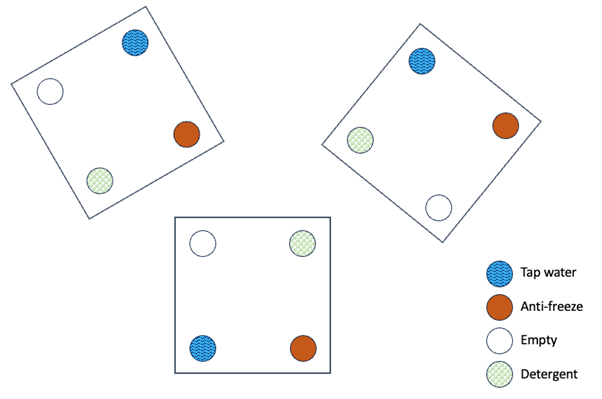
\includegraphics[keepaspectratio]{practicals/data-image/randomised-block-design.png}}

}

\subcaption{\label{fig-randomised-block}}

\begin{enumerate}
\def\labelenumi{\arabic{enumi}.}
\setcounter{enumi}{1}
\item
  Within each block you will need four traps (plastic cups quarter-full
  with fluid) with one of the following, either: tap water, 25\%
  anti-freeze, 10\% detergent (washing-up liquid) or empty. \textbf{Wear
  goggles and gloves when handling the anti-freeze and detergent}.
\item
  Each group will set up one or two metre-square blocks of 4 traps (see
  Figure~\ref{fig-randomised-block}). If there are four or more people
  in the group, aim to do two blocks. If there are three or fewer, you
  can do one block and then decide if you want to do a second. There
  should be 8-16 blocks completed by the class as a whole. Note that the
  trap spacing within the blocks is regular, and the blocks will be
  evenly spaced along the grass bank near Biology; it is the allocation
  of the different treatments within each block that is randomised.
\item
  All four traps within each block should be placed within one habitat
  (e.g.~grass, or bare earth), rather than straddling two or more
  habitats.
\item
  To set the cups in the ground use the soil corer to remove sufficient
  soil to allow the cup to sit snugly in the ground with the lip just
  below the surface of the soil. Wear gloves when handling the soil
  corer, when digging it in and when removing soil from it. Once
  securely placed, half fill the appropriate cups with the different
  preservative solutions. The removed soil cores should be stacked at
  the edge of the field site, so that they can be replaced when the
  pitfall traps are removed in Practical 2.
\end{enumerate}

\subsubsection{Setting tracking tunnels}\label{setting-tracking-tunnels}

A tracking tunnel is a very simple device for collecting presence data
on small mammals, birds and invertebrates. It comprises of two parts,
the tunnel and the tracking plate that slides into the bottom of the
tunnel. Bait is placed in the centre of the trap, and strips of tape are
painted so that animals crossing the tape create footprints on the
tracking paper when they leave. As a class, we will set out three
tunnels. We will examine the tracking paper next week, and identify any
footprints that have been captured.

\begin{enumerate}
\def\labelenumi{\arabic{enumi}.}
\tightlist
\item
  The tunnel is made of corrugated plastic, and should be folded up to
  make a triangular tunnel (there are Velcro pads and plastic grips to
  keep it in place). See Figure~\ref{fig-assembled-tracking-tunnel}.
\end{enumerate}

\centering{

\pandocbounded{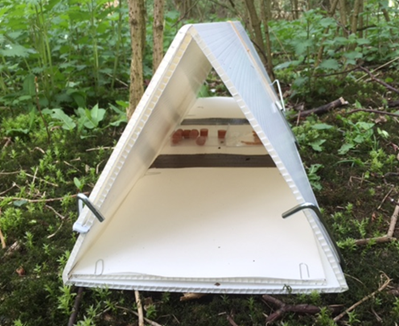
\includegraphics[keepaspectratio]{practicals/data-image/assembled-tracking-tunnel.png}}

}

\subcaption{\label{fig-assembled-tracking-tunnel}The assembled tracking
tunnel, with bait and paint.}

\begin{enumerate}
\def\labelenumi{\arabic{enumi}.}
\setcounter{enumi}{1}
\tightlist
\item
  Fix 2 A4 sheets of paper to the tracking plate using paper clips
  inserted into the flutes of the plastic. Label the paper with the date
  and some identifying marks (e.g.~a group name). See
  Figure~\ref{fig-tracking-plate-setup}.
\end{enumerate}

\centering{

\pandocbounded{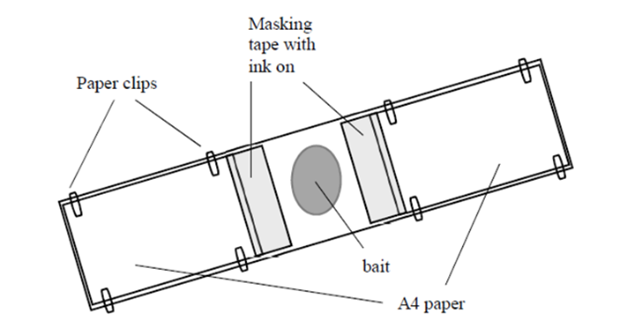
\includegraphics[keepaspectratio]{practicals/data-image/tracking-plate-setup.png}}

}

\subcaption{\label{fig-tracking-plate-setup}}

\begin{enumerate}
\def\labelenumi{\arabic{enumi}.}
\setcounter{enumi}{2}
\item
  Two square dishes are available to place in the middle of the tracking
  plate; you may wish to secure these with masking tape.
\item
  Place two or three strips of masking tape either side of the bait
  dishes, so that any animal entering the tunnel will have to walk on
  them to reach the bait (width should be 8-10 cm). Paint these with
  tracking paint; this should be a mixture of 1 unit (e.g.~tbsp)
  non-toxic powder paint to 2 units vegetable oil.
\item
  Choose some bait from the available bait types, and add it to the bait
  dishes. You may wish to make a note of what bait types your group has
  chosen to use.
\item
  Once you have chosen a location for your tunnel, slide your tracking
  plate into the tunnel and secure the whole assembly to the ground
  using 6-8 tent pegs.
\end{enumerate}

You may find it useful to angle the pegs to keep the tunnel near the
ground, and/or use the hooked ends of the pegs to hold the ends of the
tunnel/tracking plate down.

\subsubsection{Before you leave}\label{before-you-leave-1}

\begin{itemize}
\tightlist
\item
  Tell a member of staff that your group has finished setting out your
  pitfall traps.
\item
  Take part in setting out a tracking tunnel.
\item
  Return all equipment to the location that you got it from.
\end{itemize}

\subsection{Practical 2}\label{practical-2}

\subsubsection{Overview of practical}\label{overview-of-practical-2}

In the practical today you will collect the pitfall traps and tracking
tunnels from the field before analysing them to identify the
invertebrates caught in the pitfall traps, and the animals that have
left footprints in your tunnels. These data will be uploaded to a google
spreadsheet. The pitfall trap data will be analysed later in the course
to determine the effect of the type of fluid used in the pitfall traps
on catch size by family. Both techniques may be used in field course
projects in the spring.

\subsubsection{Pitfall traps}\label{pitfall-traps}

The pitfalls with their contents need to be collected from the field and
their contents analysed. As you will remember, we organised the pitfalls
into a randomised block design.

\begin{enumerate}
\def\labelenumi{\arabic{enumi}.}
\tightlist
\item
  Collect each cup, cap it with one of the plastic lids provided, label
  it and tape the lid on securely. Carry them back to the lab in the
  buckets provided.
\end{enumerate}

The 4 pitfalls in block 1, need to be kept separate from those in block
2, etc. so a sensible labelling scheme is important if you have
collected more than one block. You also need to know what the treatment
was for each of your pitfall traps.

\begin{enumerate}
\def\labelenumi{\arabic{enumi}.}
\setcounter{enumi}{1}
\item
  Count the total number of invertebrates in each trap of each block and
  record them in your lab book according to the layout in table 1 in the
  appendix of the downloadable practical file.
\item
  For each of your 4 pots, sort their contents into the following
  categories, ants, beetles, woodlice, myriapods (centipedes and
  millipedes), spiders, earthworms, molluscs (slugs and snails). Add
  columns for additional families if required.
\item
  Enter your counts into your lab book and transcribe this data into the
  Google spreadsheet linked on the VLE so that class data can be
  collated. Each group should enter their data onto the correct row for
  their pitfall trap data; these will have been set up for you in
  advance.
\end{enumerate}

\subsubsection{Tracking tunnels}\label{tracking-tunnels-1}

The tracking tunnels should have footprints in them of the creatures
that have been through the traps to take the bait.

\begin{enumerate}
\def\labelenumi{\arabic{enumi}.}
\item
  Use the ID cards provided to identify what small creatures have been
  traipsing through your tracking tunnel. Record this information in
  your lab book.
\item
  Enter your data into the Google spreadsheet linked on the VLE so that
  class data can be collated.
\end{enumerate}

\subsubsection{Before you leave}\label{before-you-leave-2}

\begin{itemize}
\tightlist
\item
  Make sure your data has been recorded on the Google sheet.
\item
  Tidy your workstation and put away any unused equipment.
\item
  Place used liquids into the relevant labelled containers.
\item
  Place dead invertebrates into waste bags.
\item
  Place live invertebrates into the bag labelled `Live invertebrates'.
\item
  Place used Petri dishes into the tray labelled `Used Petri dishes'
\item
  Rinse used plastic cups and lids and place in the tray labelled `Used
  cups and lids'
\item
  Leave used tracking tunnel papers on the bench. Make sure they include
  your group name and date, and have any identifications clearly
  labelled on the sheets.
\item
  Remove your lab coat and wash your hands before leaving the lab.
\end{itemize}

}

\caption{\label{fig-bci-log-alpha}}

\end{figure}%




\end{document}
